\documentclass[12pt,a4paper]{report}

% ==========================================
% CÁC GÓI THƯ VIỆN CHUẨN TIẾNG VIỆT (XELATEX / TECTONIC / BREWLITE STYLE)
% ==========================================
\usepackage{fontspec}
\setmainfont{Times New Roman}
\usepackage{geometry}
\geometry{
    a4paper,
    left=2.5cm,
    right=2.0cm,
    top=2.4cm,
    bottom=2.4cm
}

\renewcommand{\contentsname}{Mục lục}
\renewcommand{\listfigurename}{Danh mục hình ảnh}
\renewcommand{\listtablename}{Danh mục bảng biểu}
\renewcommand{\chaptername}{Chương}
\renewcommand{\figurename}{Hình}
\renewcommand{\tablename}{Bảng}
\renewcommand{\bibname}{Tài liệu tham khảo}

\usepackage{amsmath,amssymb,amsfonts}
\usepackage{graphicx}
\usepackage{booktabs}
\usepackage{longtable}
\usepackage{array}
\usepackage{multirow}
\usepackage{float}
\usepackage{caption}
\usepackage{subcaption}
\usepackage{enumitem}
\usepackage{xcolor}
\usepackage{titlesec}
\usepackage{fancyhdr}
\usepackage{tikz}
\usetikzlibrary{positioning,shapes.geometric,arrows.meta,calc}
\usepackage{hyperref}

% Đường dẫn tìm hình ảnh (logo ở cùng thư mục, biểu đồ ở figures/)
\graphicspath{{./}{figures/}}

% Bảng màu đồng bộ với mẫu bìa BrewLite Assignment 2
\definecolor{CoverBlue}{HTML}{263CBF}
\definecolor{primaryblue}{RGB}{18, 58, 114}
\definecolor{darkgray}{RGB}{60, 60, 60}
\definecolor{softgray}{RGB}{245, 247, 250}
\definecolor{accentteal}{RGB}{13, 115, 119}

\hypersetup{
    colorlinks=true,
    linkcolor=primaryblue,
    citecolor=primaryblue,
    urlcolor=primaryblue,
    pdftitle={FPT Forecast Studio - Bao cao Do an Mon hoc Hoc may},
    pdfauthor={Truong Trong Phuc, Pham Khanh Nguyen, Che Van Nam, Do Dat}
}

% Định dạng tiêu đề Chương / Mục gọn đẹp, chuẩn báo cáo đại học
\titleformat{\chapter}[display]
  {\normalfont\huge\bfseries\color{primaryblue}}
  {\chaptertitlename\ \thechapter}{8pt}{\Huge}
\titlespacing*{\chapter}{0pt}{-10pt}{18pt}

\titleformat{\section}
  {\normalfont\Large\bfseries\color{primaryblue}}
  {\thesection}{0.8em}{}

\titleformat{\subsection}
  {\normalfont\large\bfseries\color{darkgray}}
  {\thesubsection}{0.8em}{}

% Header & Footer
\pagestyle{fancy}
\fancyhf{}
\fancyhead[L]{\small\textit{Báo cáo Đồ án Môn học: Học máy (Machine Learning)}}
\fancyhead[R]{\small\textit{FPT Forecast Studio}}
\fancyfoot[C]{\thepage}
\renewcommand{\headrulewidth}{0.4pt}

\setlength{\parindent}{0pt}
\setlength{\parskip}{0.48em}
\setlength{\emergencystretch}{3em}
\sloppy
\renewcommand{\baselinestretch}{1.24}
\setlist[itemize]{nosep,leftmargin=1.8em}
\setlist[enumerate]{nosep,leftmargin=1.8em}
\Urlmuskip=0mu plus 1mu\relax
\expandafter\def\expandafter\UrlBreaks\expandafter{\UrlBreaks\do\_\do\-}

\begin{document}

% ==========================================
% TRANG BÌA (THEO ĐÚNG MẪU BREWLITE-ASSIGNMENT2)
% ==========================================
\hypersetup{pageanchor=false}
\begin{titlepage}
  \thispagestyle{empty}
  \begin{center}
    {\normalsize TRƯỜNG ĐẠI HỌC SÀI GÒN}\\[3pt]
    {\normalsize KHOA CÔNG NGHỆ THÔNG TIN}\\[16mm]
    
\includegraphics[width=32mm]{logoITSGU.png}
  \end{center}

  \vspace{11mm}
  \begin{center}
    \color{CoverBlue}
    {\Large\bfseries HỌC MÁY (MACHINE LEARNING)}\\[3mm]
    \rule{\textwidth}{0.5pt}\\[4mm]
    {\large\bfseries Báo cáo Đồ án Môn học}\\[5mm]
    {\LARGE\bfseries FPT Forecast Studio}\\[3mm]
    {\Large Phân tích và dự báo lợi suất, giá đóng cửa cổ phiếu FPT bằng học máy}\\[4mm]
    \rule{\textwidth}{0.5pt}\\[4mm]
    {\normalsize Kiểm toán dữ liệu, kiểm soát rò rỉ, thực nghiệm đa mô hình và triển khai hệ thống}
  \end{center}

  \vfill
  {\color{CoverBlue}\small
    \hfill\begin{tabular}{@{}lll@{}}
      \textbf{GVHD:} & \multicolumn{2}{l}{Nguyễn Thanh Phước}\\[3mm]
      \textbf{SV:} & Trương Trọng Phúc & MSSV: 3124410287\\[1.5mm]
      & Phạm Khánh Nguyên & MSSV: 3124410239\\[1.5mm]
      & Chế Văn Nam & MSSV: 3124410217\\[1.5mm]
      & Đỗ Đạt & MSSV: 3124410054
    \end{tabular}
  }

  \vspace{11mm}
  \begin{center}
    {\small TP. HỒ CHÍ MINH, THÁNG 11/2026}
  \end{center}
\end{titlepage}
\hypersetup{pageanchor=true}

% ==========================================
% MỤC LỤC, DANH MỤC HÌNH ẢNH, DANH MỤC BẢNG BIỂU
% ==========================================
\pagenumbering{roman}
\tableofcontents
\clearpage
\listoffigures
\clearpage
\listoftables
\clearpage

% ==========================================
% BẢNG PHÂN CÔNG VÀ TỶ LỆ ĐÓNG GÓP TRUNG THỰC
% ==========================================
\chapter*{Bảng phân công nhiệm vụ và tỷ lệ đóng góp}
\addcontentsline{toc}{chapter}{Bảng phân công nhiệm vụ và tỷ lệ đóng góp}
\vspace{-6pt}

\begin{center}
\small
\renewcommand{\arraystretch}{1.16}
\setlength{\tabcolsep}{4pt}%
\resizebox{\ifdim\width>\textwidth\textwidth\else\width\fi}{!}{%
\begin{tabular}{@{}l>{\raggedright\arraybackslash}p{3.1cm}l>{\raggedright\arraybackslash}p{8.2cm}r@{}}
\toprule
\textbf{STT} & \textbf{Thành viên} & \textbf{MSSV} & \textbf{Nhiệm vụ} & \textbf{Tỷ lệ} \\
\midrule
1 & \textbf{Trương Trọng Phúc} & 3124410287 & \textbf{Setup \& Điều phối Train + Đợt 1 \& Đợt 8:} Thiết lập môi trường, chuẩn hóa pipeline chống rò rỉ và điều phối huấn luyện; thực hiện \textbf{Đợt 1} (Pipeline v2 CPU/Colab GPU) và \textbf{Đợt 8} (Walk-Forward 3y/5y/2018); cài đặt dự báo đệ quy, Block Bootstrap và viết Chương 1 \& 5. & 25\% \\[5pt]
2 & \textbf{Đỗ Đạt} & 3124410054 & \textbf{Phát triển REST API + Đợt 2 \& Đợt 6:} Xây dựng máy chủ \texttt{FastAPI} (\texttt{/health}, \texttt{/predict}, \texttt{/forecast}, \texttt{/backtest}), kiểm tra schema \texttt{Pydantic} và kiểm thử API; thực hiện \textbf{Đợt 2} (Robustness 63 cấu hình) và \textbf{Đợt 6} (Phân loại chọn lọc); viết Chương 3. & 25\% \\[5pt]
3 & \textbf{Phạm Khánh Nguyên} & 3124410239 & \textbf{Giao diện Studio + Đợt 3 \& Đợt 7:} Xây dựng giao diện \texttt{Streamlit FPT Forecast Studio} (4 không gian phân tích và 3 sơ đồ giải thích); thực hiện \textbf{Đợt 3} (Đối chiếu 3 nguồn Yahoo/Vietcap/KBS -- 112 điều kiện) và \textbf{Đợt 7} (Tách nến Gap/Body A/B); viết đầu Chương 4. & 25\% \\[5pt]
4 & \textbf{Chế Văn Nam} & 3124410217 & \textbf{Tiền xử lý \& Feature Engineering + Đợt 4 \& Đợt 5:} Làm sạch dữ liệu, cách ly nến lỗi và trích xuất đặc trưng nhân quả (16 chỉ báo $\to$ 6 return \texttt{Ridge6}); thực hiện \textbf{Đợt 4} (Cửa sổ \& lưới $\alpha$ Ridge) và \textbf{Đợt 5} (Recency Refit \& \texttt{bias60}); viết Chương 2 \& phần chọn mô hình Chương 4. & 25\% \\
\midrule
\multicolumn{4}{r}{\textbf{Tổng cộng}} & \textbf{100\%} \\
\bottomrule
\end{tabular}%
}
\end{center}

\clearpage
\pagenumbering{arabic}

% ==========================================
% CHƯƠNG 1: MÔ TẢ BÀI TOÁN VÀ TỔNG QUAN HỆ THỐNG
% ==========================================
\chapter{Mô tả bài toán và tổng quan hệ thống}

\section{Bối cảnh và động lực nghiên cứu}
Dự báo diễn biến thị trường chứng khoán là một trong những bài toán kinh điển nhưng đầy thách thức của Học máy (Machine Learning) và Tài chính định lượng. Khác với dữ liệu hình ảnh hoặc văn bản có quy luật phân phối tương đối ổn định, chuỗi thời gian giá cổ phiếu chịu tác động đồng thời của kết quả kinh doanh doanh nghiệp, chính sách vĩ mô, lãi suất, tâm lý đám đông và các cú sốc thông tin bất ngờ. Hệ quả là chuỗi lợi suất tài chính có tỷ lệ tín hiệu trên nhiễu (signal-to-noise ratio) rất thấp, phân phối mang tính đuôi dày (fat-tailed / leptokurtic) và cấu trúc thống kê thường xuyên biến đổi theo thời gian (non-stationarity và regime shift).

Trong thực tế xây dựng các đồ án dự báo chứng khoán, nhiều nghiên cứu sơ khởi thường vướng phải bốn sai lầm nghiêm trọng về phương pháp luận khiến kết quả trên giấy rất cao nhưng hoàn toàn thất bại ngoài thực tế:
\begin{enumerate}
    \item \textbf{Dự báo trực tiếp mức giá tuyệt đối ($\text{Close}_{t+1}$):} Vì giá ngày mai luôn dao động sát giá hôm nay (trong biên độ $\pm 7\%$ trên sàn HOSE), một mô hình ngây thơ chỉ việc sao chép giá hôm nay cũng dễ dàng đạt hệ số xác định $R^2 > 0,98$. Tuy nhiên, mô hình học trực tiếp trên mức giá sẽ sụp đổ hoàn toàn khi giá cổ phiếu bước vào vùng đỉnh mới vượt khỏi khoảng giá của tập huấn luyện.
    \item \textbf{Rò rỉ dữ liệu tương lai (Data Leakage):} Xáo trộn ngẫu nhiên chuỗi thời gian (random split), tính bộ chuẩn hóa \texttt{StandardScaler} hoặc \texttt{MinMaxScaler} trên toàn bộ file CSV trước khi tách Train/Test, hoặc giữ lại những mẫu cuối năm có nhãn vắt sang năm kế tiếp trong tập huấn luyện.
    \item \textbf{Thiếu đối chứng với các đường cơ sở bắt buộc (Missing Baselines):} Không đặt mô hình Học máy bên cạnh chiến lược giữ nguyên giá (\nolinkurl{Zero-Return}), trung bình quá khứ (\texttt{Train Mean}) hoặc chiến lược luôn đoán một chiều (\texttt{Always Up / Always Down}), dẫn tới ảo giác khi thấy tỷ lệ đoán đúng hướng vượt $55\%$ trên một thị trường đang lệch pha.
    \item \textbf{Thiên kiến công bố kết quả (Survivorship / Reporting Bias):} Chỉ giữ lại một lần chạy đạt điểm đẹp trên một đoạn thời gian ngắn và bỏ qua toàn bộ các lần thử nghiệm thất bại.
\end{enumerate}

Nhóm thực hiện đồ án trên \textbf{cổ phiếu FPT (Công ty Cổ phần FPT)} --- một mã cổ phiếu công nghệ có thanh khoản cao và lịch sử giao dịch dài trên sàn HOSE. Mục tiêu của đồ án là xây dựng quy trình dự báo chuỗi thời gian có kiểm soát rò rỉ dữ liệu, tái lập được kết quả thông qua kiểm tra mã băm SHA-256, lưu trữ đầy đủ các kết quả thử nghiệm qua \textbf{8 đợt huấn luyện chính thức} cùng các vòng kiểm định, và đóng gói thành ứng dụng hoàn chỉnh \textbf{FPT Forecast Studio}.

\section{Phát biểu bài toán: Hồi quy hay Phân loại? Có gán nhãn hay không?}

\subsection{Bản chất bài toán chính: Học có giám sát -- Hồi quy (Supervised Regression)}
Xét chuỗi quan sát giao dịch theo ngày (khung thời gian ngày D1 — tổng hợp cả phiên sáng và chiều) của cổ phiếu FPT. Tại thời điểm kết thúc phiên giao dịch hợp lệ thứ $t$ (được gọi là \textbf{ngày gốc} -- \textit{origin date}), hệ thống chỉ được phép thu thập các quan sát giá và khối lượng quá khứ tính đến hết phiên $t$ để tổng hợp thành vector đặc trưng nhân quả $\mathbf{x}_t \in \mathbb{R}^d$.

Nhiệm vụ dự báo một phiên kế tiếp ($h = 1$) của bài toán được phát biểu là ước lượng \textbf{tỷ suất sinh lời logarit (log return)} giữa phiên hiện tại $t$ và phiên giao dịch hợp lệ liền sau $\text{next}(t)$:
\begin{equation}
    y_t = \ln\left(\frac{\text{Close}_{\text{next}(t)}}{\text{Close}_t}\right)
    \label{eq:ch1_log_return}
\end{equation}
trong đó $\text{Close}_t$ và $\text{Close}_{\text{next}(t)}$ là giá đóng cửa đã được nhà cung cấp dữ liệu điều chỉnh theo cổ tức bằng tiền, cổ tức bằng cổ phiếu và chia tách. Vì biến mục tiêu $y_t \in \mathbb{R}$ là biến liên tục nhận giá trị thực trong khoảng biến động phiên giao dịch, bài toán chính thức của đồ án thuộc loại \textbf{Học có giám sát -- Hồi quy (Supervised Regression)}.

Khi mô hình hàm dự báo $f_\theta(\mathbf{x}_t)$ đưa ra ước lượng $\hat{y}_t$, hai đại lượng phục vụ trực tiếp người dùng tài chính được suy ngược lại hoàn toàn xác định:
\begin{align}
    \widehat{\text{Close}}_{\text{next}(t)} &= \text{Close}_t \cdot \exp(\hat{y}_t) \label{eq:ch1_price} \\
    \hat{r}_{\text{simple}, t} &= \left(\exp(\hat{y}_t) - 1\right) \times 100\% \label{eq:ch1_simple_ret}
\end{align}

\subsection{Bốn lý do toán học bắt buộc chọn Log Return làm biến mục tiêu}
Quyết định chuyển đổi chuỗi giá sang lợi suất logarit $y_t$ xuất phát từ bốn tính chất toán học nền tảng:
\begin{enumerate}
    \item \textbf{Đảm bảo tính dừng yếu (Weak Stationarity):} Từ tháng 01/2018 đến tháng 10/2026, giá đóng cửa điều chỉnh của FPT biến thiên từ mức đáy $10.736,65$ VNĐ (ngày 12/07/2018) lên đỉnh $118.071,88$ VNĐ (ngày 23/01/2025) trước khi điều chỉnh về $52.700$ VNĐ (ngày 29/10/2026). Chuỗi giá thô thay đổi bậc độ lớn gần 11 lần, khiến mọi thuật toán dựa trên ngưỡng phân chia (như XGBoost) hoặc chuẩn hóa biên độ (như MinMaxScaler) mất khả năng ngoại suy khi sang năm mới. Trong khi đó, $y_t$ bị chặn cứng trong biên độ trần/sàn $\pm 7\%$ của sàn HOSE ($\approx [-0,0725; +0,0676]$) suốt mọi giai đoạn lịch sử.
    \item \textbf{Tính cộng tính chính xác qua nhiều phiên (Time-Additivity):} Đối với dự báo nhiều bước $H \ge 2$, lợi suất logarit tích lũy từ phiên $t$ tới phiên $t+H$ bằng đúng tổng đại số của các lợi suất từng bước:
    \begin{equation}
        y_t^{(H)} = \ln\left(\frac{\text{Close}_{t+H}}{\text{Close}_t}\right) = \sum_{k=0}^{H-1} \ln\left(\frac{\text{Close}_{t+k+1}}{\text{Close}_{t+k}}\right) = \sum_{k=0}^{H-1} y_{t+k}
    \end{equation}
    Thuộc tính tuyến tính này giúp việc mô phỏng đệ quy và cộng sai số lấy mẫu Block Bootstrap diễn ra nhất quán mà không bị tích lũy sai lệch do phép nhân kép phần trăm.
    \item \textbf{Tính đối xứng cộng của biến động giá:} Tăng $+r$ log return rồi giảm $-r$ log return luôn đưa mức giá trở về chính xác giá trị ban đầu ($\exp(r)\exp(-r) = 1$), trong khi tỷ lệ phần trăm thông thường không có tính đối xứng này.
    \item \textbf{Thước đo công bằng trước chuẩn Zero-Return:} Dự báo log return đặt mọi mô hình trước thử thách thực sự: mô hình phải giải thích được sự sai khác so với $\hat{y}_t = 0$ thay vì hưởng lợi gián tiếp từ tự tương quan bậc 1 của mức giá đóng cửa.
\end{enumerate}

\subsection{Dữ liệu có gán nhãn hay không? So sánh nhánh Hồi quy và Phân loại}
Dự án áp dụng \textbf{Học có giám sát có gán nhãn đầy đủ}, nhưng quá trình tạo nhãn được tự động hóa hoàn toàn từ cấu trúc thời gian lịch sử (\textbf{Temporal Self-Labeling}), không cần chuyên gia gán nhãn thủ công:
\begin{itemize}
    \item \textbf{Gán nhãn cho bài toán Hồi quy (hướng chính):} Trong tập dữ liệu quá khứ, tại mỗi phiên hợp lệ $t$, hệ thống tự động tìm phiên hợp lệ kế tiếp $\text{next}(t)$ (thỏa mãn điều kiện khối lượng dương và hình học nến đúng) để gán nhãn $y_t = \ln(\text{Close}_{\text{next}(t)}/\text{Close}_t)$ kèm cột ngày đích \nolinkurl{Target_Date_1d}. Khi triển khai suy luận dự báo cho ngày tương lai chưa diễn ra, mô hình chỉ nhận vector đầu vào $\mathbf{x}_t$.
    \item \textbf{Gán nhãn cho bài toán Phân loại (nhánh thử nghiệm đối chứng):} Ở Đợt huấn luyện 6, nhóm đã chuyển đổi nhãn sang bài toán \textbf{Phân loại nhị phân (Supervised Classification)} với $z_t = 1$ nếu $y_t > 0$ (phiên Tăng) và $z_t = 0$ nếu $y_t < 0$ (phiên Giảm), loại bỏ các phiên đứng giá ($y_t = 0$) khi tính độ nhạy lớp. Tuy nhiên, kết quả thực nghiệm cho thấy các mô hình phân loại sau bước hiệu chỉnh xác suất Platt Sigmoid bị suy biến thành dự đoán giảm $100\%$ số ngày trên tập 2026 (Balanced Accuracy $= 50\%$). Do đó, \textbf{Hồi quy} tiếp tục được chọn làm bài toán trụ cột.
    \item \textbf{Vai trò của Học không giám sát (Unsupervised Learning):} Các phương pháp không giám sát như K-Means, PCA hay Mô hình Markov ẩn (HMM) dùng để nhận diện trạng thái biến động cao/thấp của thị trường được phân tích về mặt thiết kế trong tài liệu kiến trúc (\nolinkurl{ARCHITECTURE.md}) nhưng chưa tích hợp vào mô hình chính nhằm giữ độ đơn giản và tránh nguy cơ rò rỉ làm mượt tương lai (forward smoothing leakage).
\end{itemize}

\section{Hệ thống thước đo đánh giá đa chiều}
Để tránh đánh giá phiến diện khi chỉ nhìn vào tỷ lệ đoán đúng hướng (\textbf{Hit Rate}), đồ án sử dụng đồng thời 8 thước đo bổ trợ lẫn nhau (Bảng~\ref{tab:ch1_metrics}).

\begin{table}[H]
\centering
\caption{Bộ thước đo đánh giá định lượng sai số, hướng và độ phủ bất định trong đồ án}
\label{tab:ch1_metrics}
\renewcommand{\arraystretch}{1.22}
\small
\setlength{\tabcolsep}{4.5pt}%
\resizebox{\ifdim\width>\textwidth\textwidth\else\width\fi}{!}{%
\begin{tabular}{@{}p{3.4cm} p{4.9cm} p{6.1cm}@{}}
\toprule
\textbf{Thước đo} & \textbf{Công thức định nghĩa} & \textbf{Ý nghĩa và nguyên tắc đọc kết quả} \\
\midrule
RMSE (Log Return) $\downarrow$ & $\sqrt{\frac{1}{N}\sum_{t=1}^N (\hat{y}_t - y_t)^2}$ & Nhạy cảm với các dự báo sai lệch lớn (outliers). Là tiêu chuẩn chính để chọn mô hình trên Validation. \\
MAE (Log Return) $\downarrow$ & $\frac{1}{N}\sum_{t=1}^N |\hat{y}_t - y_t|$ & Đo sai số trung bình tuyệt đối trên lợi suất, phản ánh độ lệch điển hình mỗi phiên. \\
MAE Giá (VNĐ) $\downarrow$ & $\frac{1}{N}\sum_{t=1}^N |\widehat{C}_{\text{next}(t)} - C_{\text{next}(t)}|$ & Chuyển sai số lợi suất về đơn vị đồng Việt Nam trên cùng basis giá điều chỉnh của nguồn. \\
MSE Skill vs Zero $\uparrow$ & $1 - \frac{\sum_{t=1}^N (\hat{y}_t - y_t)^2}{\sum_{t=1}^N (0 - y_t)^2}$ & Tỷ lệ phần trăm cải thiện MSE so với baseline giữ nguyên giá. Nếu $< 0$, mô hình kém hơn đứng yên. \\
Hit Rate (\%) $\uparrow$ & $\frac{\#\{t : y_t \ne 0 \land \text{sign}(\hat{y}_t) = \text{sign}(y_t)\}}{\#\{t : y_t \ne 0\}} \times 100$ & Tỷ lệ đoán đúng chiều Tăng/Giảm trên tập phiên có biến động thực tế khác 0. \\
Balanced Accuracy (\%) $\uparrow$ & $\frac{1}{2}\left(\text{Recall}_{\text{Tăng}} + \text{Recall}_{\text{Giảm}}\right) \times 100$ & Trung bình khả năng nhận diện cả chiều tăng lẫn chiều giảm. Triệt tiêu ảo giác khi thị trường lệch lớp. \\
Empirical Coverage (\%) & $\frac{1}{N}\sum_{t=1}^N \mathbb{I}\left(L_t \le y_t \le U_t\right) \times 100$ & Tỷ lệ quan sát thật nằm gọn trong vùng bất định $[P10, P90]$ (mức mục tiêu danh nghĩa là $80\%$). \\
Interval Score ($\alpha=0,2$) $\downarrow$ & $(U-L) + \frac{2}{\alpha}(L-y)\mathbb{I}_{y<L} + \frac{2}{\alpha}(y-U)\mathbb{I}_{y>U}$ & Điểm phạt kết hợp giữa độ rộng khoảng dự báo $(U-L)$ và mức độ văng biên \cite{gneiting2007scoring}. Nhỏ hơn là tốt hơn. \\
\bottomrule
\end{tabular}%
}
\end{table}

\textbf{Phân tích ví dụ minh họa về bẫy mất cân bằng lớp năm 2026:}
Trong 202 phiên giao dịch từ đầu năm 2026 đến ngày 29/10/2026, cổ phiếu FPT trải qua giai đoạn điều chỉnh sâu với cơ cấu nhãn gồm: \textbf{80 phiên tăng}, \textbf{117 phiên giảm} và \textbf{5 phiên đứng giá} ($y_t = 0$). Nếu một mô hình không học bất kỳ quy luật nào mà \textit{luôn luôn dự đoán giảm} ở mọi ngày, nó sẽ đạt Hit Rate $= 117 / 197 = \mathbf{59,39\%}$! Thoạt nhìn con số gần $60\%$ có vẻ ấn tượng, nhưng thực tế độ nhạy ở lớp Tăng bằng $0\%$ và lớp Giảm bằng $100\%$, kéo chỉ số Balanced Accuracy về đúng $\mathbf{50,00\%}$. Nhờ đối chiếu song song với Balanced Accuracy, nhóm loại bỏ được những mô hình tưởng chừng có Hit Rate cao nhưng thực chất bị thiên lệch một chiều.

\section{Kiến trúc tổng thể và quy trình đóng gói hệ thống}
Toàn bộ dự án được tổ chức thành hệ thống phần mềm mô-đun hóa cao gồm bốn phân hệ độc lập, đảm bảo tính tách biệt giữa pha nghiên cứu thực nghiệm (Offline Research) và pha phục vụ dự báo (Online Local Serving):

\begin{figure}[H]
\centering
\begin{tikzpicture}[
    scale=0.92, transform shape,
    node distance=0.80cm and 0.45cm,
    box/.style={rectangle, draw=primaryblue, fill=softgray, rounded corners=3pt, text width=2.85cm, align=center, minimum height=1.38cm, font=\small},
    arrow/.style={->, >=Stealth, thick, color=primaryblue}
]
    \node[box] (src) {\textbf{1. Nguồn \& Audit}\\Vietcap / Yahoo / KBS\\Snapshot + SHA-256};
    \node[box, right=of src] (clean) {\textbf{2. Làm sạch}\\Lọc \texttt{Volume > 0}\\Cách ly nến lỗi};
    \node[box, right=of clean] (feat) {\textbf{3. Đặc trưng}\\6 Return nhân quả\\Nhãn \texttt{Target\_Date}};
    \node[box, right=of feat] (train) {\textbf{4. Thực nghiệm}\\Walk-Forward\\Ridge / LSTM / XGB};
    \node[box, below=0.95cm of train] (bundle) {\textbf{5. Bundle Phục vụ}\\{\scriptsize\texttt{ridge6\_20261029}}\\Weights + Bias60};
    \node[box, left=of bundle] (api) {\textbf{6. REST API}\\FastAPI \texttt{:8000}\\Suy luận + Bootstrap};
    \node[box, left=of api] (ui) {\textbf{7. Studio UI}\\Streamlit \texttt{:8501}\\4 không gian trực quan};
    \node[box, left=of ui] (test) {\textbf{8. Kiểm chứng}\\149 Unit Tests\\Forward Ledger};

    \draw[arrow] (src) -- (clean);
    \draw[arrow] (clean) -- (feat);
    \draw[arrow] (feat) -- (train);
    \draw[arrow] (train) -- (bundle);
    \draw[arrow] (bundle) -- (api);
    \draw[arrow] (api) -- (ui);
    \draw[arrow] (ui) -- (test);
\end{tikzpicture}
\caption{Kiến trúc luồng xử lý đầu cuối từ dữ liệu thô, thực nghiệm đa mô hình đến hệ thống phục vụ FPT Forecast Studio.}
\label{fig:ch1_architecture}
\end{figure}

Sự phân tách theo Hình~\ref{fig:ch1_architecture} mang lại ba lợi thế kỹ thuật quan trọng:
\begin{enumerate}
    \item \textbf{An toàn và bất biến trong suy luận:} Máy chủ FastAPI chỉ đọc tệp con trỏ \nolinkurl{models/local_demo.json}, nạp gói đã đóng băng \nolinkurl{models/local_demo/ridge6_20261029/} thông qua lớp dịch vụ \texttt{LocalRidgeService} và đối chiếu toàn bộ mã băm SHA-256 trong \nolinkurl{manifest.json} trước khi mở cổng phục vụ. Hệ thống tuyệt đối không tải dữ liệu mạng ngầm hay huấn luyện lại trong lúc xử lý yêu cầu của người dùng.
    \item \textbf{Tách biệt giao diện và tính toán:} Giao diện web Streamlit không nạp mô hình, không phụ thuộc TensorFlow hay XGBoost, giúp môi trường triển khai cục bộ gọn nhẹ (\nolinkurl{requirements-local.txt}) và phản hồi dưới 10 mili-giây.
    \item \textbf{Minh bạch hóa con trỏ nghiên cứu và sản phẩm:} Dự án duy trì rõ rệt ranh giới giữa \nolinkurl{local_demo.json} (bundle phục vụ hiện hành) với \nolinkurl{reference_experiment.json} / \nolinkurl{latest_experiment.json} (lưu vết thực nghiệm v2 CPU/GPU để tái lập).
\end{enumerate}

% ==========================================
% CHƯƠNG 2: XÁC ĐỊNH, THU THẬP VÀ TIỀN XỬ LÝ DỮ LIỆU
% ==========================================
\chapter{Xác định, thu thập và tiền xử lý dữ liệu}

\section{Kiểm toán và đối chiếu ba nguồn dữ liệu}
Ở giai đoạn khởi đầu (Pipeline v2), dự án sử dụng dữ liệu cổ phiếu FPT (\texttt{FPT.VN}) tải từ Yahoo Finance thông qua thư viện \texttt{yfinance} với cờ \nolinkurl{auto_adjust=True}. Tuy nhiên, khi rà soát độ tin cậy cho chứng khoán nội địa, nhóm nhận thấy nhiều sai khác về lịch ngày nghỉ và các phiên không khớp lệnh. Ngày 29/10/2026, nhóm tiến hành nghiên cứu kiểm toán độc lập (\textit{Data Source Audit} mã \texttt{20261029T\-135735663765Z} và \textit{Source Comparison} mã \texttt{20261029T\-142732805710Z}) đối chiếu ba nhà cung cấp: \textbf{Yahoo Finance}, \textbf{Vietcap (VCI)} và \textbf{KBS (KB Securities)}.

\begin{table}[H]
\centering
\caption{So sánh chất lượng dữ liệu gốc cổ phiếu FPT giữa ba nguồn (2018 -- 31/12/2025)}
\label{tab:ch2_audit}
\renewcommand{\arraystretch}{1.2}
\setlength{\tabcolsep}{4.5pt}%
\resizebox{\ifdim\width>\textwidth\textwidth\else\width\fi}{!}{%
\begin{tabular}{@{}l r r r r r@{}}
\toprule
\textbf{Nguồn dữ liệu} & \textbf{Tổng số dòng} & \textbf{Phiên Vol $> 0$} & \textbf{Phiên Vol $= 0$} & \textbf{Thiếu Close} & \textbf{Nến bất hợp lệ} \\
\midrule
Yahoo Finance (\texttt{FPT.VN}) & 2.088 & 1.941 & 147 & 4 & 1 (\texttt{2021-11-02}) \\
Vietcap (\texttt{vci}) & 1.999 & 1.997 & 2 & 0 & 0 \\
KBS (\texttt{kbs}) & 1.997 & -- & -- & 0 & 0 \\
\bottomrule
\end{tabular}%
}
\end{table}

\begin{figure}[H]
    \centering
    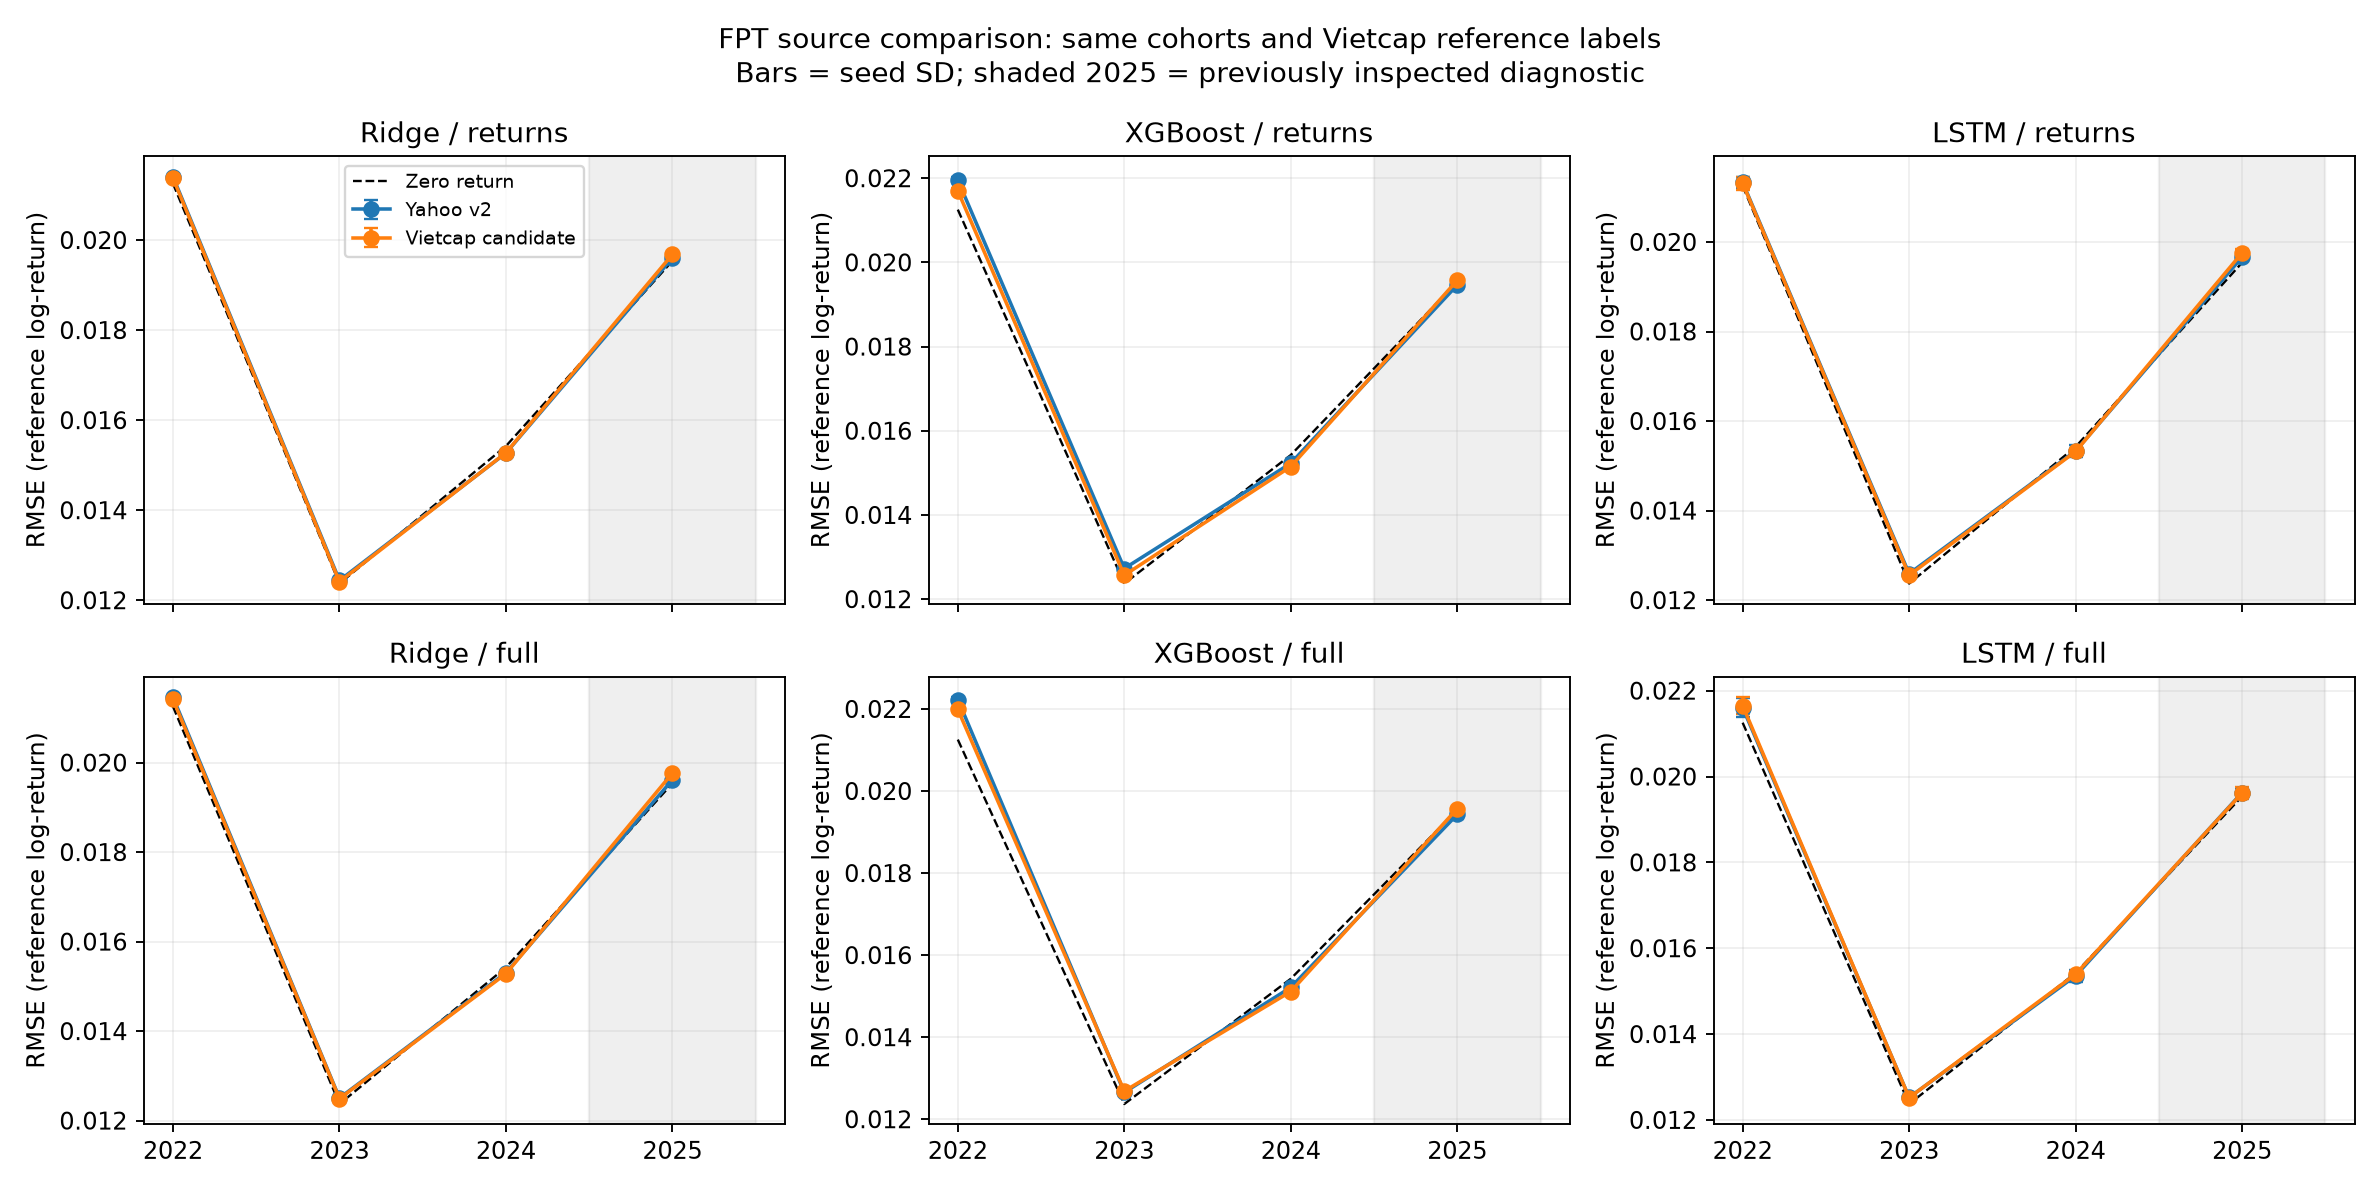
\includegraphics[width=0.92\textwidth]{06_source_comparison.png}
    \caption{Đối chiếu kết quả thực nghiệm của 112 cấu hình mô hình giữa nguồn dữ liệu Yahoo Finance (v2) và Vietcap (v3).}
    \label{fig:ch2_source_comparison}
\end{figure}

Từ Bảng~\ref{tab:ch2_audit} và Hình~\ref{fig:ch2_source_comparison}, nhóm chọn Vietcap thay cho Yahoo Finance vì các nguyên nhân sau:
\begin{itemize}
    \item Nguồn Yahoo Finance có tới \textbf{147 dòng khối lượng bằng 0} (phần lớn rơi vào các ngày nghỉ lễ Việt Nam bị giữ lại giá đóng cửa cũ), \textbf{4 dòng thiếu giá Close} và \textbf{1 cây nến sai lệch hình học} vào ngày 02/11/2021. Các dòng \texttt{Volume = 0} tạo ra hàng loạt nhãn giả $y_t = 0$, làm sai lệch phân phối lợi suất và độ chính xác hướng.
    \item Nguồn \textbf{Vietcap} (thu thập thông qua endpoint \texttt{POST https://trading.vietcap.com.vn/api/chart/OHLCChart/gap-chart}) đạt độ sạch gần như tuyệt đối với 1.997/1.999 phiên có khối lượng dương đến hết 2025, 0 thiếu Close và 0 nến lỗi.
    \item Nhóm chọn \textbf{Vietcap} làm nguồn dữ liệu chính thức cho toàn bộ nghiên cứu nâng cao và đóng gói sản phẩm đến ngày \textbf{29/10/2026}, đồng thời vẫn bảo lưu snapshot Yahoo v2 để đối chứng công bằng với mô hình LSTM lịch sử.
\end{itemize}

\section{Phân tích thống kê mô tả chuỗi dữ liệu Vietcap FPT (2018 -- 10/2026)}
Sau khi làm sạch và lọc bỏ các phiên khối lượng không dương trên snapshot Vietcap đến ngày 29/10/2026, tập dữ liệu chuẩn hóa gồm \textbf{2.200 phiên giao dịch hợp lệ} (từ ngày 02/01/2018 đến 29/10/2026), tương ứng với \textbf{2.199 quan sát tỷ suất sinh lời logarit ngày}. Thống kê mô tả toàn kỳ và theo từng năm được trình bày tại Bảng~\ref{tab:ch2_descriptive}.

\begin{table}[H]
\centering
\caption{Thống kê mô tả giá đóng cửa điều chỉnh và biến động hàng năm của cổ phiếu FPT (Nguồn Vietcap)}
\label{tab:ch2_descriptive}
\renewcommand{\arraystretch}{1.18}
\small
\setlength{\tabcolsep}{4.5pt}%
\resizebox{\ifdim\width>\textwidth\textwidth\else\width\fi}{!}{%
\begin{tabular}{@{}l r r r r r@{}}
\toprule
\textbf{Giai đoạn} & \textbf{Số phiên ($n$)} & \textbf{Giá đầu kỳ (VNĐ)} & \textbf{Giá cuối kỳ (VNĐ)} & \textbf{Biến động năm (\%)} & \textbf{Mean Return / ngày} \\
\midrule
Năm 2018 & 248 & 14.026 & 11.950 & 29,33\% & $-0,0648\%$ \\
Năm 2019 & 250 & 11.667 & 18.888 & 20,10\% & $+0,1831\%$ \\
Năm 2020 & 252 & 18.985 & 22.910 & 29,93\% & $+0,0766\%$ \\
Năm 2021 & 250 & 23.336 & 42.330 & 29,33\% & $+0,2456\%$ \\
Năm 2022 & 249 & 42.558 & 42.879 & \textbf{33,44\%} & $+0,0052\%$ \\
Năm 2023 & 249 & 44.607 & 63.068 & \textbf{19,89\%} & $+0,1550\%$ \\
Năm 2024 & 250 & 62.937 & 116.694 & 24,14\% & $+0,2461\%$ \\
Năm 2025 & 249 & 116.312 & 85.907 & 30,96\% & $-0,1230\%$ \\
Năm 2026 (đến 29/10) & 203 & 85.190 & 52.700 & \textbf{31,72\%} & $-0,2407\%$ \\
\midrule
\textbf{Toàn kỳ (2018--2026)} & \textbf{2.200} & \multicolumn{4}{l}{Min: $10.736,65$ (12/07/2018) \;|\; Max: $118.071,88$ (23/01/2025) \;|\; Std ngày: $1,765\%$} \\
\bottomrule
\end{tabular}%
}
\end{table}

Từ số liệu thực tế trên 2.199 quan sát log return, hai đặc trưng phân phối rất đáng chú ý được rút ra:
\begin{itemize}
    \item \textbf{Phân phối đuôi dày (Leptokurtic) và lệch trái nhẹ:} Chuỗi lợi suất có giá trị nhỏ nhất $-0,072476$ (giảm sàn $-7\%$), lớn nhất $+0,067627$ (tăng trần $+7\%$), độ lệch (Skewness) bằng $-0,0766$ và độ nhọn dư (\textbf{Excess Kurtosis}) bằng \textbf{$+2,8128$}. Đặc tính đuôi dày này là lý do nhóm chọn \textbf{Huber Loss} khi huấn luyện LSTM và dùng \textbf{Circular Block Bootstrap} thay cho giả định phân phối chuẩn $\pm 1,28\sigma$ khi ước lượng vùng bất định.
    \item \textbf{Sự luân chuyển chế độ thị trường (Regime Shift) giải thích biến động sai số giữa các năm:} Năm 2023 có biến động năm thấp nhất toàn chuỗi ($19,89\%$) và xu hướng tăng êm đềm, nên mọi mô hình ở Chương 4 đều đạt RMSE cực thấp quanh $0,0124$. Ngược lại, năm 2022 ($33,44\%$) và giai đoạn đảo chiều giảm 2025--2026 ($30,96\%$ -- $31,72\%$, mean return âm $-0,2407\%$/ngày) đẩy mức RMSE nền lên ngưỡng $0,020 - 0,021$. Đặc biệt, sự đảo dấu lợi suất trung bình từ dương mạnh ($+0,246\%$/ngày năm 2024) sang âm ($-0,241\%$/ngày năm 2026) là nguyên nhân gốc rễ khiến các mô hình đóng băng từ 2023 bị sai lệch dương và cần đến thành phần hiệu chỉnh nhân quả \texttt{bias60}.
\end{itemize}

\section{Quy tắc làm sạch, kiểm tra nến và cách ly lỗi (Quarantine)}
Mọi tập dữ liệu đầu vào trước khi trích xuất đặc trưng đều phải đi qua bộ lọc kiểm định hợp đồng dữ liệu (\texttt{src/data/}) với ba chốt chặn bắt buộc:
\begin{enumerate}
    \item \textbf{Cách ly dữ liệu khuyết và phiên không thanh khoản:} Các hàng chứa giá trị \texttt{NaN}/\texttt{Inf}, giá $\le 0$ hoặc $\text{Volume} \le 0$ được tách ra khỏi luồng tính toán và lưu vào danh sách cách ly (\nolinkurl{excluded_rows.csv}) để kiểm tra truy vết.
    \item \textbf{Kiểm tra ràng buộc hình học của nến OHLC:} Mọi phiên giao dịch hợp lệ bắt buộc phải thỏa mãn:
    \begin{equation}
        0 < \text{Low}_t \le \min(\text{Open}_t, \text{Close}_t) \le \max(\text{Open}_t, \text{Close}_t) \le \text{High}_t
    \end{equation}
    Các nến vi phạm (như ngày 02/11/2021 trên nguồn Yahoo) bị loại bỏ hoàn toàn; mọi nhãn $y$ trỏ vào ngày lỗi đó cũng bị hủy để tránh học từ dữ liệu méo.
    \item \textbf{Không điền khuyết giả tạo (No Forward-Fill):} Không dùng kỹ thuật \texttt{ffill} chép giá vào ngày lễ hoặc cuối tuần. Phiên tiếp theo $\text{next}(t)$ được định nghĩa chặt chẽ là quan sát có khối lượng dương hợp lệ liền sau ngày $t$. Dữ liệu sử dụng hệ quy chiếu giá điều chỉnh của nhà cung cấp (\nolinkurl{provider_adjusted_ohlc}, \texttt{point\_in\_time\_certified = false}).
\end{enumerate}

\section{Kỹ thuật tạo đặc trưng và Thực nghiệm thu gọn đặc trưng}

\subsection{Bộ 16 đặc trưng đầy đủ ở giai đoạn nghiên cứu khởi đầu (Pipeline v2)}
Ở giai đoạn đầu (\nolinkurl{src/features/build_features.py}), nhóm xây dựng bộ \textbf{16 đặc trưng kỹ thuật nhân quả} nhằm cung cấp cho mạng LSTM, XGBoost và Ridge bức tranh đa chiều về xu hướng, động lượng, độ biến động và dòng tiền (Bảng~\ref{tab:ch2_features_16}). Do chỉ báo \nolinkurl{SMA_Distance_50} yêu cầu tối thiểu 50 phiên để tính trung bình trượt, \textbf{49 quan sát đầu tiên} của chuỗi được dành làm giai đoạn khởi động (\textit{warm-up}) nhằm loại bỏ hoàn toàn giá trị thiếu.

\begin{table}[H]
\centering
\caption{Danh mục 16 đặc trưng nhân quả trong giai đoạn Pipeline v2}
\label{tab:ch2_features_16}
\renewcommand{\arraystretch}{1.15}
\small
\setlength{\tabcolsep}{4.5pt}%
\resizebox{\ifdim\width>\textwidth\textwidth\else\width\fi}{!}{%
\begin{tabular}{@{}l >{\ttfamily}l p{8.4cm}@{}}
\toprule
\textbf{Nhóm} & \normalfont\textbf{Tên đặc trưng} & \textbf{Công thức và ý nghĩa kỹ thuật tại đóng cửa ngày $t$} \\
\midrule
\multirow{6}{*}{Lợi suất (6)} & Log\_Return & $\ln(C_t / C_{t-1})$: Tỷ suất sinh lời logarit phiên hiện tại. \\
 & Return\_Lag\_1 & Lợi suất logarit trễ 1 phiên ($y_{t-1}$). \\
 & Return\_Lag\_2 & Lợi suất logarit trễ 2 phiên ($y_{t-2}$). \\
 & Return\_Lag\_5 & Lợi suất logarit trễ 5 phiên (1 tuần giao dịch trước). \\
 & Return\_5 & $\ln(C_t / C_{t-5})$: Lợi suất tích lũy ngắn hạn trong 5 phiên. \\
 & Return\_20 & $\ln(C_t / C_{t-20})$: Lợi suất tích lũy trung hạn trong 20 phiên ($\approx 1$ tháng). \\
\midrule
\multirow{2}{*}{Biến động (2)} & Volatility\_5 & Độ lệch chuẩn trượt của \nolinkurl{Log_Return} trong 5 phiên. \\
 & Volatility\_20 & Độ lệch chuẩn trượt của \nolinkurl{Log_Return} trong 20 phiên. \\
\midrule
\multirow{2}{*}{Xu hướng (2)} & SMA\_Distance\_20 & $(C_t - \text{SMA}_{20}(C)_t) / \text{SMA}_{20}(C)_t$: Độ lệch tương đối so với MA20. \\
 & SMA\_Distance\_50 & $(C_t - \text{SMA}_{50}(C)_t) / \text{SMA}_{50}(C)_t$: Độ lệch tương đối so với MA50. \\
\midrule
Động lượng & RSI\_14 & Chỉ số sức mạnh tương đối Wilder (Relative Strength Index 14 phiên). \\
\midrule
\multirow{2}{*}{Biên độ (2)} & ATR\_Ratio & $\text{ATR}_{14, t} / C_t$: Biên độ dao động thực tế chuẩn hóa theo mức giá. \\
 & Intraday\_Range & $(H_t - L_t) / C_t$: Biên độ dao động nội phiên ngày $t$. \\
\midrule
\multirow{3}{*}{Khối lượng (3)} & Volume\_Ratio\_20 & $V_t / \text{SMA}_{20}(V)_t$: Tỷ số thanh khoản so với trung bình 20 phiên. \\
 & Volume\_Log\_Change & $\ln(V_t / V_{t-1})$: Tốc độ biến thiên khối lượng theo logarit. \\
 & Volume\_ZScore\_20 & $(V_t - \mu_{V,20}) / \sigma_{V,20}$: Điểm chuẩn hóa Z-score của thanh khoản. \\
\bottomrule
\end{tabular}%
}
\end{table}

\subsection{Thu gọn về bộ 6 đặc trưng lợi suất cốt lõi (\texttt{Ridge6})}
Khi tiến hành Đợt huấn luyện 2 (\textit{Robustness Study} với 63 cấu hình) và Đợt huấn luyện 4 (\textit{Window Comparison}), nhóm nhận thấy đưa đồng thời 16 chỉ báo kỹ thuật vào mô hình trên tập mẫu ngày vốn có tỷ lệ nhiễu lớn gây hiện tượng quá khớp (overfitting) nghiêm trọng. Các chỉ báo phụ thuộc mức giá hoặc khối lượng như \nolinkurl{SMA_Distance_50}, \texttt{RSI\_14}, \nolinkurl{Volume_ZScore_20} chứa đa cộng tuyến cao và mất tính ổn định khi cổ phiếu đổi xu hướng.

Bằng phép loại bỏ đặc trưng có kiểm chứng (Feature Pruning), nhóm rút gọn không gian đầu vào về \textbf{đúng 6 đặc trưng lợi suất thuần túy (Returns-Only)}:
\begin{equation}
    \mathbf{x}_t^{(6)} = \big[\texttt{Log\_Return},\; \texttt{Return\_Lag\_1},\; \texttt{Return\_Lag\_2},\; \texttt{Return\_Lag\_5},\; \texttt{Return\_5},\; \texttt{Return\_20}\big]^\top \in \mathbb{R}^6
\end{equation}
Việc tinh giản xuống 6 đặc trưng này mang lại ba lợi ích chính: (1) loại bỏ nhiễu đa cộng tuyến của các chỉ báo kỹ thuật; (2) đảm bảo tính bất biến theo thang đo giá tuyệt đối qua suốt 8 năm lịch sử; và (3) cho phép hệ thống chỉ cần đúng \textbf{21 giá đóng cửa gần nhất} là có thể vận hành vòng lặp mô phỏng đa bước đệ quy mà không phải tự tạo giả giá Open, High, Low hay Volume tương lai. Lưu ý kỹ thuật: để giữ nguyên mốc thời gian so sánh công bằng với Pipeline 16 đặc trưng, bộ tạo đặc trưng chuẩn vẫn khởi động sau 49 phiên đầu tiên.

\subsection{Thực nghiệm A/B tách nhảy giá qua đêm (Gap) và thân nến (Body)}
Ở Đợt huấn luyện 7 (\textit{Candle Ablation Study} mã \texttt{20261030T\-093521684942Z}), nhóm đặt giả thuyết tách lợi suất ngày hiện tại thành hai yếu tố phản ánh tâm lý nhà đầu tư: nhảy giá qua đêm do tin tức (\textit{Overnight Gap}) và biến động cung cầu trong phiên (\textit{Intraday Body}):
\begin{equation}
    \text{Gap}_t = \ln\left(\frac{\text{Open}_t}{\text{Close}_{\text{prev}(t)}}\right), \qquad \text{Body}_t = \ln\left(\frac{\text{Close}_t}{\text{Open}_t}\right)
\end{equation}
Vì $\text{Gap}_t + \text{Body}_t = \text{Log\_Return}_t$, nhánh B thay thế \nolinkurl{Log_Return} bằng cặp $(\text{Gap}_t, \text{Body}_t)$ (tạo thành bộ \nolinkurl{B_gap_body7}, tránh đa cộng tuyến hoàn hảo) và chạy đối chứng 20 lượt fit mới với 20 mô hình nhánh A.

\begin{figure}[H]
    \centering
    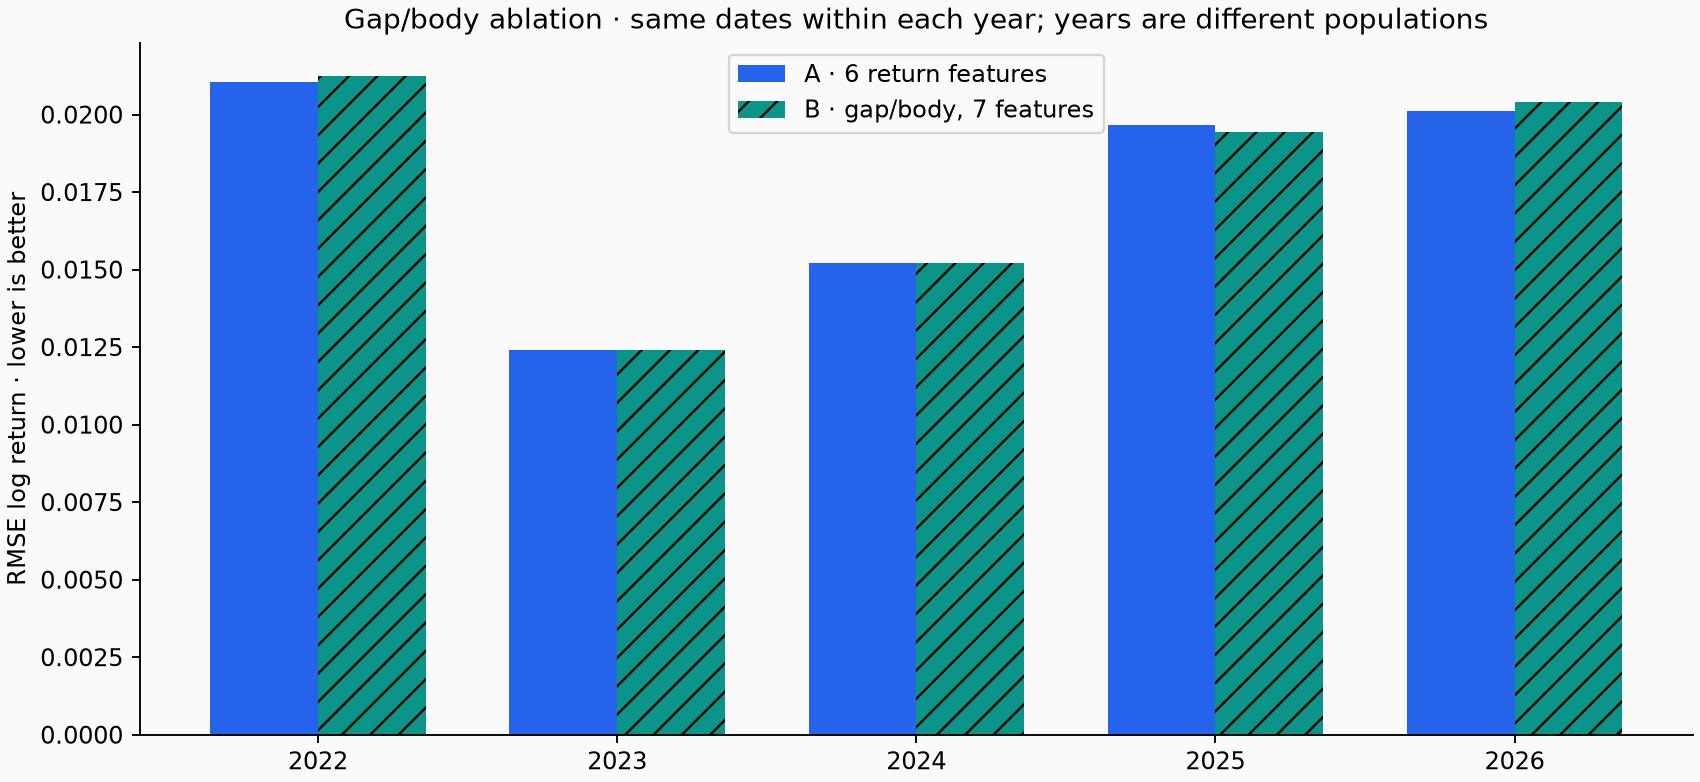
\includegraphics[width=0.92\textwidth]{02_gap_body.png}
    \caption{Thực nghiệm đối chứng A/B theo từng năm giữa bộ 6 đặc trưng lợi suất gốc (A) và bộ 7 đặc trưng tách Gap/Body (B).}
    \label{fig:ch2_gap_body}
\end{figure}

Như minh họa tại Hình~\ref{fig:ch2_gap_body}, dù nhánh B có nhỉnh hơn ở một vài năm cá biệt, nhưng tính trung bình trên giai đoạn chính 2022--2024, \nolinkurl{Ridge_recent} bị tăng RMSE từ $0,0162190$ (nhánh A) lên $0,0162930$ (nhánh B, tăng $0,46\%$). Trên tập 202 phiên năm 2026, nhánh B làm RMSE của Ridge tăng từ $0,0201191$ lên $0,0204083$ và kéo Hit Rate tụt mạnh từ $50,76\%$ xuống $44,67\%$. Do không mang lại lợi ích ổn định, nhóm bác bỏ nhánh B và giữ nguyên bộ 6 đặc trưng lợi suất A.

\section{Chiến lược chia tập dữ liệu và chống rò rỉ (Zero-Leakage Protocol)}
Hệ thống khóa cứng bốn nguyên tắc bảo vệ tính nhân quả trong mọi thí nghiệm:

\begin{enumerate}
    \item \textbf{Tuyệt đối không chia ngẫu nhiên (No Random Split):} Dữ liệu luôn bảo toàn trật tự thời gian tăng dần.
    \item \textbf{Chốt chặn ranh giới ngày đích (\textit{Target Date Boundary Purging}):} Với mỗi mốc cắt tập Train $T_{\text{cutoff}}$ (như 31/12/2022 hoặc 31/12/2025), một mẫu tại ngày $t$ chỉ được phép tham gia vào tập Train khi thỏa mãn đồng thời:
    \begin{equation}
        \text{Date}_t \le T_{\text{cutoff}} \quad \textbf{VÀ} \quad \text{Target\_Date\_1d}_t \le T_{\text{cutoff}}
    \end{equation}
    Mọi phiên cuối năm có ngày giao dịch kế tiếp vắt sang đầu năm Validation sẽ bị loại khỏi tập Train để ngăn thông tin năm sau rò rỉ vào quá trình khớp trọng số. Trong khi đó, đối với tập Validation và Test, mô hình LSTM vẫn được phép truy xuất 30 ngày lịch sử trước ngày gốc đầu tiên vì toàn bộ lịch sử đó đã hoàn tất trước thời điểm dự báo.
    \item \textbf{Chuẩn hóa độc lập theo tập Train (\textit{Train-Only Scaling}):} Các bộ chuẩn hóa \texttt{StandardScaler} hoặc \texttt{MinMaxScaler} chỉ gọi \texttt{.fit()} duy nhất trên tập Train của từng fold, sau đó dùng thống kê cố định để \nolinkurl{.transform()} các tập sau.
    \item \textbf{Đánh giá cuốn chiếu (\textit{Walk-Forward Validation}) \cite{hyndman2021fpp3,lopez2018afml}:} Quá trình chọn tham số không dựa vào một lần chia duy nhất mà được lặp cuốn chiếu qua 4 năm liên tiếp (2022, 2023, 2024, 2025), mỗi năm huấn luyện độc lập một mô hình mới tính đến hết 31/12 của năm liền trước (Hình~\ref{fig:ch2_walkforward}).
\end{enumerate}

\begin{figure}[H]
\centering
\begin{tikzpicture}[scale=0.88, every node/.style={font=\small}]
    % Trục thời gian
    \draw[->, thick, color=primaryblue] (0, 3.8) -- (13.8, 3.8) node[right] {\textbf{Thời gian}};
    \foreach \x/\lbl in {0.5/2019, 2.8/2020, 5.1/2021, 7.4/2022, 9.5/2023, 11.4/2024, 13.0/2025} {
        \draw (\x, 3.7) -- (\x, 3.9) node[above=2pt] {\lbl};
    }

    % Fold 2022 (3y: 2019-2021 -> eval 2022)
    \node[left] at (0.3, 2.8) {\textbf{Fold 2022}};
    \fill[primaryblue!25] (0.5, 2.55) rectangle (7.2, 3.05);
    \draw[primaryblue] (0.5, 2.55) rectangle (7.2, 3.05) node[pos=0.5, text=primaryblue] {Train 3 năm (2019--2021)};
    \fill[red!40] (7.2, 2.55) rectangle (7.4, 3.05);
    \fill[accentteal!30] (7.4, 2.55) rectangle (9.5, 3.05);
    \draw[accentteal] (7.4, 2.55) rectangle (9.5, 3.05) node[pos=0.5, text=accentteal!80!black] {Eval 2022};

    % Fold 2023
    \node[left] at (0.3, 2.0) {\textbf{Fold 2023}};
    \fill[primaryblue!25] (2.8, 1.75) rectangle (9.3, 2.25);
    \draw[primaryblue] (2.8, 1.75) rectangle (9.3, 2.25) node[pos=0.5, text=primaryblue] {Train 3 năm (2020--2022)};
    \fill[red!40] (9.3, 1.75) rectangle (9.5, 2.25);
    \fill[accentteal!30] (9.5, 1.75) rectangle (11.4, 2.25);
    \draw[accentteal] (9.5, 1.75) rectangle (11.4, 2.25) node[pos=0.5, text=accentteal!80!black] {Eval 2023};

    % Fold 2024
    \node[left] at (0.3, 1.2) {\textbf{Fold 2024}};
    \fill[primaryblue!25] (5.1, 0.95) rectangle (11.2, 1.45);
    \draw[primaryblue] (5.1, 0.95) rectangle (11.2, 1.45) node[pos=0.5, text=primaryblue] {Train 3 năm (2021--2023)};
    \fill[red!40] (11.2, 0.95) rectangle (11.4, 1.45);
    \fill[accentteal!30] (11.4, 0.95) rectangle (13.0, 1.45);
    \draw[accentteal] (11.4, 0.95) rectangle (13.0, 1.45) node[pos=0.5, text=accentteal!80!black] {Eval 2024};

    % Fold 2025
    \node[left] at (0.3, 0.4) {\textbf{Fold 2025}};
    \fill[primaryblue!25] (7.4, 0.15) rectangle (12.8, 0.65);
    \draw[primaryblue] (7.4, 0.15) rectangle (12.8, 0.65) node[pos=0.5, text=primaryblue] {Train 3 năm (2022--2024)};
    \fill[red!40] (12.8, 0.15) rectangle (13.0, 0.65);
    \fill[accentteal!30] (13.0, 0.15) rectangle (14.4, 0.65);
    \draw[accentteal] (13.0, 0.15) rectangle (14.4, 0.65) node[pos=0.5, text=accentteal!80!black] {Eval 2025};

    % Chú thích vùng Purge
    \fill[red!40] (0.5, -0.45) rectangle (0.9, -0.15);
    \node[right] at (1.0, -0.3) {\footnotesize Vùng chốt chặn biên (\textit{Boundary Purge}): loại bỏ mẫu có \texttt{Target\_Date\_1d} vượt qua ngày 31/12 năm cắt.};
\end{tikzpicture}
\caption{Cơ chế kiểm định Walk-Forward 4 năm với cửa sổ trượt 3 năm và chốt chặn biên chống rò rỉ nhãn.}
\label{fig:ch2_walkforward}
\end{figure}

% ==========================================
% CHƯƠNG 3: CÁC MÔ HÌNH THỰC NGHIỆM TRONG DỰ ÁN
% ==========================================
\chapter{Các mô hình thực nghiệm trong dự án}

Nhóm triển khai và so sánh năm nhóm thuật toán từ các đường cơ sở thống kê đơn giản đến mô hình tuyến tính điều chuẩn, cây tăng cường gradient, mạng học sâu chuỗi thời gian và phân loại xác suất.

\section{Nhóm mô hình cơ sở (Mandatory Baselines)}
Mọi mô hình Học máy trong dự án bắt buộc phải chứng minh giá trị trước năm đường cơ sở sau trên cùng tập ngày gốc và nhãn đích:
\begin{enumerate}
    \item \textbf{Zero-Return ($\hat{y}_t = 0$):} Mô hình bước đi ngẫu nhiên (Random Walk), giả định giá đóng cửa ngày mai bằng đúng giá hôm nay. Vì không phát tín hiệu biến động, chỉ số Hit Rate và Balanced Accuracy được ghi là \texttt{N/A}. Đây là chuẩn đối chiếu quan trọng nhất về sai số dự báo độ lớn (RMSE, MAE).
    \item \textbf{Train Mean ($\hat{y}_t = \bar{y}_{\text{train}}$):} Dự báo lợi suất phiên tới luôn bằng trung bình cộng lợi suất trong tập huấn luyện. Dù đơn giản, \texttt{Train Mean} thường rất khó bị đánh bại khi chuỗi dữ liệu có nhiễu lớn.
    \item \textbf{Return Persistence ($\hat{y}_t = y_{t-1}$):} Giả định phiên tới lặp lại đúng lợi suất của phiên vừa đóng cửa. Trên thực tế chứng khoán Việt Nam, lợi suất ngày thường có hiện tượng đảo chiều nhẹ (mean-reversion), nên mô hình này thường có sai số cao gấp rưỡi \nolinkurl{Zero-Return}.
    \item \textbf{Always Up / Always Down:} Hai mô hình hằng số luôn đoán Tăng hoặc luôn đoán Giảm, được dùng để phát hiện ảo giác Hit Rate cao khi thị trường mất cân bằng số phiên tăng/giảm.
\end{enumerate}

\section{Hồi quy Tuyến tính và Điều chuẩn Ridge $L_2$ kết hợp \texttt{bias60}}

\subsection{Mô hình Linear Regression và Ridge Regression ($L_2$ Regularization)}
Mô hình Hồi quy Tuyến tính thông thường (OLS) có xu hướng khuếch đại nhiễu khi các đặc trưng lợi suất trễ mang nhiều dao động ngẫu nhiên. Mô hình \textbf{Ridge Regression} \cite{hoerl1970ridge,pedregosa2011sklearn} khắc phục nhược điểm này bằng cách bổ sung thành phần phạt chuẩn bình phương $L_2$ lên vector trọng số $\mathbf{w} \in \mathbb{R}^d$:
\begin{equation}
    \min_{\mathbf{w}, b} \sum_{i=1}^{N_{\text{train}}} \left(y_i - (\mathbf{w}^\top \tilde{\mathbf{x}}_i + b)\right)^2 + \alpha \|\mathbf{w}\|_2^2
    \label{eq:ch3_ridge}
\end{equation}
trong đó $\tilde{\mathbf{x}}_i = (\mathbf{x}_i - \boldsymbol{\mu}_{\text{train}}) \oslash \boldsymbol{\sigma}_{\text{train}}$ là đặc trưng đã chuẩn hóa bằng \texttt{StandardScaler} chỉ khớp trên tập Train, còn $\alpha > 0$ kiểm soát cường độ co trọng số (shrinkage). Nghiệm tối ưu có dạng đóng duy nhất:
\begin{equation}
    \hat{\mathbf{w}} = \left(\tilde{\mathbf{X}}^\top \tilde{\mathbf{X}} + \alpha \mathbf{I}\right)^{-1} \tilde{\mathbf{X}}^\top (\mathbf{y} - \bar{y})
\end{equation}
Khi $\alpha$ lớn (như $\alpha = 100$ được tìm ra qua thực nghiệm ở Chương 4), thuật toán ép mạnh các hệ số nhỏ và triệt tiêu phương sai ngoài mẫu, giúp đường dự báo không phản ứng thái quá trước các cú giật cục đơn lẻ.

\subsection{Hiệu chỉnh độ chệch nhân quả trượt 60 phiên (\texttt{Ridge+bias60})}
Trong tài chính thực tế, mô hình Ridge huấn luyện trên cửa sổ 3 năm thường mang kỳ vọng trung bình dài hạn ($\hat{b} \approx \bar{y}_{3y}$). Khi cổ phiếu chuyển sang một chu kỳ điều chỉnh kéo dài vài tháng (như năm 2026), dự báo thô $\hat{y}_t^{\text{raw}}$ liên tục cao hơn thực tế một lượng lệch hệ thống. Để thích nghi mà không phải tính lại trọng số ma trận mỗi ngày, nhóm bổ sung thành phần \textbf{hiệu chỉnh độ chệch nhân quả trượt (\texttt{bias60})}:
\begin{equation}
    \text{bias}_{60}(t) = \frac{1}{|S_t|} \sum_{k \in S_t} \left(y_k - \hat{y}_k^{\text{raw}}\right), \qquad S_t = \big\{k : \text{Target\_Date\_1d}(k) \le t,\; \text{tối đa } 60 \text{ mẫu gần nhất}\big\}
\end{equation}
Điều kiện $\text{Target\_Date\_1d}(k) \le t$ (cùng yêu cầu tối thiểu 20 mẫu trưởng thành) đảm bảo tại thời điểm phát dự báo sau đóng cửa ngày $t$, thuật toán \textbf{chỉ sử dụng những sai số quá khứ mà kết quả thực tế đã hoàn toàn ngã ngũ}. Dự báo một bước đã hiệu chỉnh được tính là $\hat{y}_t^{\text{cal}} = \hat{y}_t^{\text{raw}} + \text{bias}_{60}(t)$. Đối với phiên bản đóng gói local (\nolinkurl{ridge6_20261029}), vector 60 sai số thô và 60 sai số đã hiệu chỉnh đến ngày 29/10/2026 được đóng băng cố định trong tệp \nolinkurl{calibration.json}.

\section{Cây tăng cường Gradient (XGBoost) và Mạng học sâu (LSTM)}

\subsection{Mô hình XGBoost Regressor}
Để kiểm tra xem các tương tác phi tuyến dạng cây quyết định có mang lại lợi thế so với mô hình tuyến tính hay không, nhóm cấu hình \texttt{XGBRegressor} \cite{chen2016xgboost} với độ sâu cây giới hạn nông (\texttt{max\_depth = 2}, nhằm hạn chế học thuộc nhiễu trên tập mẫu nhỏ) trong Pipeline v2 và toàn bộ các đợt nghiên cứu Robustness / Window Comparison. Toàn bộ mô hình XGBoost được lưu dưới định dạng JSON chuẩn của thư viện để bảo đảm tính tái lập giữa Windows CPU và Linux GPU.

\subsection{Mạng nơ-ron hồi quy LSTM (Long Short-Term Memory)}
Nhóm xây dựng mô hình Học sâu LSTM \cite{hochreiter1997lstm} trong \nolinkurl{src/models/experiment.py} và notebook \nolinkurl{02_train_deep_learning_fpt.ipynb} nhằm đánh giá khả năng khai thác phụ thuộc chuỗi dài hạn trên bộ 16 đặc trưng kỹ thuật:
\begin{itemize}
    \item \textbf{Dữ liệu đầu vào 3 chiều:} Tensor kích thước $(N, L, 16)$ ghép trượt từ $L$ phiên giao dịch liên tiếp trước ngày gốc $t$. Nhóm thực hiện \textbf{Ablation Study} trên ba chiều dài cửa sổ trượt $L \in \{10, 30, 60\}$ phiên.
    \item \textbf{Kiến trúc mạng nơ-ron v2:}
    \begin{center}
        \texttt{Input(L, 16)} $\longrightarrow$ \texttt{LSTM(32 units)} $\longrightarrow$ \texttt{Dropout(0,2)} $\longrightarrow$ \texttt{Dense(8, ReLU)} $\longrightarrow$ \texttt{Dense(1, Linear)}
    \end{center}
    \item \textbf{Cấu hình tối ưu và chống Overfitting:} Sử dụng hàm mất mát \textbf{Huber Loss} \cite{huber1964robust} (kết hợp tính mượt của MSE quanh 0 và tính bền vững của MAE trước các phiên trần/sàn đuôi dày), bộ tối ưu \textbf{Adam} ($\text{lr} = 0,001$, \texttt{clipnorm = 1.0}), \texttt{batch\_size = 32}, \texttt{shuffle = False} để giữ trật tự chuỗi, giới hạn tối đa 40 epochs kèm \texttt{EarlyStopping(patience=7)} và \texttt{ReduceLROnPlateau} theo dõi \texttt{val\_loss}.
\end{itemize}

\begin{figure}[H]
    \centering
    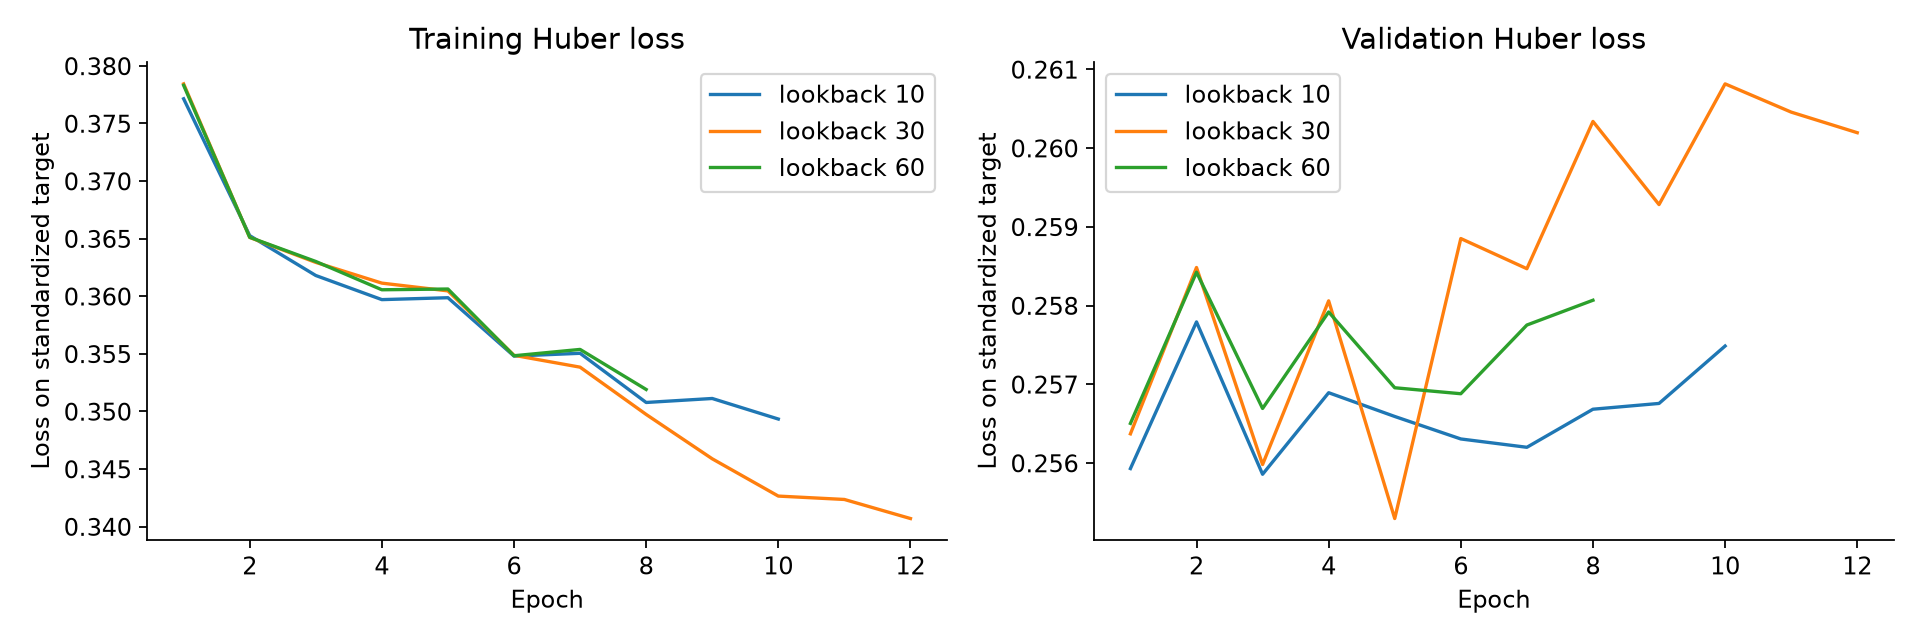
\includegraphics[width=0.92\textwidth]{04_lstm_learning_curves.png}
    \caption{Đường cong hàm mất mát Huber Loss trên tập Train và Validation theo từng epoch với các mức Lookback 10, 30 và 60 ngày.}
    \label{fig:ch3_lstm_curves}
\end{figure}

\begin{figure}[H]
    \centering
    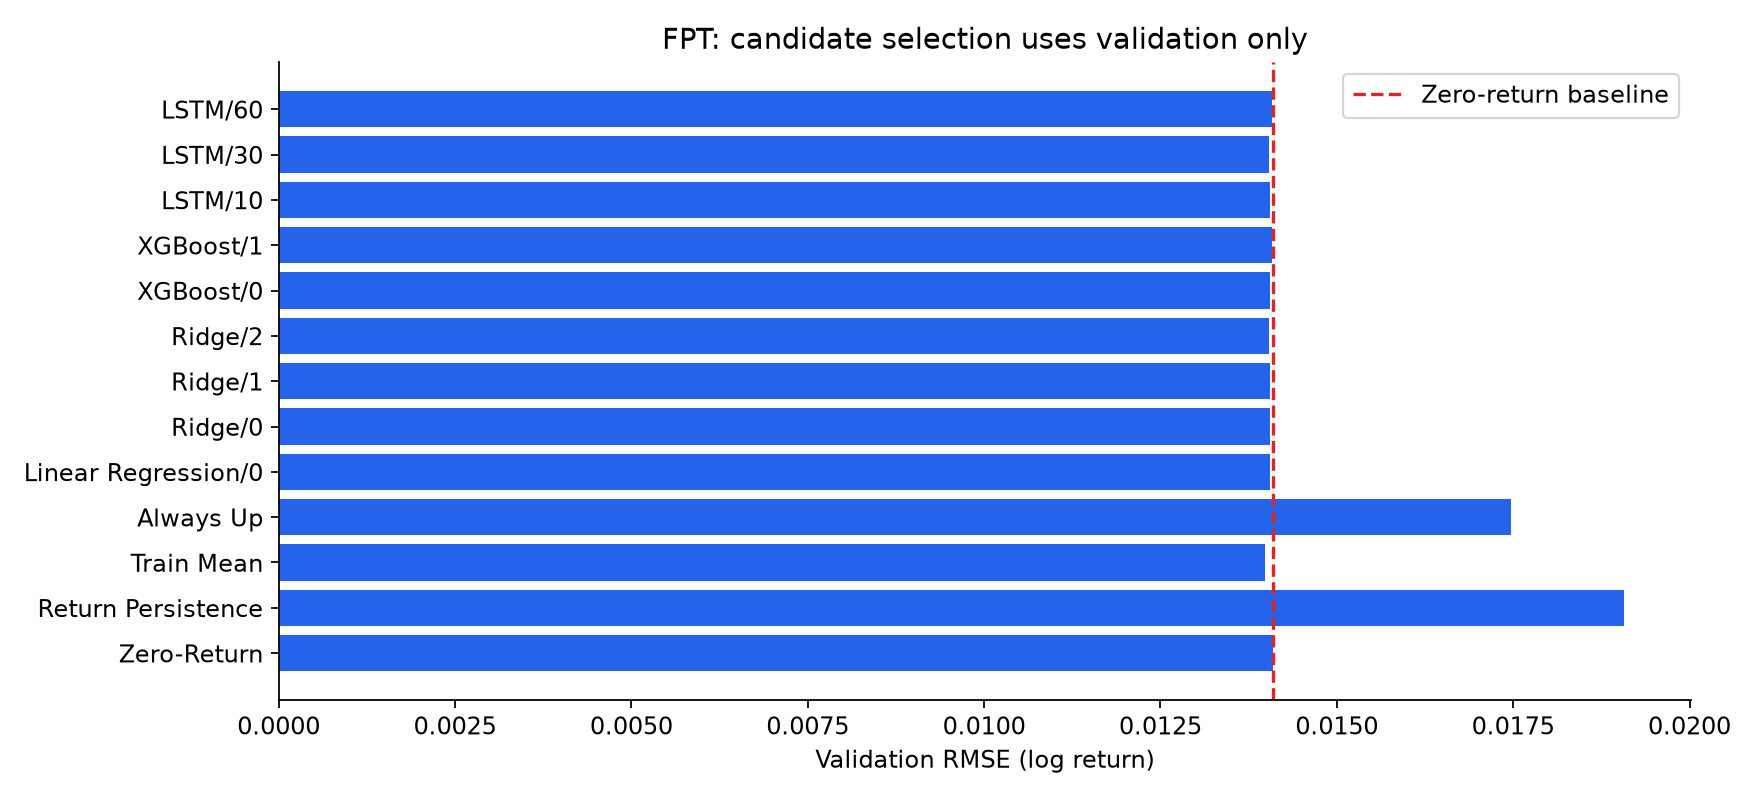
\includegraphics[width=0.90\textwidth]{11_lstm_lookback_ablation.png}
    \caption{Đối chứng lựa chọn độ dài cửa sổ trượt (Lookback = 10, 30, 60) của LSTM trên tập Validation.}
    \label{fig:ch3_lstm_ablation}
\end{figure}

\begin{table}[H]
\centering
\caption{Kết quả đối chứng 8 mô hình Pipeline v2 (Nguồn Yahoo, đối chứng CPU Reference)}
\label{tab:ch3_v2_benchmark}
\renewcommand{\arraystretch}{1.18}
\small
\setlength{\tabcolsep}{4.5pt}%
\resizebox{\ifdim\width>\textwidth\textwidth\else\width\fi}{!}{%
\begin{tabular}{@{}l r r r | r r r r@{}}
\toprule
\textbf{Mô hình} & \multicolumn{3}{c|}{\textbf{Validation (2023--2024, $n=493$)}} & \multicolumn{4}{c}{\textbf{Test Lịch sử (2025, $n=248$)}} \\
 & \textbf{RMSE $\downarrow$} & \textbf{MAE $\downarrow$} & \textbf{Hit (\%)} & \textbf{RMSE $\downarrow$} & \textbf{MAE $\downarrow$} & \textbf{Hit (\%)} & \textbf{Skill vs Zero} \\
\midrule
Zero-Return & 0,014095 & 0,010102 & N/A & 0,019917 & \textbf{0,013146} & N/A & 0,0000 \\
Return Persistence & 0,019069 & 0,014454 & 48,92 & 0,027995 & 0,021221 & 36,02 & $-0,9757$ \\
\textbf{Train Mean} & \textbf{0,013981} & 0,010076 & 54,74 & 0,020022 & 0,013429 & 45,02 & $-0,0105$ \\
Always Up & 0,017470 & 0,014261 & 54,74 & 0,024133 & 0,019055 & 45,02 & $-0,4682$ \\
\midrule
Linear Regression & 0,014051 & 0,010104 & 51,72 & 0,020080 & 0,013623 & 52,13 & $-0,0164$ \\
Ridge ($\alpha=10$) & 0,014035 & 0,010085 & 50,65 & 0,020055 & 0,013588 & 52,61 & $-0,0139$ \\
XGBoost (depth=2) & 0,014046 & 0,010060 & \textbf{56,03} & 0,020017 & 0,013807 & 43,13 & $-0,0101$ \\
\textbf{LSTM (lb=30)} & \textbf{0,014033} & \textbf{0,009997} & 54,74 & \textbf{0,019858} & 0,013442 & \textbf{54,98} & \textbf{+0,0059} \\
\bottomrule
\end{tabular}%
}
\end{table}

\begin{figure}[H]
    \centering
    \begin{subfigure}[b]{0.49\textwidth}
        \centering
        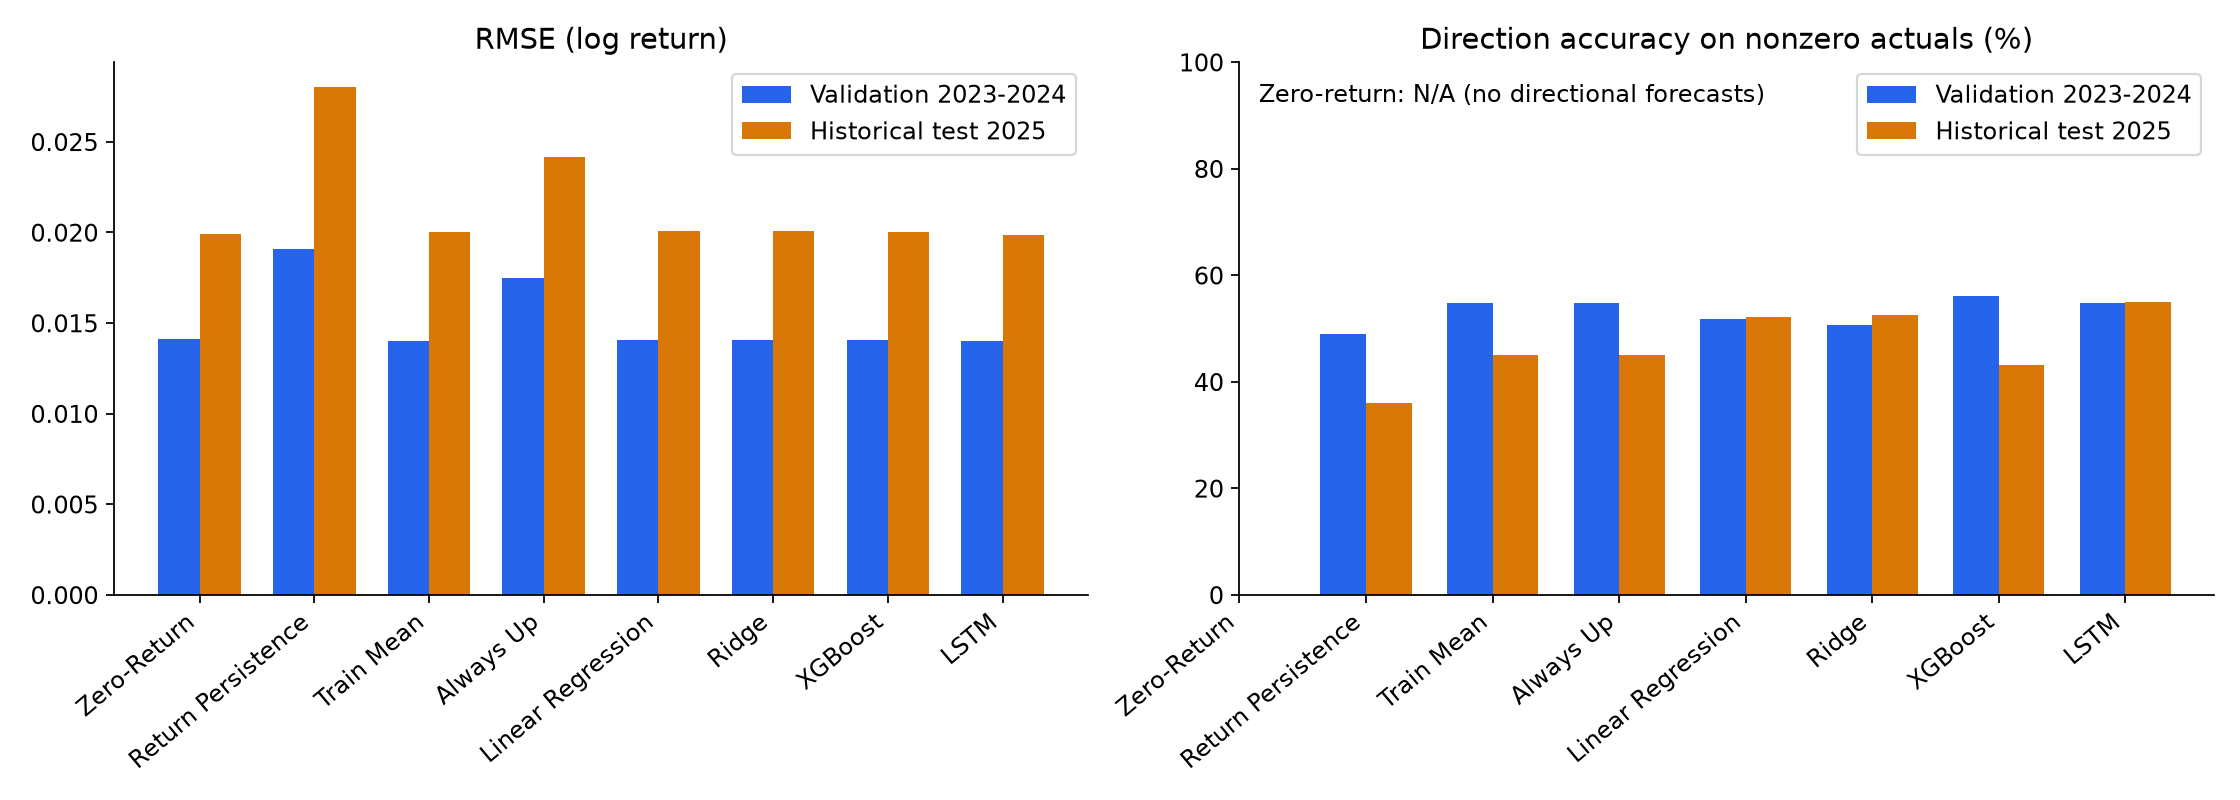
\includegraphics[width=\textwidth]{05_v2_benchmark.png}
        \caption{So sánh RMSE Validation và Test}
    \end{subfigure}
    \hfill
    \begin{subfigure}[b]{0.49\textwidth}
        \centering
        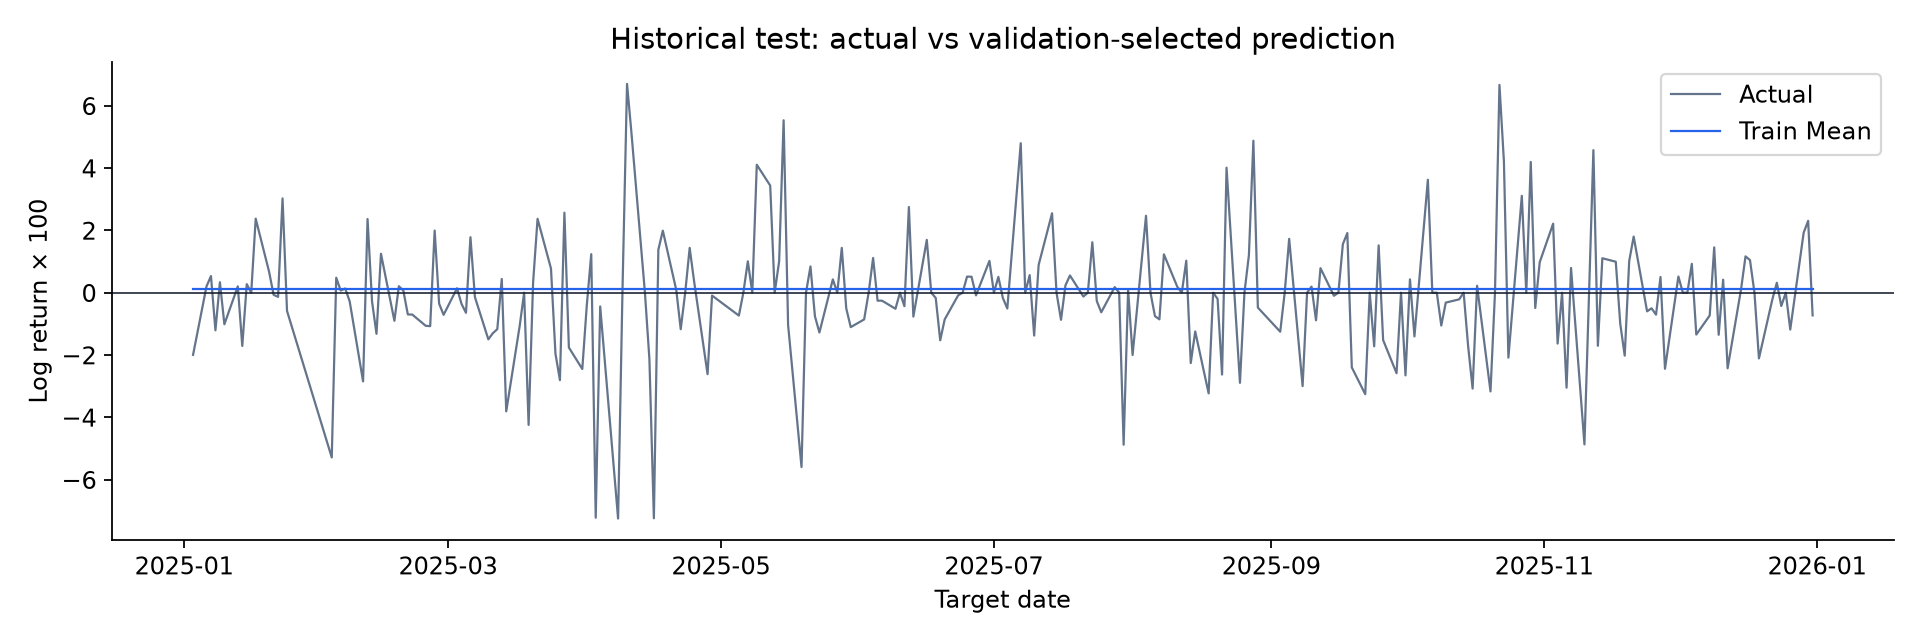
\includegraphics[width=\textwidth]{12_v2_test_returns.png}
        \caption{Dự báo vs thực tế trên tập Test 2025}
    \end{subfigure}
    \caption{Kết quả đối chứng toàn diện 8 mô hình ở Pipeline v2 (CPU Reference).}
    \label{fig:ch3_v2_pair}
\end{figure}

Khả năng tổng quát hóa của các mô hình ở Pipeline v2 được minh họa trực quan tại Hình~\ref{fig:ch3_v2_pair}. Từ Hình~\ref{fig:ch3_lstm_curves}, Hình~\ref{fig:ch3_lstm_ablation} và Bảng~\ref{tab:ch3_v2_benchmark}, có hai điểm rút ra then chốt:
\begin{enumerate}
    \item Trong nhóm LSTM, \texttt{LSTM30} đạt sai số Validation thấp nhất ($0,014033$) và dừng sớm ở epoch 12 (chạy lại trên Google Colab GPU A100 ở notebook 02 cũng xác nhận Lookback 30 đạt Val Hit Rate cao nhất $52,16\%$ so với $50,86\%$ của 10 ngày và $48,49\%$ của 60 ngày).
    \item Tuy nhiên, trên tập Validation 2023--2024, mô hình chiến thắng chung cuộc lại là hằng số \texttt{Train Mean} ($0,013981$). Và khi đánh giá lại các mô hình v2 trên dữ liệu sạch Vietcap năm 2026 (Chương 4), biên độ lợi thế của LSTM biến mất hoàn toàn. Đây chính là động lực khiến nhóm không vội kết luận sau lượt train đầu tiên mà tiếp tục mở rộng sang các vòng nghiên cứu đối chứng sâu hơn.
\end{enumerate}

\section{Nhánh Phân loại hướng và Dự báo có chọn lọc (Selective Classification)}
Nhằm kiểm tra xem liệu việc chuyển bài toán sang dự đoán xác suất Tăng/Giảm kết hợp từ chối các ngày không chắc chắn (\textit{Selective Abstain}) có hiệu quả hơn không, nhóm triển khai Đợt huấn luyện 6 (\textit{Direction Selective Study} mã \texttt{20261030T\-090621177786Z}) với 20 mô hình nền tảng và 10 bộ hiệu chỉnh xác suất. Hai thuật toán \textbf{Logistic Regression} và \textbf{XGBoost Classifier} được huấn luyện trên nhãn nhị phân $z_t = \mathbb{I}(y_t > 0)$, sau đó đưa qua bước hiệu chỉnh \textbf{Platt Sigmoid Calibration} \cite{platt1999probabilistic} để biến đổi điểm số thô thành xác suất $p_t \in [0, 1]$ và áp dụng ngưỡng biên $\tau$: nếu $|p_t - 0,5| < \tau$ thì hệ thống trả về trạng thái \nolinkurl{chua_du_tin_hieu}.

\begin{table}[H]
\centering
\caption{Kết quả nhánh Phân loại hướng và Selective trên tập năm 2026 ($n=202$, 197 phiên có biến động)}
\label{tab:ch3_direction_selective}
\renewcommand{\arraystretch}{1.18}
\small
\setlength{\tabcolsep}{4.5pt}%
\resizebox{\ifdim\width>\textwidth\textwidth\else\width\fi}{!}{%
\begin{tabular}{@{}l r r r r r@{}}
\toprule
\textbf{Chiến lược phân loại} & \textbf{Hit (\%) $\uparrow$} & \textbf{Balanced Acc (\%)} & \textbf{Recall Tăng (\%)} & \textbf{Recall Giảm (\%)} & \textbf{Brier Score $\downarrow$} \\
\midrule
Always\_up (Baseline) & 40,61 & 50,00 & 100,00 & 0,00 & -- \\
Always\_down (Baseline) & 59,39 & 50,00 & 0,00 & 100,00 & -- \\
Logistic\_raw & 47,72 & 52,82 & 80,00 & 25,64 & 0,2552 \\
XGBoost\_raw & 49,75 & 52,36 & 66,25 & 38,46 & 0,2582 \\
Logistic\_calibrated / selective & 59,39 & 50,00 & 0,00 & 100,00 & 0,2414 \\
XGBoost\_calibrated / selective & 59,39 & 50,00 & 0,00 & 100,00 & 0,2406 \\
\midrule
Ridge\_recent (Hồi quy đối chiếu) & 50,76 & \textbf{54,20} & 72,50 & 35,90 & -- \\
\bottomrule
\end{tabular}%
}
\end{table}

Kết quả tại Bảng~\ref{tab:ch3_direction_selective} cho thấy một hạn chế rõ của nhánh phân loại: sau bước hiệu chỉnh Platt Sigmoid trên dữ liệu cửa sổ gần nhất, dù chỉ số Brier Score giảm từ $0,258$ xuống $0,241$, cả \nolinkurl{Logistic_calibrated} lẫn \nolinkurl{XGBoost_calibrated} đều bị đẩy xác suất xuống dưới $0,5$ ở \textbf{202/202 ngày}, tương đương chiến lược \nolinkurl{Always_down} (Recall Tăng = $0\%$, Recall Giảm = $100\%$, Balanced Accuracy = $50,00\%$). Vì ngưỡng chọn lọc $\tau$ tối ưu trên Validation bằng 0 nên cơ chế từ chối cũng không kích hoạt. Vì vậy, nhóm không sử dụng nhánh phân loại mà giữ nguyên hướng \textbf{Hồi quy \texttt{Ridge6}}.

\section{Cơ chế Dự báo đa bước đệ quy và Centered Circular Block Bootstrap}
Trên giao diện ứng dụng, người dùng cần quan sát kịch bản giá cho \textbf{Hôm nay}, \textbf{Ngày mai}, \textbf{1 Tuần}, \textbf{1 Tháng} hoặc \textbf{ngày tùy chọn} (giới hạn tối đa $H \le 23$ ngày làm việc kể từ ngày gốc dữ liệu). Vì mô hình \texttt{Ridge6} chỉ học ánh xạ tại kỳ hạn một bước ($h=1$), nhóm thiết kế bộ mô phỏng đa bước đệ quy (\nolinkurl{src/models/forecast_path.py}, phiên bản chuẩn hóa \nolinkurl{recursive-ridge6-v4}) theo sơ đồ thuật toán Hình~\ref{fig:ch3_recursive_diagram}:

\begin{figure}[H]
\centering
\begin{tikzpicture}[
    node distance=0.55cm and 0.50cm,
    blk/.style={rectangle, draw=primaryblue, fill=softgray, rounded corners=3pt, text width=2.85cm, align=center, minimum height=1.15cm, font=\footnotesize},
    arr/.style={->, >=Stealth, thick, color=primaryblue}
]
    \node[blk] (init) {\textbf{1. Ngữ cảnh gốc}\\21 giá \texttt{log(Close)}\\cuối cùng};
    \node[blk, right=of init] (feat) {\textbf{2. Tính 6 Feature}\\Lag 1, 2, 5 và\\Return 5, 20};
    \node[blk, right=of feat] (ridge) {\textbf{3. Suy luận Ridge}\\$\hat{y}_i^{\text{raw}} = f(\mathbf{x})$\\Bước 1: $+\text{bias}_{60}$\\Bước $\ge 2$: $+0$};
    \node[blk, right=of ridge] (upd) {\textbf{4. Cập nhật giá}\\$\hat{\ell}_{t+i} = \hat{\ell}_{t+i-1} + \hat{y}_i$\\Trả lại mảng 21 giá};

    \node[blk, below=0.95cm of feat, text width=3.6cm] (pool) {\textbf{Pool 60 Sai số quá khứ}\\Trừ trung bình pool (\textit{Centering}): $\tilde{e}_k = e_k - \bar{e}$};
    \node[blk, right=of pool, text width=3.6cm] (boot) {\textbf{512 Quỹ đạo Bootstrap}\\Lấy khối liên tiếp 5 phiên\\tạo phân vị \textbf{P10 -- P90}};

    \draw[arr] (init) -- (feat);
    \draw[arr] (feat) -- (ridge);
    \draw[arr] (ridge) -- (upd);
    \draw[arr] (upd.north) -- ++(0,0.4) -| (feat.north) node[pos=0.25, above, font=\scriptsize] {Lặp đệ quy $i = 1 \dots H$ ($H \le 23$)};
    \draw[arr] (pool) -- (boot);
    \draw[arr, dashed] (boot.north) -- (ridge.south);
\end{tikzpicture}
\caption{Kiến trúc thuật toán dự báo đa bước đệ quy không cộng dồn bias (\texttt{v2}) kết hợp Centered Circular Block Bootstrap (\texttt{v3/v4}).}
\label{fig:ch3_recursive_diagram}
\end{figure}

Ba điểm kỹ thuật cốt lõi trong Hình~\ref{fig:ch3_recursive_diagram} bao gồm:
\begin{itemize}
    \item \textbf{Chỉ cộng \texttt{bias60} ở bước 1 ($i=1$):} Từ bước 2 trở đi sử dụng hoàn toàn mô hình Ridge thô ($\text{step\_bias} = 0$) để tránh cộng dồn độ lệch ngắn hạn qua hàng chục bước tương lai.
    \item \textbf{Căn tâm phần dư trước khi lấy mẫu khối (\textit{Centered Pool}) \cite{politis1992circular,kreiss2012bootstrap}:} Lấy 60 sai số hiệu chỉnh gần nhất, trừ đi giá trị trung bình của pool ($\bar{e} = -0,002926$) trước khi bốc mẫu vòng tròn theo khối $b = 5$ phiên liên tiếp cho $B = 512$ quỹ đạo kịch bản (hạt giống cố định \texttt{SEED = 20261030}).
    \item \textbf{Không tạo dữ liệu OHLCV giả:} Hệ thống tuyệt đối không bịa đặt giá mở cửa, cao nhất, thấp nhất hay khối lượng của các ngày tương lai; toàn bộ vòng lặp đệ quy vận hành khép kín trên chuỗi giá đóng cửa logarit.
\end{itemize}

% ==========================================
% CHƯƠNG 4: QUÁ TRÌNH THỰC NGHIỆM VÀ QUYẾT ĐỊNH CHỌN MÔ HÌNH
% ==========================================
\chapter{Quá trình thực nghiệm và quyết định chọn mô hình}

\section{Tổng quan 8 đợt huấn luyện chính thức và tiêu chí dừng thử nghiệm}
Quá trình lựa chọn mô hình được thực hiện qua \textbf{8 đợt huấn luyện chính thức} (tổng cộng hơn 340 lượt fit cấu hình ứng viên), đi kèm các bước kiểm định hồi cứu, sửa lỗi suy luận đa bước và hoàn thiện phần mềm (không sinh trọng số mới). Toàn bộ các đợt chạy đều lưu giao thức (\nolinkurl{protocol.json}), ảnh chụp dữ liệu nguồn và tệp xác minh SHA-256 (\nolinkurl{verification.json}). Bảng~\ref{tab:ch4_8_trainings} tóm tắt 8 đợt huấn luyện này.

\begingroup\small\setlength{\tabcolsep}{4pt}
\begin{longtable}{@{}p{0.8cm} >{\raggedright\arraybackslash}p{3.4cm} >{\raggedright\arraybackslash}p{3.6cm} p{5.8cm}@{}}
\caption{Tổng hợp 8 đợt huấn luyện chính thức trong toàn bộ quá trình nghiên cứu}
\label{tab:ch4_8_trainings} \\
\toprule
\textbf{Đợt} & \textbf{Tên đợt huấn luyện} & \textbf{Quy mô thí nghiệm} & \textbf{Phát hiện chính \& Quyết định} \\
\midrule
\endfirsthead
\multicolumn{4}{c}{{\bfseries \tablename\ \thetable{} -- Tiếp theo từ trang trước}} \\
\toprule
\textbf{Đợt} & \textbf{Tên đợt huấn luyện} & \textbf{Quy mô thí nghiệm} & \textbf{Phát hiện chính \& Quyết định} \\
\midrule
\endhead
\midrule \multicolumn{4}{r}{{Xem tiếp ở trang sau...}} \\ \bottomrule
\endfoot
\bottomrule
\endlastfoot

1 & Chuẩn hóa Pipeline v2 \& Baseline/LSTM (25/10) & 4 đợt chạy đối chứng CPU \& Colab GPU A100; 8 mô hình (LSTM lb 10, 30, 60). & Khắc phục leakage ở bản cũ; \texttt{LSTM30} đạt Test RMSE $0,019858$; xác nhận tái lập khớp 100\% CPU $\leftrightarrow$ Colab. \\
\midrule
2 & Thực nghiệm độ bền -- Robustness (29/10) & \textbf{63 candidates} (tổ hợp đặc trưng, mô hình, seeds và folds). & Bộ 16 đặc trưng kỹ thuật dễ overfit và dao động mạnh giữa các năm; chứng minh cần đơn giản hóa đặc trưng. \\
\midrule
3 & Huấn luyện đối chiếu đa nguồn (29/10) & \textbf{112 candidates} đối chiếu trên Yahoo Finance, Vietcap và KBS. & Phát hiện 147 dòng \texttt{Vol=0} và 1 nến lỗi trên Yahoo; chốt chuyển sang nguồn \textbf{Vietcap} sạch. \\
\midrule
4 & Khảo sát cửa sổ \& Tinh chỉnh Ridge (29--30/10) & \textbf{104 fits mới} (Window Comparison 56 fits + Grid Ridge 48 fits; $\alpha \in [0.1..1000]$). & Thu gọn đầu vào về 6 đặc trưng lợi suất (\texttt{Ridge6}); xác định cấu hình cốt lõi \textbf{\texttt{Ridge6, alpha=100, window=3y}}. \\
\midrule
5 & Cập nhật độ trễ \& Hiệu chỉnh \texttt{bias60} (30/10) & \textbf{13 fits mới} (Frozen, Refit $\le 2025$, Monthly, \texttt{bias60}) + đối chứng 2026 \& 104 phiên. & Refit giảm 2,83\% RMSE; \texttt{Ridge+bias60} đạt MAE thấp nhất ($1.064,12$ VNĐ), Balanced Acc $56,62\%$ (62,63\% Hit trên 104 phiên). \\
\midrule
6 & Nhánh Phân loại chọn lọc (30/10) & \textbf{20 base + 10 calibrators} (Logistic, XGBoost Classifier + Platt Sigmoid). & Suy biến thành dự đoán giảm 202/202 ngày (Balanced Acc $50\%$); bác bỏ nhánh phân loại và giữ bài toán Hồi quy. \\
\midrule
7 & Thực nghiệm tách nến Gap/Body (30/10) & \textbf{20 fits mới} nhánh B đối chiếu 20 artifact nhánh A gốc. & Tách Overnight Gap \& Intraday Body làm RMSE 2026 tăng ($0,020119 \to 0,020408$); quyết định giữ bộ 6 feature A. \\
\midrule
8 & Walk-Forward chốt cửa sổ cuối (01/11) & \textbf{16 fits mới / 18 điều kiện} (3y vs 5y vs all2018) trên 993 mẫu 2022--2025. & Khẳng định cửa sổ \textbf{3 năm} tốt nhất trên Walk-Forward; trọng số khớp 100\% SHA-256 với bundle phục vụ \nolinkurl{ridge6_20261029}. \\
\end{longtable}
\endgroup

Song song với 8 đợt huấn luyện sinh trọng số trên, nhóm thực hiện \textbf{các bước kiểm định và nâng cấp kỹ thuật không huấn luyện lại (0 fit mới)}: (i) Kiểm định các mô hình lịch sử đóng băng trên năm 2026 (200--202 phiên); (ii) Đóng gói bất biến \nolinkurl{ridge6_20261029} cùng REST API FastAPI và giao diện Streamlit; (iii) Khắc phục trôi dạt đa bước đệ quy (\texttt{v1} $\to$ \texttt{v2}); (iv) Căn tâm nhiễu Block Bootstrap (\texttt{v3}) trên 122 ngày gốc; và (v) Backtest hàm \texttt{forecast()} tại $h=5, h=22$ kèm thử nghiệm nới biên độ (\texttt{v4}) cùng 149 unit tests bảo vệ toàn hệ thống.

\subsection{Số lượng thử nghiệm và tiêu chí dừng}
Không có một số lượng thử nghiệm cố định chung cho mọi bài toán chuỗi thời gian; quá trình thử nghiệm của đồ án dừng lại khi đáp ứng bốn tiêu chí:
\begin{enumerate}
    \item \textbf{Bao phủ các nhóm mô hình chính:} Đã đối chứng từ Baselines, Tuyến tính điều chuẩn (\texttt{Ridge}), Cây tăng cường (\texttt{XGBoost}), Học sâu chuỗi (\texttt{LSTM}) đến Phân loại xác suất (\texttt{Logistic/XGBoost Classifier}).
    \item \textbf{Kiểm soát các nguồn nhiễu ngoài mô hình:} Đã làm sạch nguồn dữ liệu (Vietcap thay cho Yahoo), thu gọn bộ đặc trưng (6 return thay cho 16 chỉ báo kỹ thuật) và khảo sát độ dài cửa sổ huấn luyện.
    \item \textbf{Đối chứng A/B giữ lại cả kết quả không cải thiện:} Các giả thuyết không đạt hiệu quả (Phân loại chọn lọc, tách nến Gap/Body, nới band $s>1$) đều được ghi nhận đầy đủ thay vì bỏ qua.
    \item \textbf{Tránh quá khớp nhiều lần thử trên lịch sử (Data Snooping):} Khi chênh lệch giữa các biến thể hàng đầu thu hẹp dưới $0,2\%$ RMSE và khoảng tin cậy bootstrap 95\% đã chứa 0, việc tiếp tục thử thêm nhiều siêu tham số trên cùng tập quá khứ chỉ làm khớp giả vào dữ liệu đã xem. Do đó, nhóm dừng tinh chỉnh tại đây để đóng băng mô hình và chuyển sang theo dõi ngoài mẫu (\textit{Forward Ledger}).
\end{enumerate}

\section{Kiểm định tái lập CPU $\leftrightarrow$ GPU và Độ bền (Robustness)}
Ở Đợt huấn luyện 1 (25/10), bốn đợt chạy đối chứng giữa máy tính cá nhân CPU (\nolinkurl{20261025T121448...}, \nolinkurl{20261025T124951...}) và Google Colab GPU (\nolinkurl{20261025T124129...}, \nolinkurl{20261025T132243...}) với cùng snapshot dữ liệu, \texttt{seed=42} và định dạng XGBoost JSON cho kết quả khớp tuyệt đối tới chữ số thập phân thứ 8: \texttt{LSTM30} đều đạt \texttt{val\_rmse = 0,014032665} và \texttt{test\_rmse = 0,019858318} ở cả hai môi trường.

Tuy nhiên, ở Đợt huấn luyện 2 (\textit{Robustness Study} mã \texttt{20261029T\-131205702813Z} gồm 63 ứng viên), khi thay đổi hạt giống ngẫu nhiên (seed 42, 123...), nhóm đặc trưng và các năm kiểm định 2022--2025, hai kết luận quan trọng đã lộ diện: (1) các mô hình phi tuyến phức tạp như XGBoost và LSTM dao động mạnh theo seed và thường xuyên tụt lại phía sau \nolinkurl{Zero-Return} ở các năm biến động mạnh như 2022; (2) nhóm mô hình tuyến tính điều chuẩn chỉ dùng lợi suất (\texttt{returns}) thể hiện phương sai sai số ổn định nhất.

\section{Tinh chỉnh lưới siêu tham số $\alpha$ và phân tích sai số theo năm}
Trong Đợt huấn luyện 4 (\textit{Ridge Refinement} mã \texttt{20261030T\-011109863274Z}), nhóm thực hiện quét lưới 48 lượt fit mới qua năm mức điều chuẩn $\alpha \in \{0,1; 1; 10; 100; 1000\}$ và bốn cửa sổ (\texttt{expanding}, \texttt{2y}, \texttt{3y}, \texttt{5y}) trên dữ liệu Vietcap sạch.

\begin{figure}[H]
    \centering
    \begin{subfigure}[b]{0.49\textwidth}
        \centering
        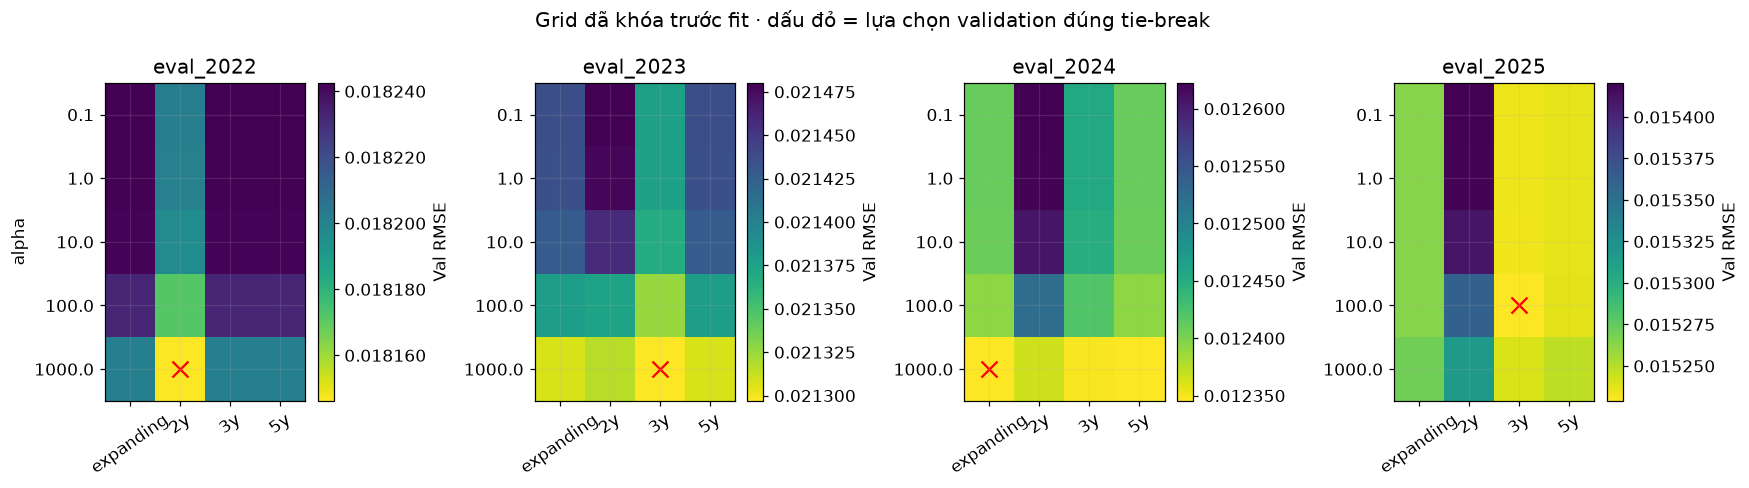
\includegraphics[width=\textwidth]{07_ridge_validation_grid.png}
        \caption{Lưới chọn lọc $\alpha$ và cửa sổ}
        \label{fig:ch4_ridge_grid}
    \end{subfigure}
    \hfill
    \begin{subfigure}[b]{0.49\textwidth}
        \centering
        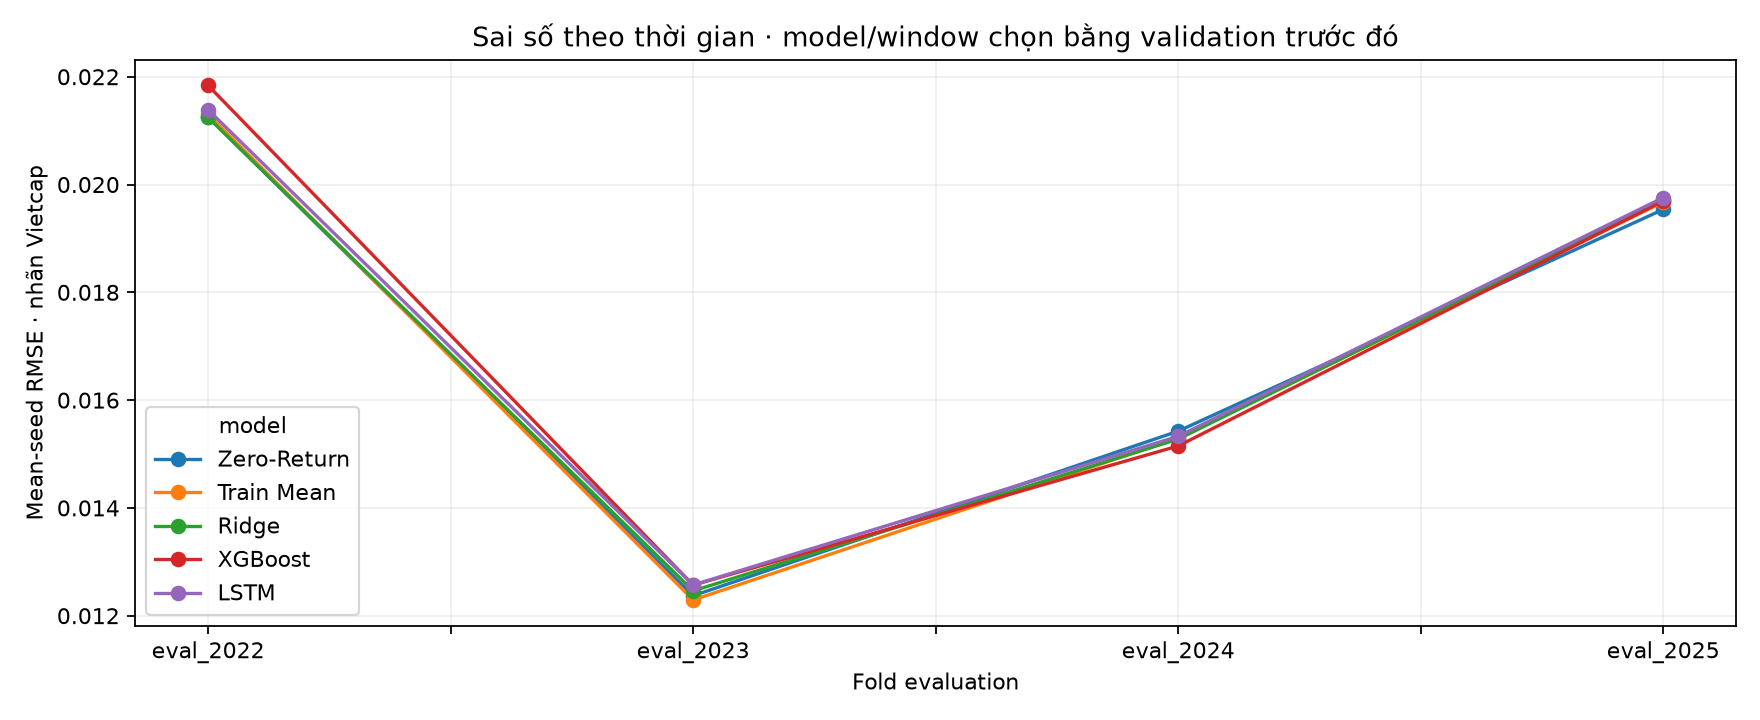
\includegraphics[width=\textwidth]{19_ridge_errors_by_year.png}
        \caption{Sai số trung bình qua từng năm}
        \label{fig:ch4_errors_year}
    \end{subfigure}
    \caption{Kết quả tinh chỉnh siêu tham số Ridge và phân bố sai số theo từng năm giai đoạn 2022--2025.}
    \label{fig:ch4_ridge_pair}
\end{figure}

\begin{figure}[H]
    \centering
    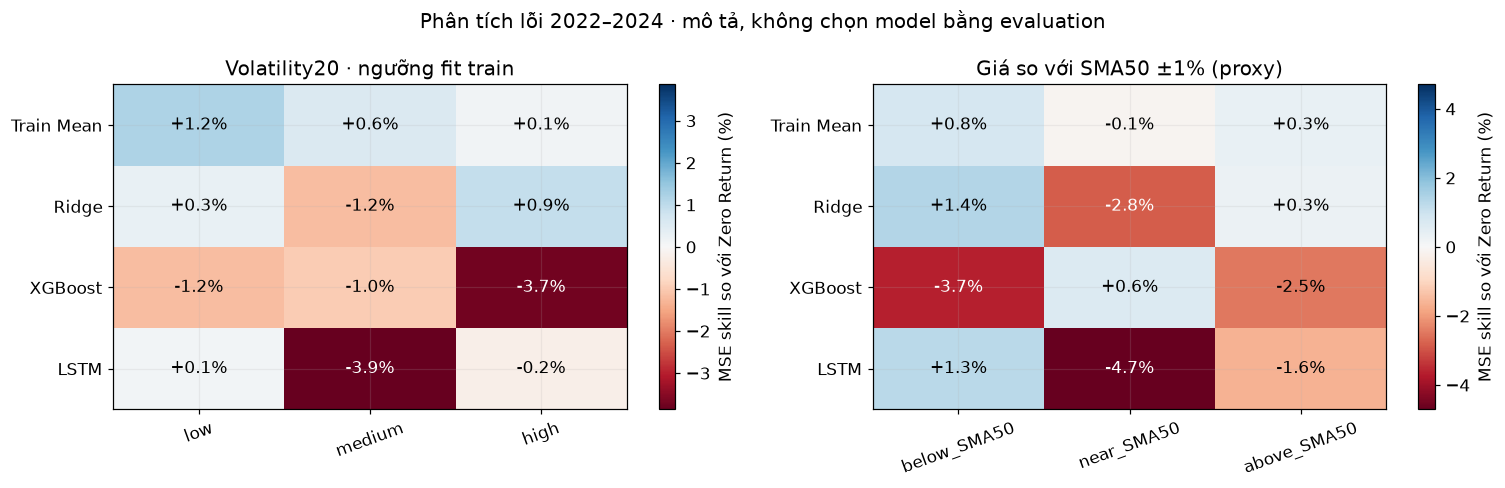
\includegraphics[width=0.90\textwidth]{15_ridge_error_regimes.png}
    \caption{Phân tích sai số mô hình Ridge theo các trạng thái biến động thị trường (Error Regimes).}
    \label{fig:ch4_error_regimes}
\end{figure}

\begin{table}[H]
\centering
\caption{Tổng hợp hiệu năng Walk-Forward của các chiến lược chọn lọc Ridge}
\label{tab:ch4_ridge_refinement}
\renewcommand{\arraystretch}{1.18}
\small
\setlength{\tabcolsep}{4.5pt}%
\resizebox{\ifdim\width>\textwidth\textwidth\else\width\fi}{!}{%
\begin{tabular}{@{}l r r r r r@{}}
\toprule
\textbf{Chiến lược} & \textbf{Mean RMSE $\downarrow$} & \textbf{Mean MAE $\downarrow$} & \textbf{Worst-fold RMSE $\downarrow$} & \textbf{Fold dương} & \textbf{Gain vs Ridge cũ (\%)} \\
\midrule
Ridge\_joint ($\alpha$ + window) & 0,016298 & 0,011439 & 0,021277 & 2/4 & $+0,176\%$ \\
Ridge\_alpha\_only & 0,016298 & 0,011439 & 0,021277 & 2/4 & $+0,176\%$ \\
Ridge\_window\_only & 0,016327 & 0,011442 & \textbf{0,021244} & 2/4 & $0,000\%$ \\
Ridge\_expanding & 0,016354 & \textbf{0,011433} & 0,021375 & 1/4 & $-0,164\%$ \\
TrainMean\_expanding & \textbf{0,016291} & 0,011453 & 0,021278 & 2/4 & $+0,218\%$ \\
Zero-Return & 0,016350 & 0,011455 & 0,021254 & 0/4 & $-0,138\%$ \\
\bottomrule
\end{tabular}%
}
\end{table}

Hình~\ref{fig:ch4_ridge_pair}, Hình~\ref{fig:ch4_error_regimes} và Bảng~\ref{tab:ch4_ridge_refinement} minh chứng rõ: chiến lược chọn lọc kết hợp (\nolinkurl{Ridge_joint}) xác định cặp siêu tham số tối ưu cho fold mới nhất là $\alpha = 100$ cùng cửa sổ $3$ năm, giúp cải thiện $0,176\%$ Mean RMSE so với chiến lược giữ nguyên cửa sổ mở rộng (\nolinkurl{Ridge_expanding}) và vượt qua đường cơ sở \nolinkurl{Zero-Return}.

\section{Kiểm định trên dữ liệu năm 2026 và Tác động của Recency + \texttt{bias60}}

\subsection{Sự suy giảm của các mô hình đóng băng trên năm 2026}
Trong vòng kiểm định \textit{Evaluation 2026} (mã \texttt{20261030T\-014012158951Z}, 0 fit mới), nhóm chấm điểm toàn bộ các mô hình đã khóa trọng số từ cuối 2023 hoặc v2 trên tập 200 cặp chung và 202 cặp Vietcap đầu năm đến 29/10/2026.

\begin{table}[H]
\centering
\caption{Hiệu năng các mô hình lịch sử đóng băng trên năm 2026 (Cohort chung $n=200$ và Vietcap $n=202$)}
\label{tab:ch4_frozen_2026}
\renewcommand{\arraystretch}{1.18}
\small
\setlength{\tabcolsep}{4.5pt}%
\resizebox{\ifdim\width>\textwidth\textwidth\else\width\fi}{!}{%
\begin{tabular}{@{}l l r r r r r r@{}}
\toprule
\textbf{Mô hình đóng băng} & \textbf{Cohort} & \textbf{n} & \textbf{RMSE $\downarrow$} & \textbf{MAE Giá (VNĐ)} & \textbf{Hit (\%)} & \textbf{Balanced (\%)} & \textbf{Skill vs Zero} \\
\midrule
Zero-Return & common & 200 & \textbf{0,020114} & \textbf{1.082,06} & N/A & N/A & 0,0000 \\
LSTM\_serving & common & 200 & 0,020428 & 1.092,46 & \textbf{51,28} & \textbf{54,27} & $-0,0315$ \\
XGBoost\_serving & common & 200 & 0,020489 & 1.106,21 & 43,59 & 47,65 & $-0,0376$ \\
Ridge\_serving & common & 200 & 0,020530 & 1.090,73 & 46,15 & 50,43 & $-0,0419$ \\
Ridge\_research\_new ($\le 2023$) & vci\_full & 202 & 0,020706 & 1.114,18 & 43,15 & 49,96 & $-0,0595$ \\
\bottomrule
\end{tabular}%
}
\end{table}

\begin{figure}[H]
    \centering
    \begin{subfigure}[b]{0.49\textwidth}
        \centering
        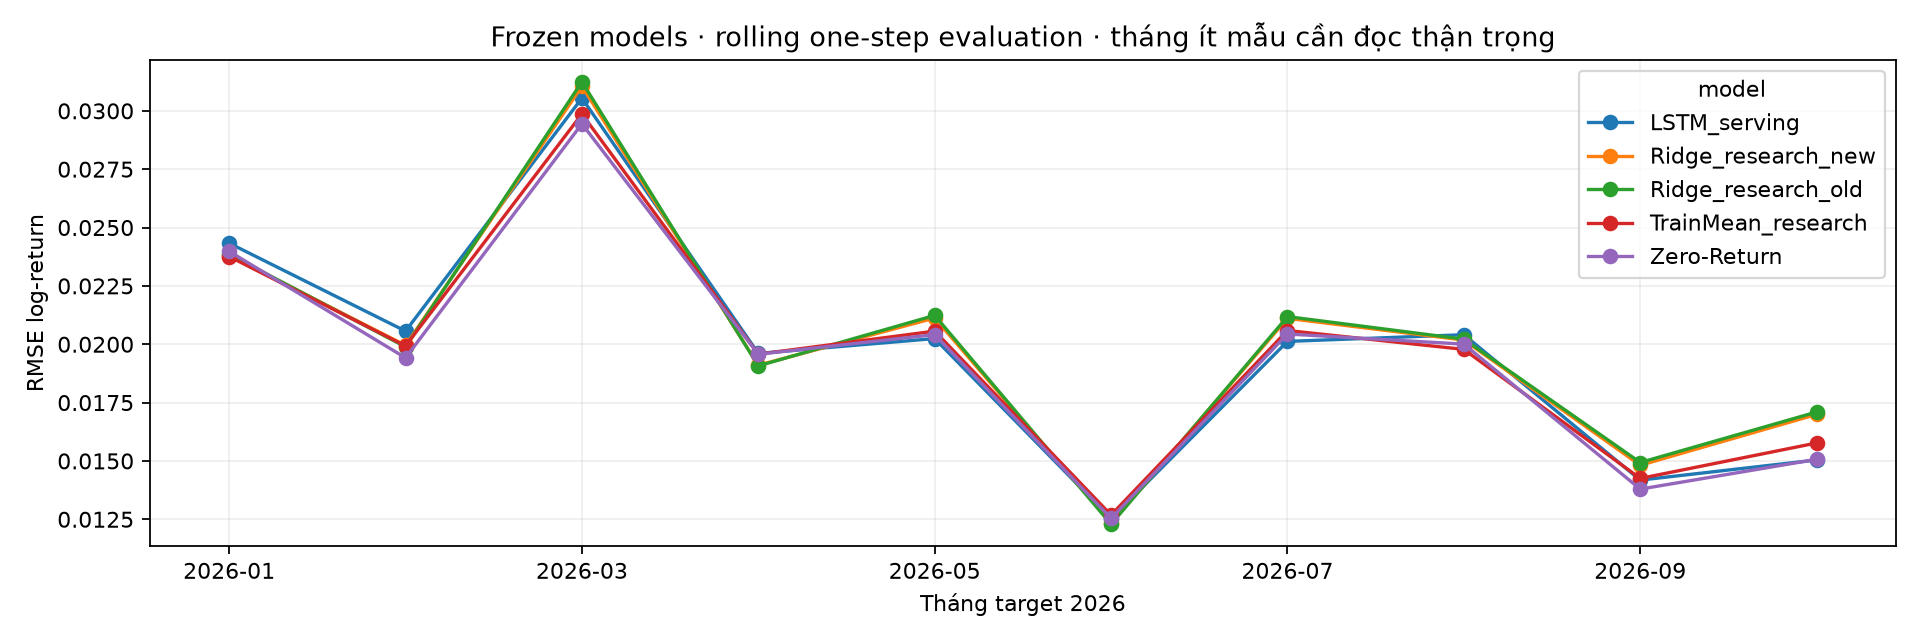
\includegraphics[width=\textwidth]{13_eval2026_monthly_errors.png}
        \caption{Sai số theo từng tháng năm 2026}
    \end{subfigure}
    \hfill
    \begin{subfigure}[b]{0.49\textwidth}
        \centering
        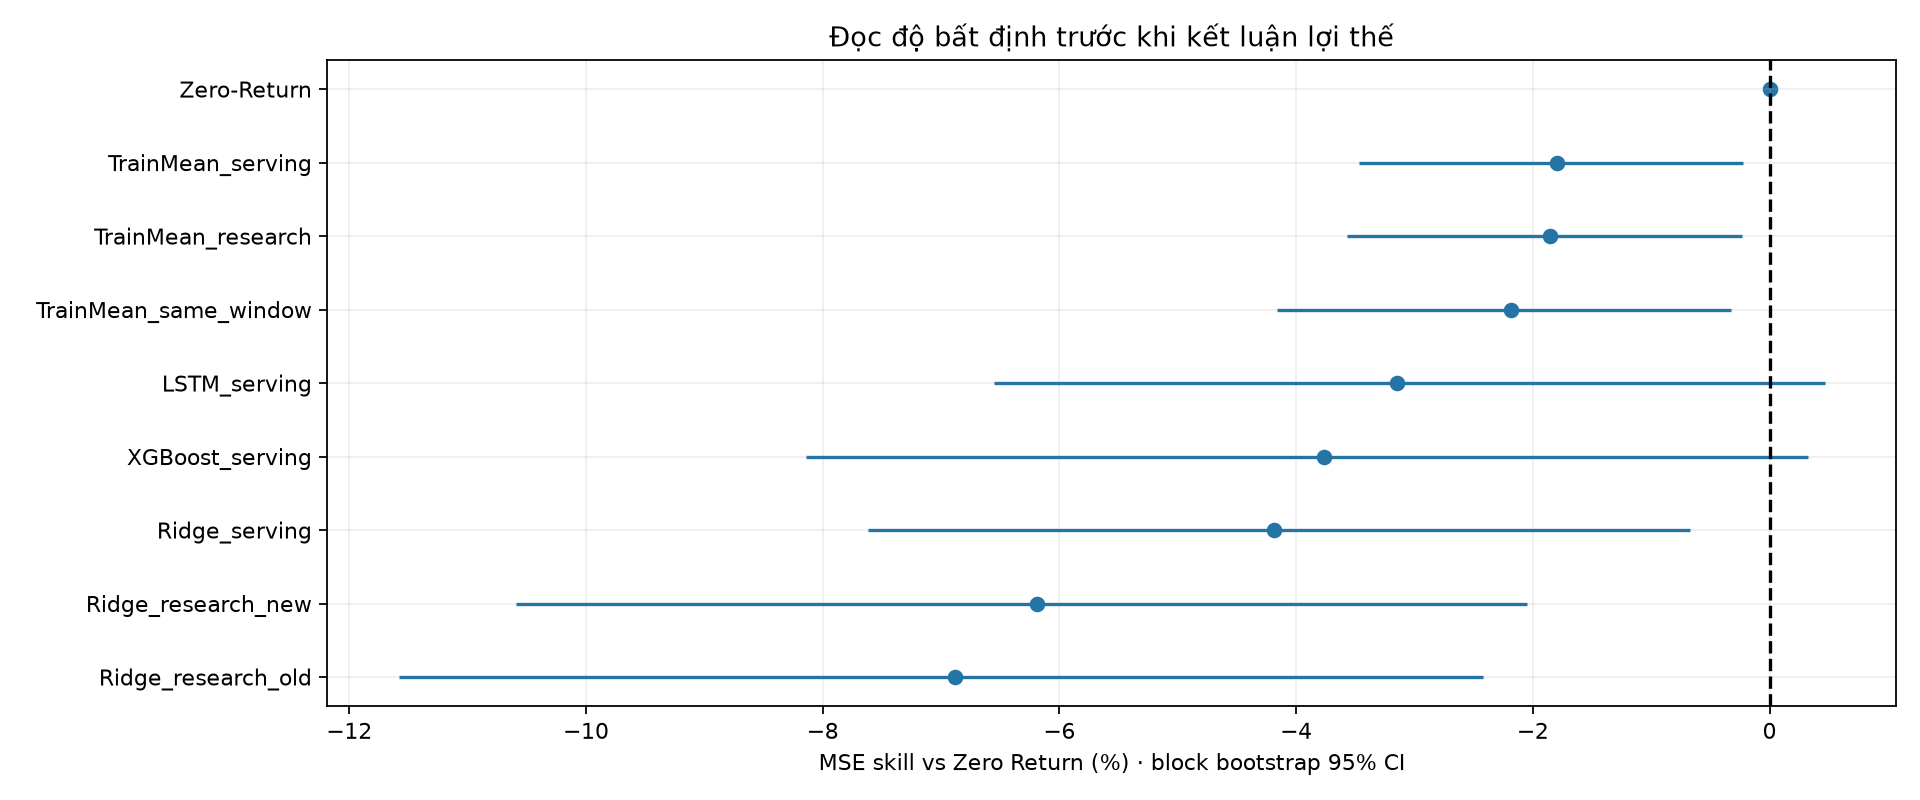
\includegraphics[width=\textwidth]{14_eval2026_skill_intervals.png}
        \caption{MSE Skill và khoảng tin cậy CI 95\%}
    \end{subfigure}
    \caption{Kết quả kiểm định mô hình đóng băng trên năm 2026: mọi mô hình cũ đều thua \nolinkurl{Zero-Return}.}
    \label{fig:ch4_eval2026_pair}
\end{figure}

Bảng~\ref{tab:ch4_frozen_2026} và Hình~\ref{fig:ch4_eval2026_pair} cho thấy các mô hình đóng băng từ giai đoạn trước đều suy giảm hiệu năng khi sang năm 2026 (MSE Skill âm từ $-3,15\%$ đến $-5,95\%$) do độ trễ dữ liệu (\textit{model staleness}) và sự đảo chiều xu hướng của cổ phiếu FPT.

\subsection{Tác động của cập nhật trọng số (Refit $\le 2025$) và hiệu chỉnh \texttt{bias60}}
Trong Đợt huấn luyện 5 (\textit{Recency \& Bias Study} mã \texttt{20261030T\-022440928507Z}), nhóm kiểm chứng trên cùng 202 phiên Vietcap năm 2026 (197 phiên có biến động khác 0) xem việc cập nhật trọng số tới hết năm 2025 kết hợp hiệu chỉnh nhân quả \texttt{bias60} có khắc phục được hiện tượng lệch pha hay không.

\begin{table}[H]
\centering
\caption{Đối chứng chiến lược Recency và \texttt{bias60} trên 202 phiên năm 2026}
\label{tab:ch4_recency_bias}
\renewcommand{\arraystretch}{1.2}
\small
\setlength{\tabcolsep}{4.5pt}%
\resizebox{\ifdim\width>\textwidth\textwidth\else\width\fi}{!}{%
\begin{tabular}{@{}l r r r r@{}}
\toprule
\textbf{Chiến lược lịch sử} & \textbf{RMSE return $\downarrow$} & \textbf{MAE giá (VNĐ) $\downarrow$} & \textbf{Hit / 197 (\%)} & \textbf{Balanced Acc (\%)} \\
\midrule
Ridge frozen (train $\le 2023$) & 0,0207058 & 1.114,18 & 43,15\% & 49,96\% \\
Ridge refit (train $\le 2025$) & 0,0201191 & 1.080,94 & 50,76\% & 54,20\% \\
\textbf{Ridge refit ($\le 2025$) + \texttt{bias60}} & \textbf{0,0201116} & \textbf{1.064,12} & \textbf{60,91\%} & \textbf{56,62\%} \\
Ridge monthly refit & 0,0201124 & 1.074,00 & 52,79\% & 54,52\% \\
Zero Return (Baseline) & 0,0201157 & 1.081,70 & N/A & N/A \\
\bottomrule
\end{tabular}%
}
\end{table}

\begin{figure}[H]
    \centering
    \begin{subfigure}[b]{0.49\textwidth}
        \centering
        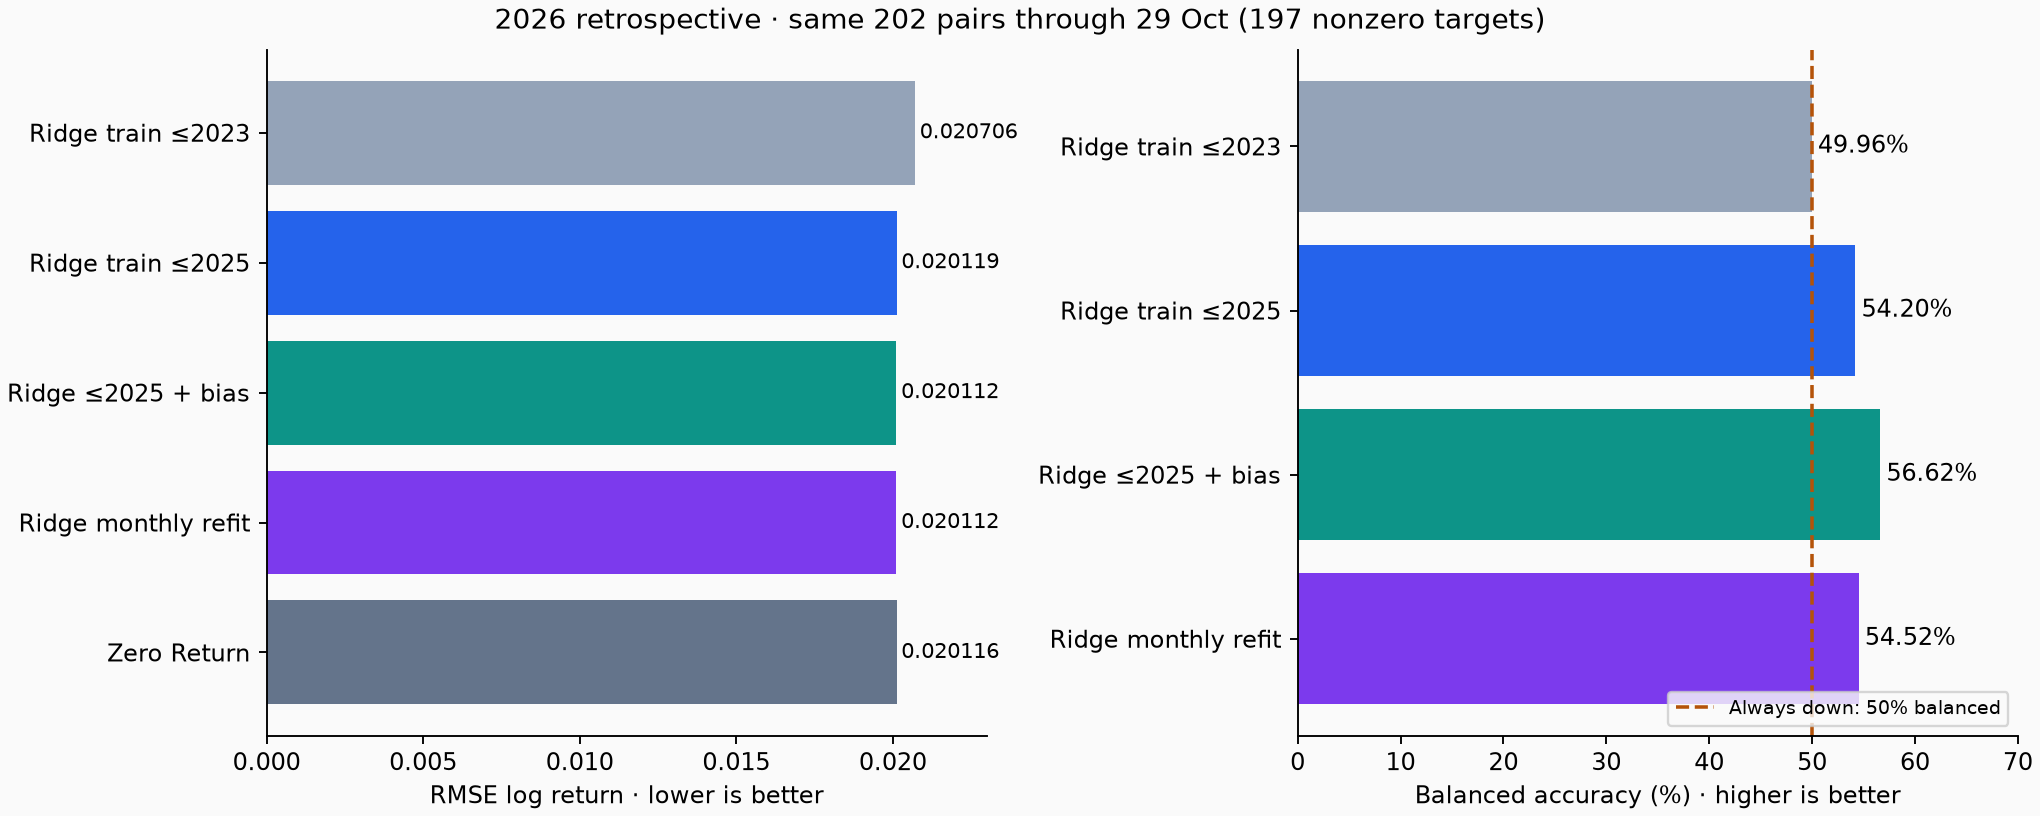
\includegraphics[width=\textwidth]{01_recency_bias.png}
        \caption{RMSE và Balanced Accuracy năm 2026}
    \end{subfigure}
    \hfill
    \begin{subfigure}[b]{0.49\textwidth}
        \centering
        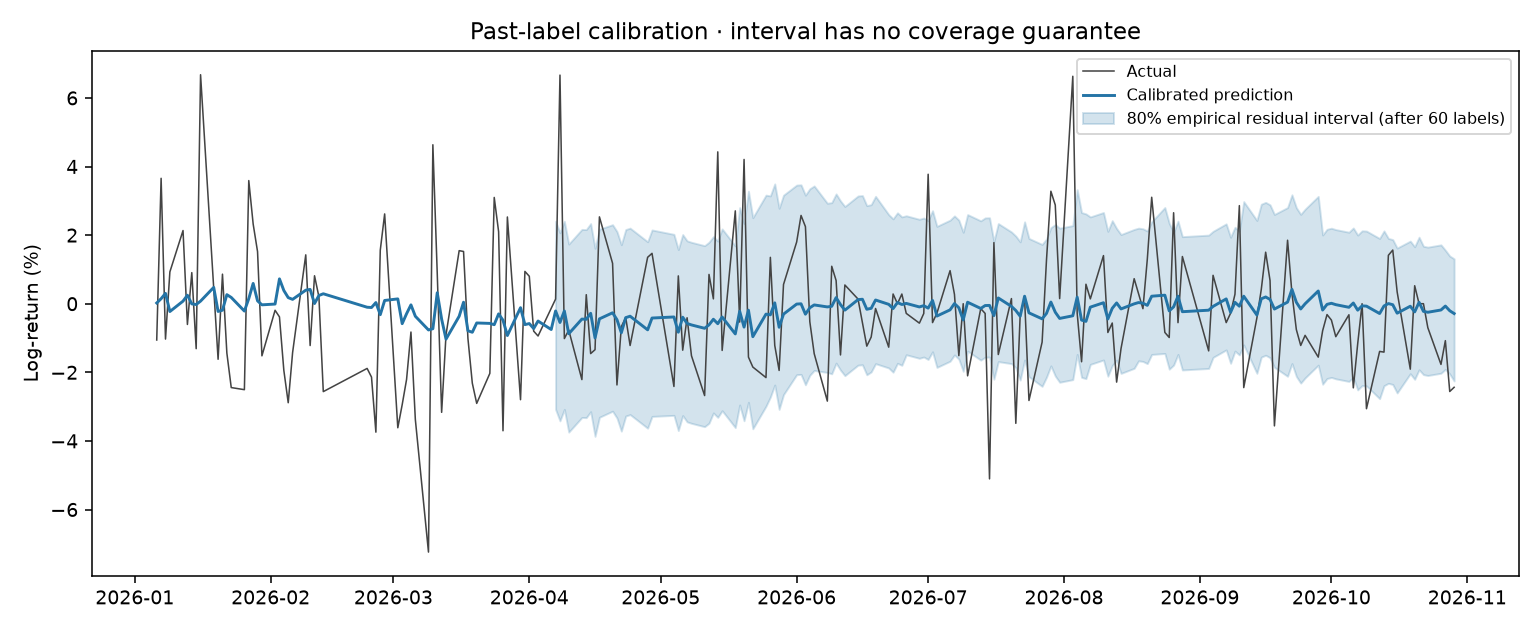
\includegraphics[width=\textwidth]{16_empirical_interval.png}
        \caption{Độ phủ khoảng sai số thực nghiệm}
    \end{subfigure}
    \caption{So sánh hiệu năng cập nhật dữ liệu mới (Refit) và hiệu chỉnh nhân quả \texttt{bias60} trên 202 phiên năm 2026.}
    \label{fig:ch4_recency_pair}
\end{figure}

Từ Bảng~\ref{tab:ch4_recency_bias} và Hình~\ref{fig:ch4_recency_pair}, có hai kết quả chính:
\begin{itemize}
    \item Huấn luyện lại trên 3 năm gần nhất đến cuối 2025 giúp giảm ngay \textbf{2,83\% RMSE} so với bản đóng băng 2023 ($0,0207058 \to 0,0201191$), đưa Balanced Accuracy từ $49,96\%$ lên $54,20\%$.
    \item Cộng thêm hiệu chỉnh nhân quả \textbf{\texttt{bias60}} giúp giảm tiếp RMSE về \textbf{$0,0201116$} (thấp hơn \texttt{Zero Return} $0,0201157$), đạt \textbf{MAE giá thấp nhất bảng (1.064,12 VNĐ)}, Hit Rate \textbf{60,91\%} và Balanced Accuracy \textbf{56,62\%}. Tuy nhiên, mức cải thiện MSE Skill so với Zero Return chỉ khoảng $+0,041\%$ với CI 95\% vẫn chứa 0, cho thấy lợi thế về độ lớn sai số còn nhỏ dù phân biệt xu hướng đã cải thiện rõ.
\end{itemize}

\section{Đối chứng trực tiếp giữa \texttt{Ridge+bias60} và \texttt{LSTM} (104 phiên 06--10/2026)}
Trong nghiên cứu \textit{Period Comparison} (\texttt{20261030T\-024048531444Z}), nhóm đặt \textbf{\texttt{Ridge+bias60}} đối chứng trực tiếp trên cùng \textbf{104 phiên giao dịch từ ngày 01/06/2026 đến ngày 29/10/2026} (99 phiên biến động khác 0) cùng với \textbf{\texttt{LSTM (lookback 30)}} và \textbf{\texttt{Zero Return}}.

\begin{figure}[H]
    \centering
    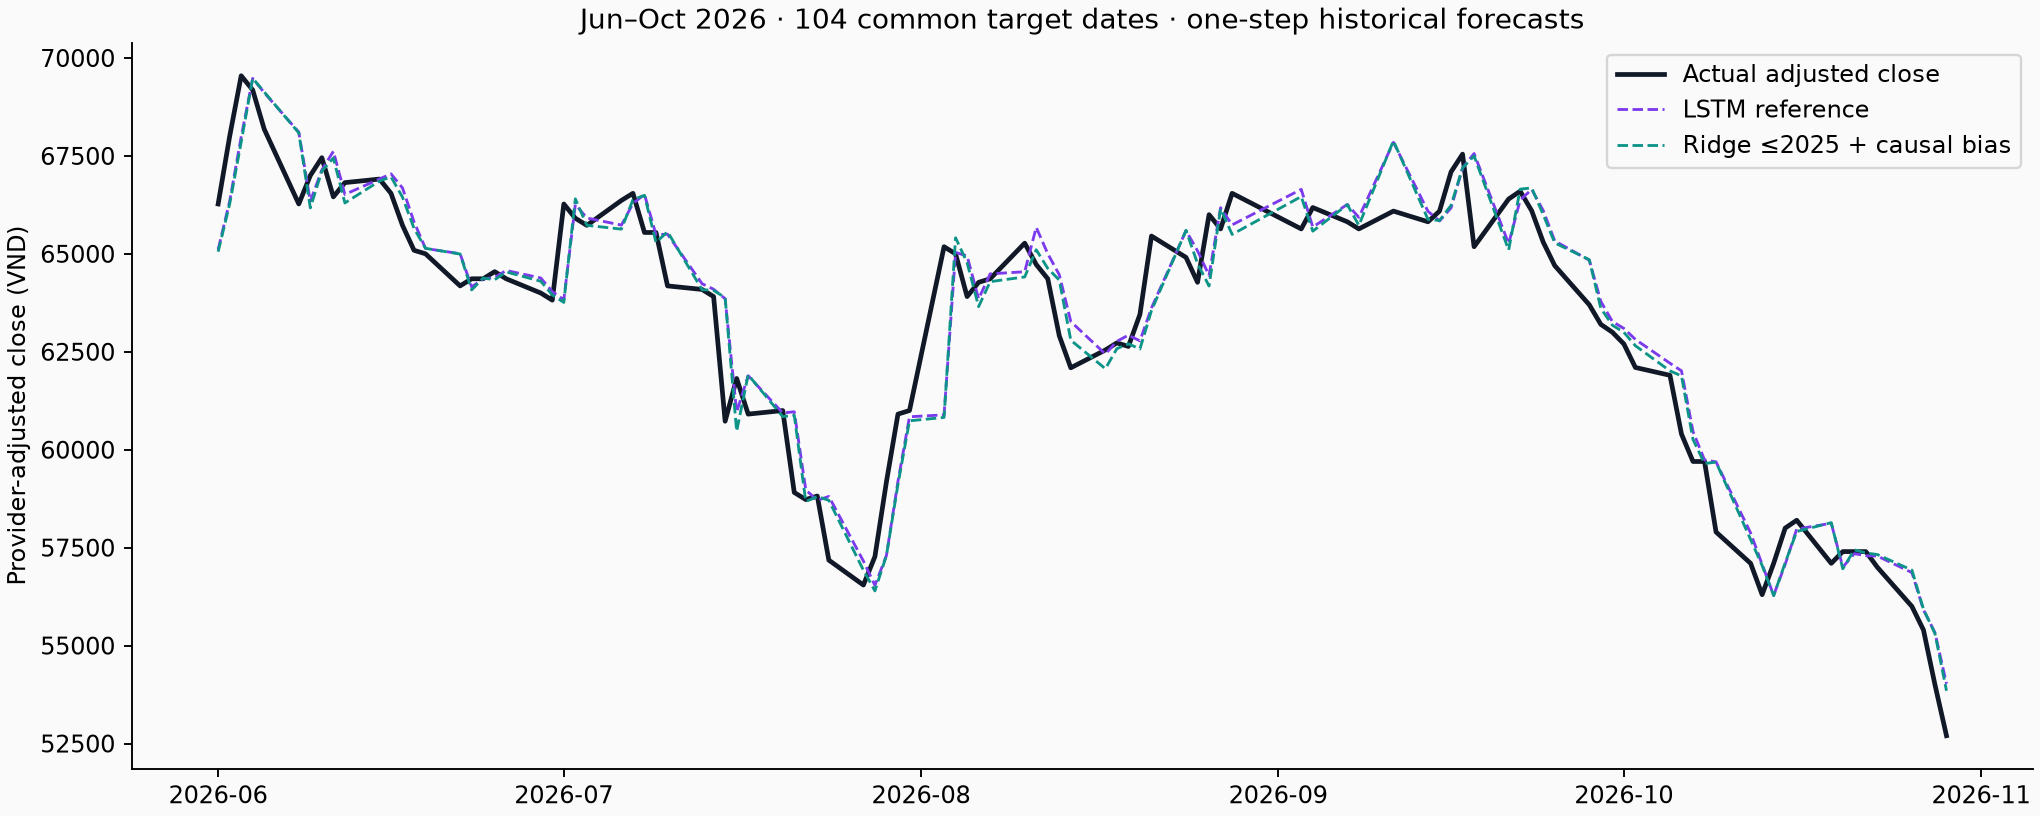
\includegraphics[width=0.95\textwidth]{03_actual_predictions.png}
    \caption{Chuỗi giá thực tế và dự báo một bước ($h=1$) của \texttt{Ridge+bias60}, \texttt{LSTM} và \texttt{Zero Return} trên 104 phiên (01/06 -- 29/10/2026).}
    \label{fig:ch4_actual_104}
\end{figure}

\begin{figure}[H]
    \centering
    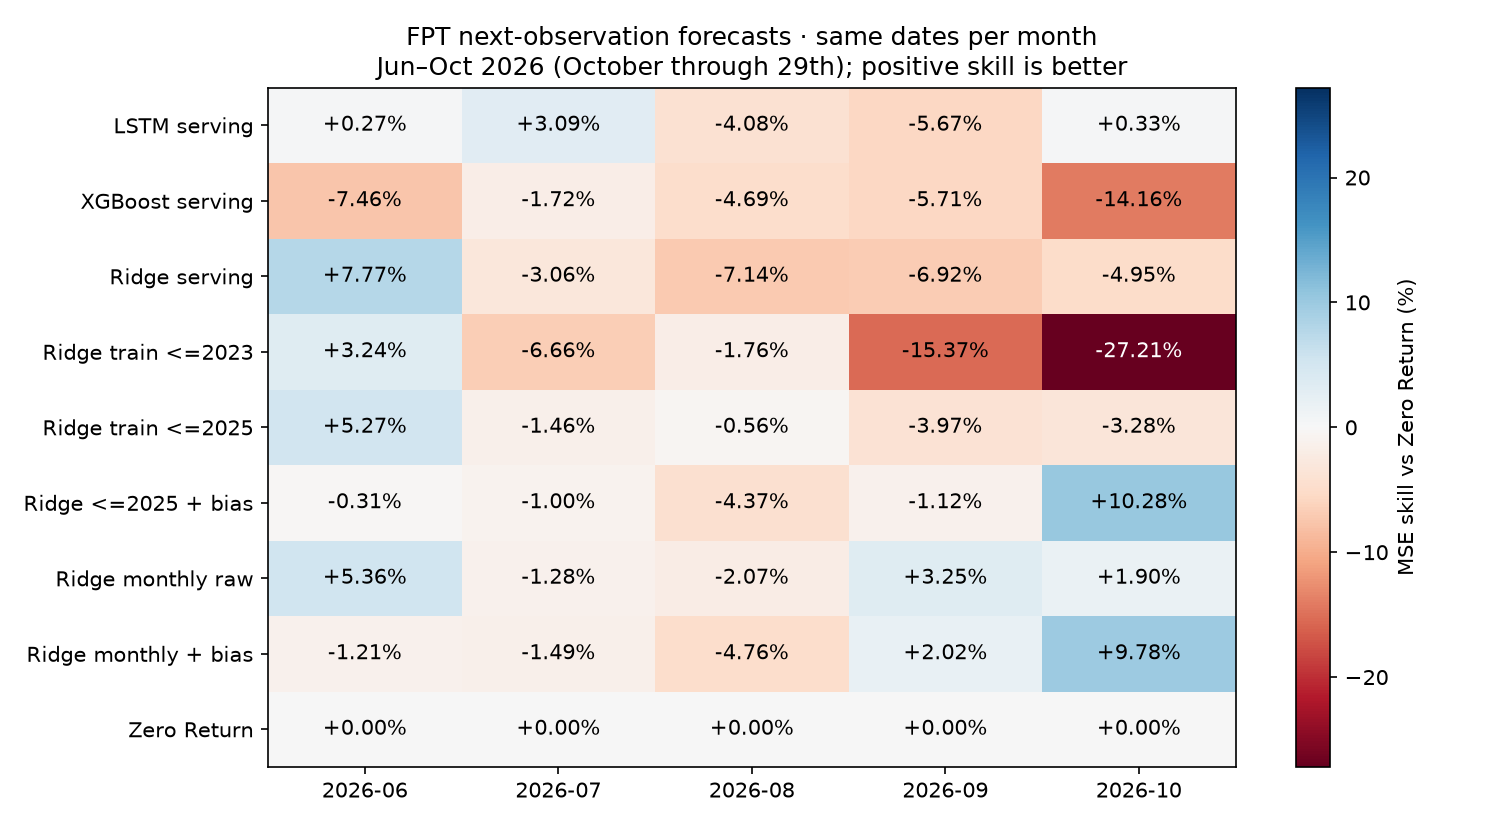
\includegraphics[width=0.90\textwidth]{20_period_monthly_skill.png}
    \caption{Phân rã MSE Skill và độ chính xác theo từng tháng (tháng 6 đến tháng 10/2026) giữa các mô hình.}
    \label{fig:ch4_monthly_skill}
\end{figure}

\begin{table}[H]
\centering
\caption{Bảng đối chứng chi tiết trên 104 phiên chung từ 01/06 đến 29/10/2026}
\label{tab:ch4_period_104}
\renewcommand{\arraystretch}{1.18}
\small
\setlength{\tabcolsep}{4.5pt}%
\resizebox{\ifdim\width>\textwidth\textwidth\else\width\fi}{!}{%
\begin{tabular}{@{}l r r r r r r@{}}
\toprule
\textbf{Mô hình / Chiến lược} & \textbf{RMSE $\downarrow$} & \textbf{MAE Giá (VNĐ) $\downarrow$} & \textbf{Hit (\%)} & \textbf{Balanced (\%)} & \textbf{Sai số $\le 1\%$} & \textbf{Sai số $\le 2\%$} \\
\midrule
Zero-Return (Baseline) & \textbf{0,016775} & 771,84 & N/A & N/A & -- & -- \\
\textbf{Ridge\_refit2025 + \texttt{bias60}} & 0,016776 & \textbf{767,28} & \textbf{62,63\%} & \textbf{57,95\%} & \textbf{53,85\%} & 79,81\% \\
Ridge\_monthly\_refit & 0,016746 & 771,17 & 55,56\% & 57,05\% & 49,04\% & \textbf{80,77\%} \\
Ridge\_refit2025 (raw) & 0,016859 & 781,62 & 50,51\% & 55,13\% & 50,00\% & 80,77\% \\
LSTM\_serving (lb=30) & 0,016831 & 786,38 & 47,47\% & 50,83\% & 50,00\% & 80,77\% \\
Ridge\_frozen\_2023 & 0,017465 & 814,51 & 41,41\% & 49,87\% & 49,04\% & 78,85\% \\
\bottomrule
\end{tabular}%
}
\end{table}

Bảng~\ref{tab:ch4_period_104} cùng Hình~\ref{fig:ch4_actual_104} và Hình~\ref{fig:ch4_monthly_skill} cho thấy sự khác biệt rõ rệt giữa hai mô hình:
\begin{itemize}
    \item Trên cùng 104 phiên giao dịch thực tế, mô hình học sâu \nolinkurl{LSTM_serving} bị lệch pha dự báo tăng quá mức (Recall tăng $66,67\%$, Recall giảm chỉ $35,00\%$), khiến Hit Rate rơi xuống \textbf{47,47\%} và Balanced Accuracy chỉ đạt \textbf{50,83\%}, MAE giá là $786,38$ VNĐ.
    \item Trái lại, \texttt{Ridge ($\le 2025$) + bias60} đạt sai số MAE giá thấp nhất (\textbf{767,28 VNĐ}), tỷ lệ ngày có sai lệch giá trong phạm vi $\le 1\%$ cao nhất (\textbf{53,85\%}), Hit Rate \textbf{62,63\%} và Balanced Accuracy \textbf{57,95\%}. Đồng thời, biểu đồ theo từng tháng (Hình~\ref{fig:ch4_monthly_skill}) cũng cho thấy mô hình chỉ tốt hơn ở một số tháng nhất định và vẫn kém baseline trong các tháng thị trường biến động bất ngờ.
\end{itemize}

\section{Kiểm định dự báo đa bước ($h=5, 21, 22$) và Nâng cấp \texttt{v1} $\to$ \texttt{v4}}
Sau khi đưa vào vận hành tính năng mô phỏng nhiều bước trên giao diện, nhóm tiến hành rà soát và kiểm định hồi cứu chặt chẽ trên 121--122 ngày gốc năm 2026 (từ 06/04 đến 30/09/2026):
\begin{enumerate}
    \item \textbf{Loại bỏ trôi dạt đệ quy (\texttt{v1} $\to$ \texttt{v2}):} Phát hiện phiên bản \texttt{v1} cộng \texttt{bias60} ($-0,352\%$/ngày) vào mọi bước đệ quy khiến dự báo 1 tháng sụt giảm giả tạo $-8,69\%$. Khi chuyển sang \texttt{v2} (chỉ dùng bias cho bước 1 đã kiểm chứng, từ bước 2 chạy Ridge thô), kịch bản 1 tháng tại gốc 29/10 ($52.700$ VNĐ) trở về mức hợp lý \textbf{51.659,71 VNĐ ($-1,974\%$)}.
    \item \textbf{Căn tâm nhiễu Bootstrap (\texttt{v2} $\to$ \texttt{v3}):} Trừ trung bình pool $-0,002926$ trước khi lấy mẫu khối 5 phiên giúp tách biệt vị trí đường điểm khỏi độ lệch của phân phối nhiễu. Kết quả trên 122 ngày gốc (Bảng~\ref{tab:ch4_bootstrap_v2v3} và Hình~\ref{fig:ch4_recursive_boot}) cho thấy độ phủ (Coverage) của \texttt{Ridge+bias60} ở kỳ hạn $h=5$ tăng mạnh từ \textbf{$74,59\%$ lên $82,79\%$} (sát chuẩn danh nghĩa $80\%$), ở $h=21$ tăng từ $63,11\%$ lên $77,05\%$, và điểm phạt Interval Score giảm mạnh từ $0,43387$ xuống $0,31582$.
    \item \textbf{Thử nghiệm hiệu chỉnh độ rộng biên độ (\texttt{v4}):} Thử nghiệm 121 ngày gốc chạy chính hàm \texttt{forecast()} tại $h=5$ và $h=22$ với phép nới log-distance band $L' = p + s(L-p)$, $U' = p + s(U-p)$ theo quy tắc hiệu chỉnh phân tách (\textit{Split Calibration} \cite{lei2018conformal}, Hình~\ref{fig:ch4_recursive_all} và Hình~\ref{fig:ch4_horizon_cal}). Tuy nhiên, trên tập kiểm định đến sau (62 ngày gốc từ 01/07--29/09), hệ số nới trượt $s > 1$ làm tăng nhẹ Interval Score tại $h=5$ ($0,17170 \to 0,17880$) nên không vượt qua cổng kiểm duyệt chất lượng. Hệ thống bảo toàn hệ số hoạt động \textbf{$1\times$} và hiển thị cảnh báo rõ ràng trên UI.
\end{enumerate}

\begin{table}[H]
\centering
\caption{Đối chứng độ phủ và điểm phạt Interval Score 80\% trước và sau khi căn tâm Bootstrap (\texttt{v2} $\to$ \texttt{v3}, 122 ngày gốc)}
\label{tab:ch4_bootstrap_v2v3}
\renewcommand{\arraystretch}{1.18}
\small
\setlength{\tabcolsep}{4.5pt}%
\resizebox{\ifdim\width>\textwidth\textwidth\else\width\fi}{!}{%
\begin{tabular}{@{}l r r r r@{}}
\toprule
\textbf{Mô hình} & \textbf{Kỳ hạn $h$} & \textbf{Coverage \texttt{v2} $\to$ \texttt{v3}} & \textbf{Độ rộng log TB} & \textbf{Interval Score \texttt{v2} $\to$ \texttt{v3} $\downarrow$} \\
\midrule
Ridge (raw) & 5 & 81,15\% $\to$ 78,69\% & 0,10588 & 0,15430 $\to$ 0,14731 \\
\textbf{Ridge+bias60} & 5 & \textbf{74,59\% $\to$ 82,79\%} & 0,10691 & \textbf{0,15995 $\to$ 0,14570} \\
Ridge (raw) & 21 & 70,49\% $\to$ 77,05\% & 0,21821 & 0,34933 $\to$ 0,31185 \\
\textbf{Ridge+bias60} & 21 & \textbf{63,11\% $\to$ 77,05\%} & 0,22559 & \textbf{0,43387 $\to$ 0,31582} \\
\bottomrule
\end{tabular}%
}
\end{table}

\begin{figure}[H]
    \centering
    \begin{subfigure}[b]{0.49\textwidth}
        \centering
        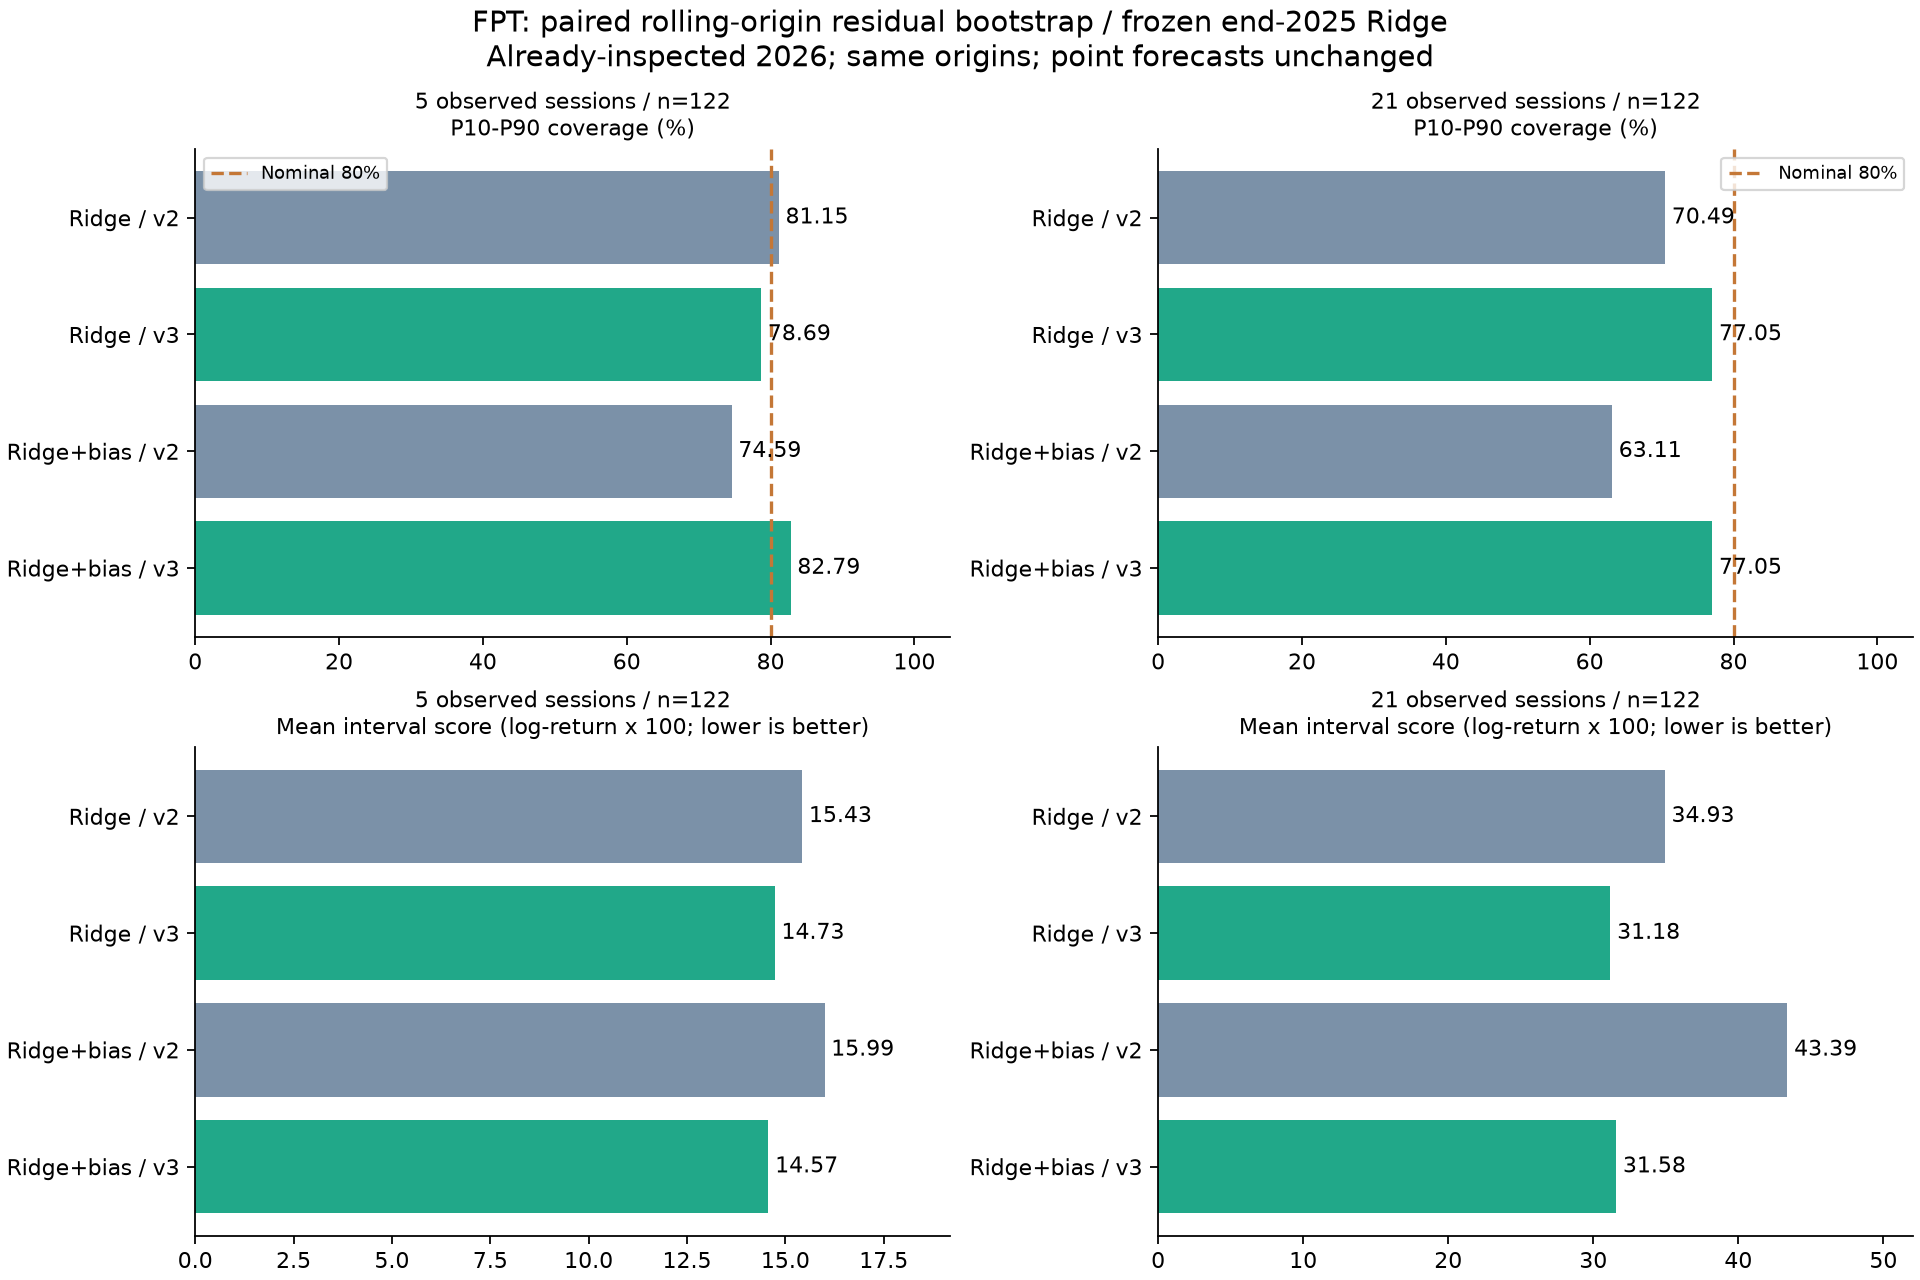
\includegraphics[width=\textwidth]{08_recursive_bootstrap.png}
        \caption{Cải thiện Coverage và Interval Score \texttt{v2} $\to$ \texttt{v3}}
        \label{fig:ch4_recursive_boot}
    \end{subfigure}
    \hfill
    \begin{subfigure}[b]{0.49\textwidth}
        \centering
        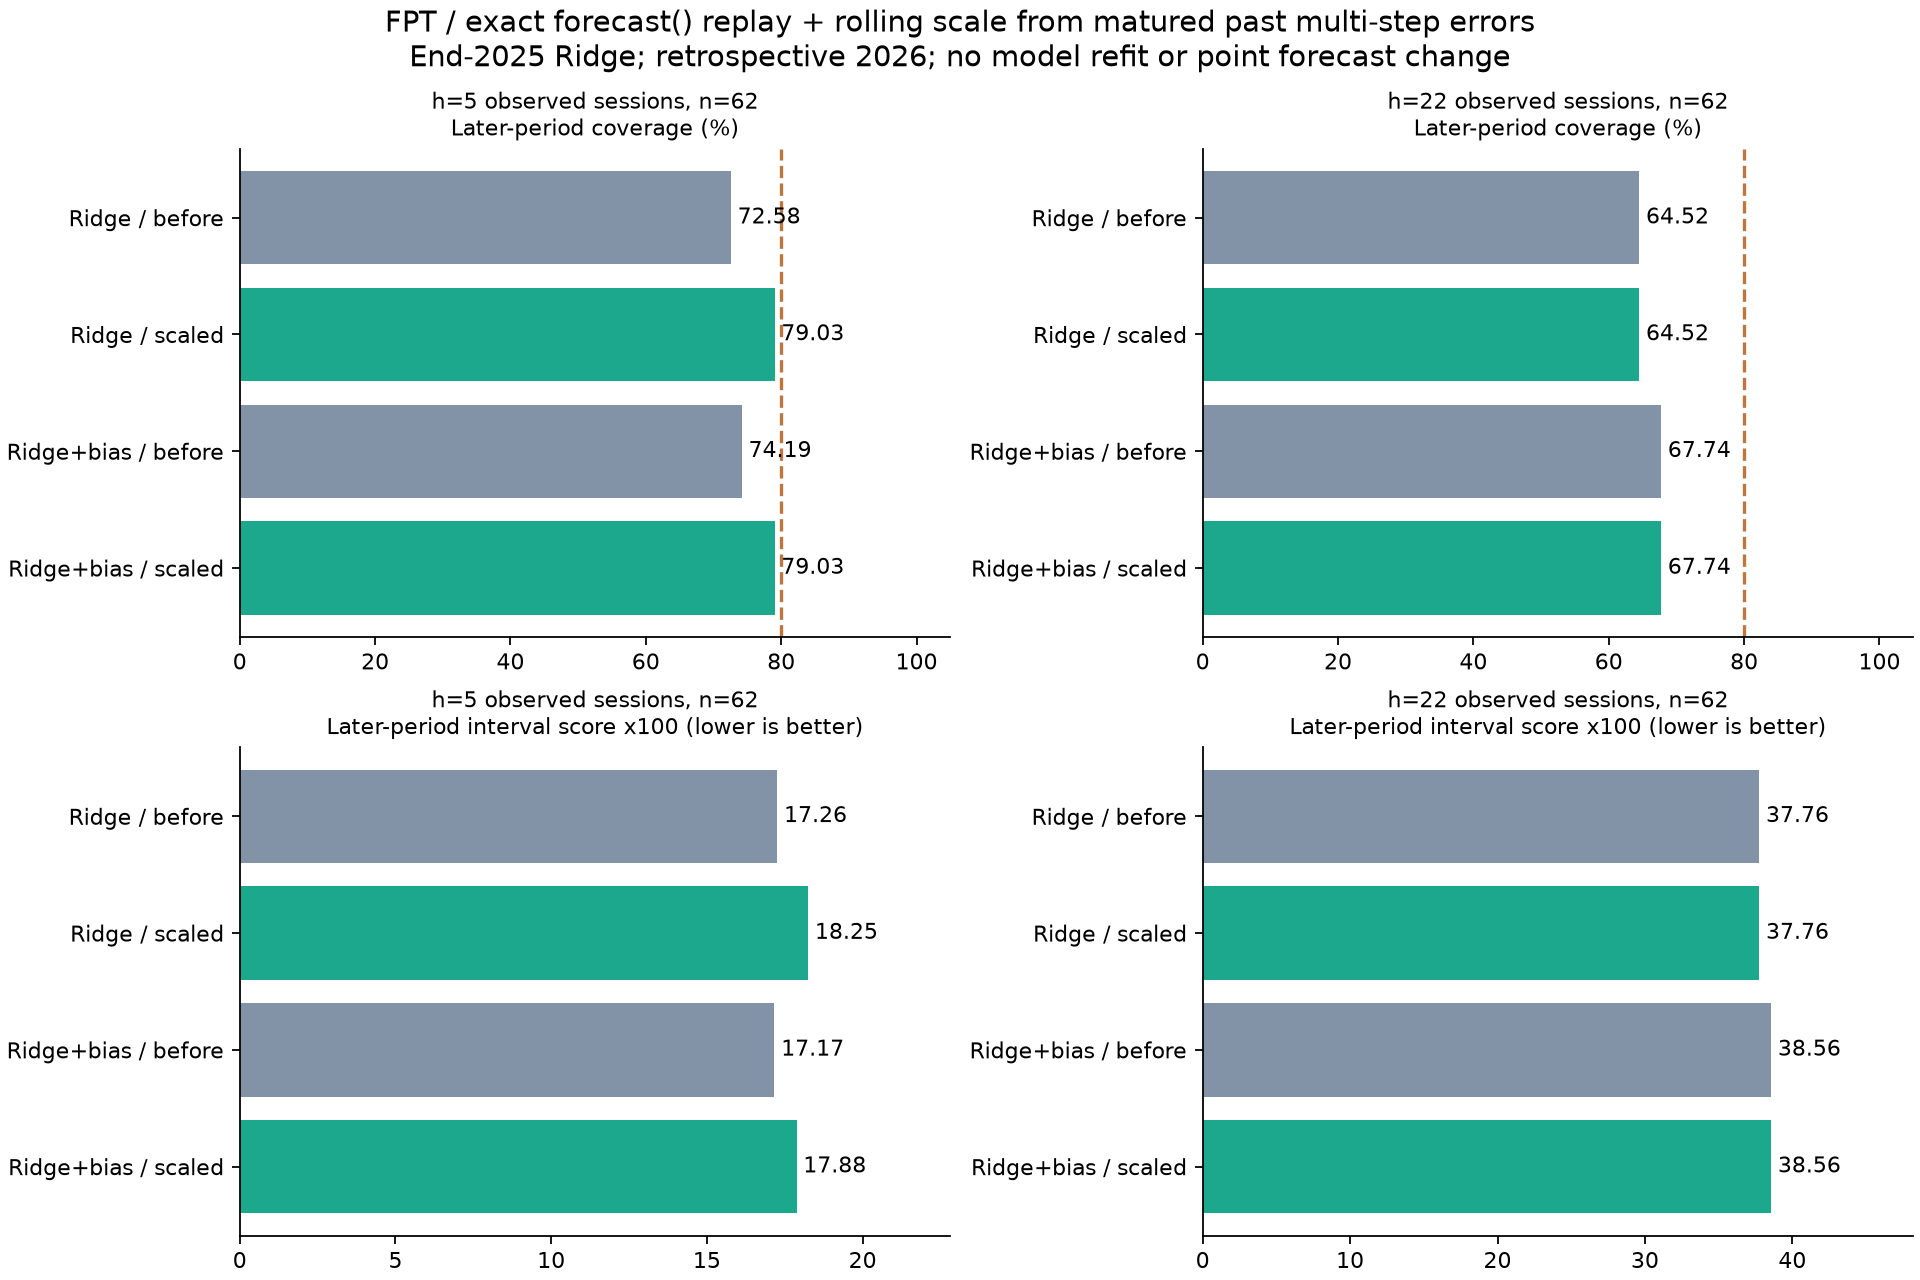
\includegraphics[width=\textwidth]{17_horizon_calibration.png}
        \caption{Thử nghiệm rolling calibration $h=5, 22$ (\texttt{v4})}
        \label{fig:ch4_horizon_cal}
    \end{subfigure}
    \caption{Kết quả kiểm định dự báo đệ quy đa bước và hiệu chỉnh vùng bất định P10--P90.}
    \label{fig:ch4_recursive_all}
\end{figure}

\section{Đối chứng cửa sổ huấn luyện cuối cùng (3 năm vs 5 năm vs Toàn bộ 2018)}
Tại Đợt huấn luyện 8 (\textit{Final Window Comparison} mã \texttt{20261101T\-014607720130Z}), nhóm chạy vòng đối chứng cuối cùng trên 16 lượt fit độc lập (18 điều kiện) nhằm khóa dứt khoát độ dài lịch sử tối ưu cho mô hình chính \texttt{Ridge6 ($\alpha = 100$)}.

\begin{table}[H]
\centering
\caption{Kết quả Walk-Forward 4 năm (2022--2025, $n=993$) giữa ba cửa sổ huấn luyện (RMSE log-return $\downarrow$)}
\label{tab:ch4_final_window}
\renewcommand{\arraystretch}{1.18}
\setlength{\tabcolsep}{4.5pt}%
\resizebox{\ifdim\width>\textwidth\textwidth\else\width\fi}{!}{%
\begin{tabular}{@{}l r r r@{}}
\toprule
\textbf{Năm đánh giá} & \textbf{Cửa sổ 3 năm} & \textbf{Cửa sổ 5 năm} & \textbf{Toàn bộ từ 2018} \\
\midrule
Năm 2022 ($n=248$) & \textbf{0,021045} & 0,021112 & 0,021112 \\
Năm 2023 ($n=248$) & 0,012397 & \textbf{0,012371} & \textbf{0,012371} \\
Năm 2024 ($n=249$) & \textbf{0,015216} & 0,015220 & 0,015269 \\
Năm 2025 ($n=248$) & \textbf{0,019655} & 0,019678 & 0,019680 \\
\midrule
\textbf{Trung bình 4 năm (Mean RMSE)} & \textbf{0,0170781} & 0,0170951 & 0,0171079 \\
\textbf{Năm tệ nhất (Worst-fold RMSE)} & \textbf{0,0210446} & 0,0211120 & 0,0211120 \\
\bottomrule
\end{tabular}%
}
\end{table}

\begin{figure}[H]
    \centering
    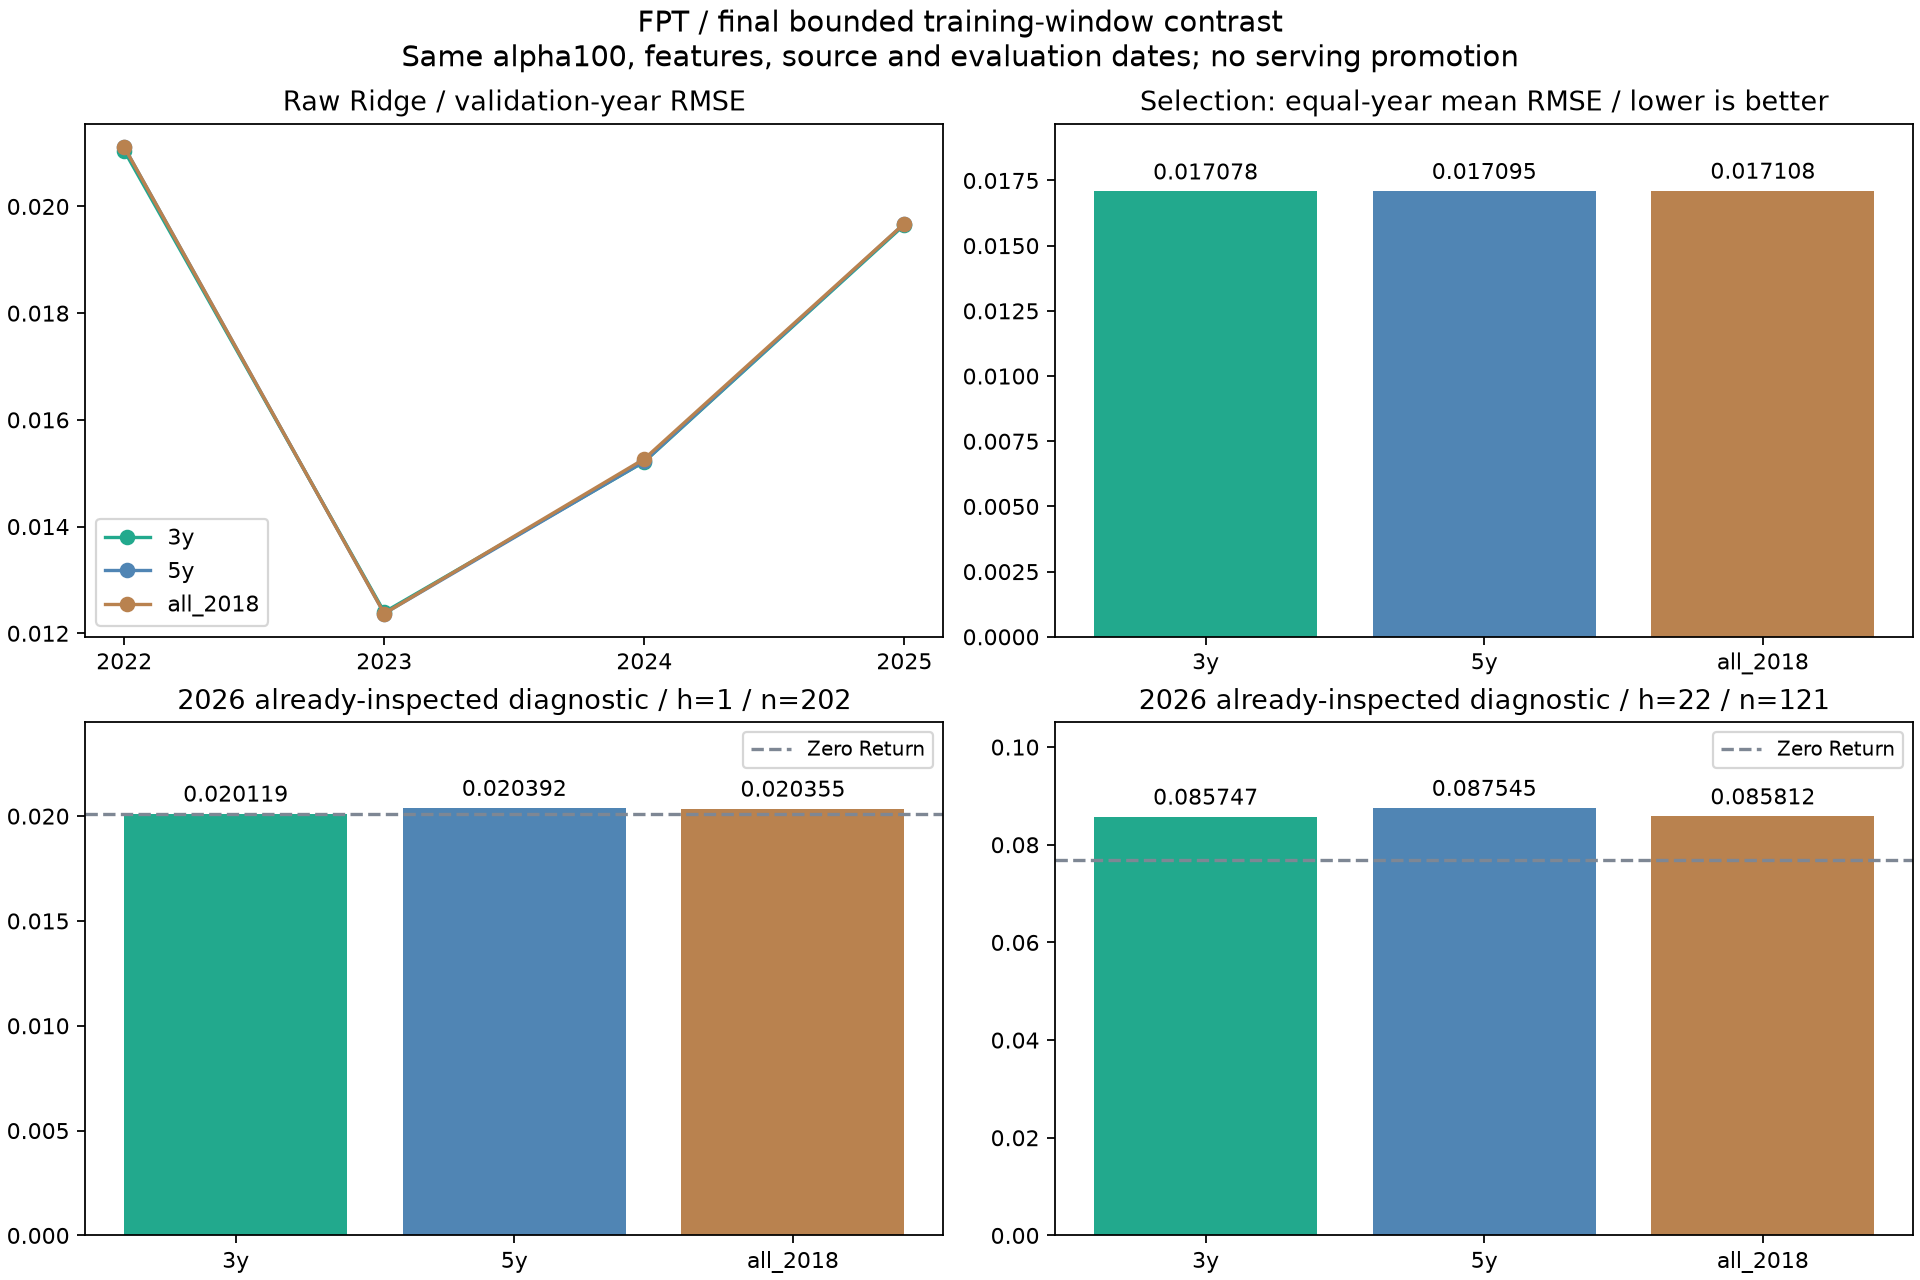
\includegraphics[width=0.92\textwidth]{09_final_window_comparison.png}
    \caption{Đối chứng cuối cùng giữa ba cửa sổ huấn luyện (3 năm, 5 năm, toàn bộ từ 2018) trên Walk-Forward 2022--2025 và chẩn đoán năm 2026.}
    \label{fig:ch4_final_window}
\end{figure}

Bảng~\ref{tab:ch4_final_window} và Hình~\ref{fig:ch4_final_window} cho thấy cửa sổ \textbf{3 năm} thắng ở \textbf{3/4 năm} (2022, 2024, 2025), có Mean RMSE thấp nhất ($0,0170781$) và sai số ở năm xấu nhất thấp nhất ($0,0210446$). Chẩn đoán trên 202 phiên năm 2026 cũng xác nhận cửa sổ \textbf{3 năm} ($n_{\text{train}} = 747$) + \texttt{bias60} đạt Hit Rate $60,91\%$ và Balanced Accuracy $56,62\%$, vượt xa cửa sổ 5 năm ($50,25\% / 46,26\%$) và toàn bộ lịch sử ($52,79\% / 48,60\%$). Khi huấn luyện lại ứng viên 3 năm tới ngày 29/10/2026 ($n_{\text{train}} = 746$), mã băm SHA-256 của mô hình trùng khớp 100\% với bundle đang phục vụ trên API.

\section{Giải phẫu trọng số mô hình phục vụ và 5 lý do chọn \texttt{Ridge6+bias60}}
Nhóm trích xuất trực tiếp tham số chuẩn hóa \texttt{StandardScaler} và bộ trọng số của tệp \nolinkurl{models/local_demo/ridge6_20261029/ridge.pkl} (Bảng~\ref{tab:ch4_ridge_weights}) để minh họa khả năng giải thích tường minh của mô hình chính:

\begin{table}[H]
\centering
\caption{Tham số chuẩn hóa và trọng số thực tế của mô hình \texttt{Ridge6 ($\alpha = 100$)} đang phục vụ}
\label{tab:ch4_ridge_weights}
\renewcommand{\arraystretch}{1.18}
\setlength{\tabcolsep}{4.5pt}%
\resizebox{\ifdim\width>\textwidth\textwidth\else\width\fi}{!}{%
\begin{tabular}{@{}l r r r p{5.5cm}@{}}
\toprule
\textbf{Đặc trưng} & \textbf{Mean ($\mu_{\text{train}}$)} & \textbf{Std ($\sigma_{\text{train}}$)} & \textbf{Trọng số ($w_j$)} & \textbf{Diễn giải hành vi thị trường} \\
\midrule
\nolinkurl{Log_Return} & $-0,000075$ & $0,018150$ & $+0,000525$ & Quán tính rất nhẹ của phiên vừa đóng cửa. \\
\nolinkurl{Return_Lag_1} & $-0,000037$ & $0,018126$ & $-0,001398$ & Hiệu ứng điều chỉnh hồi về trung bình sau T-1. \\
\nolinkurl{Return_Lag_2} & $-0,000085$ & $0,018201$ & $-0,000644$ & Áp lực chốt lời ngắn hạn trễ 2 phiên. \\
\nolinkurl{Return_Lag_5} & $-0,000081$ & $0,018213$ & $-0,001272$ & Chu kỳ điều chỉnh theo tuần (5 phiên trước). \\
\texttt{Return\_5} & $-0,000327$ & $0,040137$ & $+0,000074$ & Đóng góp trung tính của xu hướng 1 tuần. \\
\texttt{Return\_20} & $-0,001296$ & $0,083439$ & $+0,001082$ & Động lượng xu hướng trung hạn 1 tháng. \\
\midrule
\multicolumn{3}{l}{\textbf{Hệ số chặn (\texttt{Intercept} $b$):}} & \multicolumn{2}{l}{$-0,000076$ (xấp xỉ trung bình lợi suất tập Train)} \\
\multicolumn{3}{l}{\textbf{Hiệu chỉnh \texttt{bias60} đóng băng tại 29/10/2026:}} & \multicolumn{2}{l}{$-0,003521$ ($-0,352\%$/ngày trên 60 sai số gần nhất)} \\
\multicolumn{3}{l}{\textbf{Mã băm SHA-256 trọng số:}} & \multicolumn{2}{l}{\parbox[t]{7.2cm}{\scriptsize\texttt{3f048d815cc36e507bfdea97b3d4a65a}\\\texttt{3d69c601a92af4e2a4a9ee4f9e75e916}}} \\
\bottomrule
\end{tabular}%
}
\end{table}

Từ toàn bộ chuỗi bằng chứng định lượng trong Chương 4, nhóm chốt lựa chọn \textbf{\texttt{Ridge6 (alpha=100, window=3 năm) + bias60}} làm mô hình chính thức vì năm lý do cốt lõi:
\begin{enumerate}
    \item \textbf{Phù hợp với kích thước mẫu và mức nhiễu cao:} Với ~746 mẫu trong cửa sổ 3 năm, độ co trọng số $|w_j| \le 0,0014$ nhờ $\alpha = 100$ triệt tiêu hiệu quả hiện tượng overfitting mà LSTM hay XGBoost gặp phải.
    \item \textbf{Hiệu năng định lượng tốt nhất trên dữ liệu gần nhất:} Thắng 3/4 năm Walk-Forward, đạt MAE giá thấp nhất (1.064,12 VNĐ toàn năm 2026; 767,28 VNĐ giai đoạn 06--10/2026) và Balanced Accuracy vượt xa LSTM ($57,95\%$ so với $50,83\%$).
    \item \textbf{Thích nghi nhanh qua \texttt{bias60} nhân quả:} Kịp thời điều chỉnh độ lệch hệ thống trong nhịp giảm giá 2026 mà không phải huấn luyện lại toàn bộ mỗi ngày.
    \item \textbf{Suy luận đệ quy đa bước khép kín:} Chỉ sử dụng chuỗi giá đóng cửa để cập nhật 6 đặc trưng qua các bước tương lai, không phải tự tạo giả OHLCV như mô hình 16 đặc trưng.
    \item \textbf{Siêu nhẹ, minh bạch và tái lập tuyệt đối:} Đóng gói gọn nhẹ không phụ thuộc thư viện nặng, thời gian phản hồi dưới 10ms và bảo vệ toàn vẹn bằng chữ ký SHA-256.
\end{enumerate}

% ==========================================
% CHƯƠNG 5: KẾT LUẬN, HỆ THỐNG PHẦN MỀM VÀ HƯỚNG PHÁT TRIỂN
% ==========================================
\chapter{Kết luận, hệ thống phần mềm và hướng phát triển}

\section{Kết luận chung và Quyết định chọn mô hình cuối cùng}
Tổng hợp kết quả từ \textbf{8 đợt huấn luyện chính thức} (hơn 340 lượt fit cấu hình ứng viên trên các họ mô hình \texttt{Baselines}, \texttt{Linear}, \texttt{Ridge}, \texttt{XGBoost}, \texttt{LSTM} và \texttt{Classifier}), nhóm chốt lựa chọn mô hình cuối cùng tại Bảng~\ref{tab:ch5_final_decision}:

\begin{table}[H]
\centering
\caption{Tổng hợp quyết định chốt chọn mô hình cuối cùng và vai trò từng mô hình trong hệ thống}
\label{tab:ch5_final_decision}
\renewcommand{\arraystretch}{1.22}
\small
\setlength{\tabcolsep}{4.5pt}%
\resizebox{\ifdim\width>\textwidth\textwidth\else\width\fi}{!}{%
\begin{tabular}{@{}p{3.6cm} p{2.8cm} p{8.0cm}@{}}
\toprule
\textbf{Mô hình / Cấu hình} & \textbf{Trạng thái chốt} & \textbf{Cơ sở quyết định từ thực nghiệm} \\
\midrule
\textbf{\texttt{Ridge6} ($\alpha=100$, cửa sổ 3 năm) + \texttt{bias60}} & \textbf{Mô hình chính} (Serving mặc định) & Thắng 3/4 năm Walk-Forward 2022--2025 ($0,017078$ RMSE); đạt MAE giá thấp nhất ($1.064,12$ VNĐ), Hit Rate $60,91\%$ và Balanced Accuracy $56,62\%$ trên 202 phiên 2026; tốt hơn \texttt{LSTM} trên 104 phiên 06--10/2026 ($57,95\%$ vs $50,83\%$ Balanced Acc); chỉ dùng 6 feature lợi suất nên chạy đệ quy khép kín an toàn. \\
\midrule
\texttt{Ridge6} nguyên bản (không bias) & \textbf{Đối chứng bắt buộc} & Dùng chung trọng số \texttt{ridge.pkl} để người dùng so sánh tác động của thành phần hiệu chỉnh nhân quả \texttt{bias60}, đồng thời đảm nhiệm các bước $h \ge 2$ trong mô phỏng đệ quy đa bước (\texttt{v2--v4}). \\
\midrule
\nolinkurl{Zero-Return} Baseline & \textbf{Chuẩn tham chiếu} & Giả định giá không đổi ($\hat{y}_t = 0$). Là mốc kiểm soát bắt buộc để đo \texttt{MSE Skill} và tránh ảo giác độ chính xác. \\
\midrule
\texttt{LSTM} (lb=30), \texttt{XGBoost}, \texttt{Logistic/XGB Classifier} & \textbf{Lưu nghiên cứu} (Không đưa vào API chính) & \texttt{LSTM30} đại diện cho hướng Deep Learning để đối chứng lịch sử trên UI (đạt $50,83\%$ Balanced Acc ở 104 phiên); nhánh Phân loại suy biến thành dự đoán giảm 100\% sau Sigmoid nên bị loại. \\
\bottomrule
\end{tabular}%
}
\end{table}

\textbf{Tóm tắt các kết quả chính:}
\begin{itemize}
    \item \textbf{Dữ liệu và Chống rò rỉ:} Nguồn dữ liệu sạch \textbf{Vietcap} (2.200 phiên hợp lệ đến 29/10/2026) thay thế hoàn toàn nguồn Yahoo Finance chứa 147 dòng \texttt{Volume = 0}. Chốt chặn ngày đích \nolinkurl{Target_Date_1d} và train-only scaling loại bỏ triệt để rò rỉ dữ liệu tương lai.
    \item \textbf{Độ tinh gọn và Độ tin cậy ngoài mẫu:} Việc thu gọn từ 16 chỉ báo kỹ thuật xuống 6 đặc trưng lợi suất kết hợp điều chuẩn $L_2$ ($\alpha = 100$) trên cửa sổ 3 năm giúp mô hình giữ cân bằng tốt giữa độ lệch (bias) và phương sai (variance), không bị khớp nhiễu như các mạng phức tạp.
    \item \textbf{Suy luận đa bước và Bất định:} Bản nâng cấp \nolinkurl{recursive-ridge6-v4} triệt tiêu lỗi cộng dồn bias ở các bước $h \ge 2$ (đưa dự báo tháng từ $-8,69\%$ về $-1,97\%$) và kết hợp Centered Circular Block Bootstrap nâng độ phủ thực nghiệm P10--P90 tại $h=5$ từ $74,59\%$ lên $82,79\%$.
\end{itemize}

\section{Hiện thực hóa thành hệ thống phần mềm và Kiểm thử tự động}
Để kết quả nghiên cứu có thể kiểm chứng trực tiếp bằng mắt thường và qua giao thức mạng, nhóm đã xây dựng hoàn chỉnh sản phẩm \textbf{FPT Forecast Studio} theo kiến trúc tách biệt Backend -- Frontend:

\subsection{Thiết kế REST API (\texttt{FastAPI}) và Hợp đồng dữ liệu}
Máy chủ \nolinkurl{src/api/main.py} lắng nghe tại địa chỉ cục bộ \nolinkurl{127.0.0.1:8000}, cung cấp 10 điểm cuối (endpoints) chặt chẽ có kiểm tra đầu vào bằng \texttt{Pydantic} (Bảng~\ref{tab:ch5_endpoints}):

\begin{table}[H]
\centering
\caption{Danh mục 10 REST API Endpoints của hệ thống FPT Forecast Studio}
\label{tab:ch5_endpoints}
\renewcommand{\arraystretch}{1.18}
\small
\setlength{\tabcolsep}{4.5pt}%
\resizebox{\ifdim\width>\textwidth\textwidth\else\width\fi}{!}{%
\begin{tabular}{@{}l p{4.2cm} p{7.6cm}@{}}
\toprule
\textbf{Method} & \textbf{Endpoint} & \textbf{Chức năng và ràng buộc hợp đồng} \\
\midrule
\texttt{GET} & \texttt{/health} & Trả về phiên bản mô hình, mốc dữ liệu cuối (\texttt{2026-10-29}), mô hình mặc định và giới hạn ngày dự báo. \\
\texttt{GET} & \nolinkurl{/api/v1/models} & Liệt kê các cấu hình phục vụ (\texttt{Ridge+bias60}, \texttt{Ridge}, \nolinkurl{Zero-Return}). \\
\texttt{GET} & \nolinkurl{/api/v1/metrics} & Trả về bảng chỉ số đánh giá mô hình và tham số bundle đang chạy. \\
\texttt{POST} & \nolinkurl{/api/v1/predict} & Suy luận một bước ($h=1$) từ snapshot hoặc chuỗi OHLCV tùy chỉnh ($\ge 51$ phiên quá khứ hợp lệ, không chấp nhận nến tương lai). \\
\texttt{POST} & \nolinkurl{/api/v1/forecast} & Dự báo một bước hoặc mô phỏng đa bước đệ quy (\texttt{today}, \texttt{tomorrow}, \texttt{week}, \texttt{month}, \texttt{custom}) tối đa 23 ngày làm việc kèm vùng P10--P90. \\
\texttt{GET} & \nolinkurl{/api/v1/fpt/history} & Trả về chuỗi lịch sử đóng cửa đã chuẩn hóa từ snapshot Vietcap. \\
\texttt{GET} & \nolinkurl{/api/v1/fpt/ohlcv} & Trả về nến OHLCV gốc phục vụ biểu đồ nến và khối lượng. \\
\texttt{GET} & \nolinkurl{/api/v1/data-quality} & Báo cáo tỷ lệ mẫu hợp lệ, mẫu cách ly và danh sách 6 đặc trưng sử dụng. \\
\texttt{GET} & \nolinkurl{/api/v1/backtest} & Truy xuất bảng đối chứng năm 2026 (\texttt{full\_2026}) hoặc theo từng tháng giai đoạn 06--10/2026 có mặt \texttt{LSTM}. \\
\texttt{GET} & \nolinkurl{/api/v1/training-history} & Trả về dòng thời gian 8 đợt huấn luyện và bằng chứng thực nghiệm. \\
\bottomrule
\end{tabular}%
}
\end{table}

\subsection{Giao diện người dùng FPT Forecast Studio (\texttt{Streamlit})}
Giao diện web (\nolinkurl{src/app/streamlit_app.py}) chạy tại \nolinkurl{127.0.0.1:8501} được thiết kế tinh gọn gồm 4 không gian phân tích:
\begin{enumerate}
    \item \textbf{Tổng quan:} Hiển thị biểu đồ nến/Close, bộ chỉ báo kỹ thuật mô tả (SMA20/50/200, Bollinger20, RSI14, MACD, ATR14, Drawdown, Heatmap lợi suất tháng) tính hoàn toàn từ quá khứ và độc lập với đầu vào của Ridge (Hình~\ref{fig:ch5_studio_ui_pair}a).
    \item \textbf{Dự báo:} Cho phép chuyển đổi mô hình (\texttt{Ridge+bias60}, \texttt{Ridge}, \nolinkurl{Zero-Return}), chọn kỳ hạn hoặc ngày đích tùy ý, quan sát đường dự báo kèm dải P10--P90, tải bảng CSV/JSON và xem \textbf{3 sơ đồ giải thích trực quan} cách mô hình chuyển đổi log return thành giá VNĐ (Hình~\ref{fig:ch5_studio_ui_pair}b và Hình~\ref{fig:ch5_month_ui}).
    \item \textbf{Đối chứng:} So sánh trực tiếp các mô hình lịch sử (bao gồm \texttt{LSTM}) trên cùng ngày đích và bộ lọc từng tháng.
    \item \textbf{Hành trình model:} Hiển thị toàn bộ lịch sử 8 đợt huấn luyện, các vòng kiểm định và giải đáp vì sao lựa chọn thay đổi qua từng giai đoạn.
\end{enumerate}

\begin{figure}[H]
    \centering
    \begin{subfigure}[b]{0.49\textwidth}
        \centering
        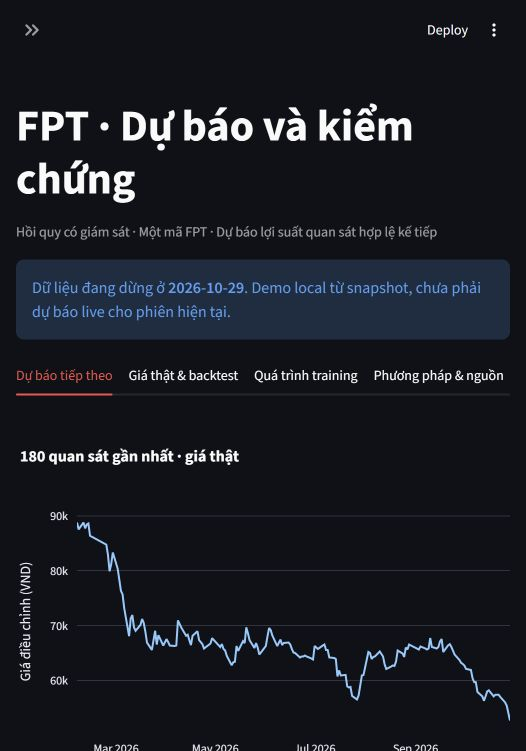
\includegraphics[width=\textwidth]{21_studio_overview_ui.png}
        \caption{Trang Tổng quan \& Phân tích kỹ thuật}
    \end{subfigure}
    \hfill
    \begin{subfigure}[b]{0.49\textwidth}
        \centering
        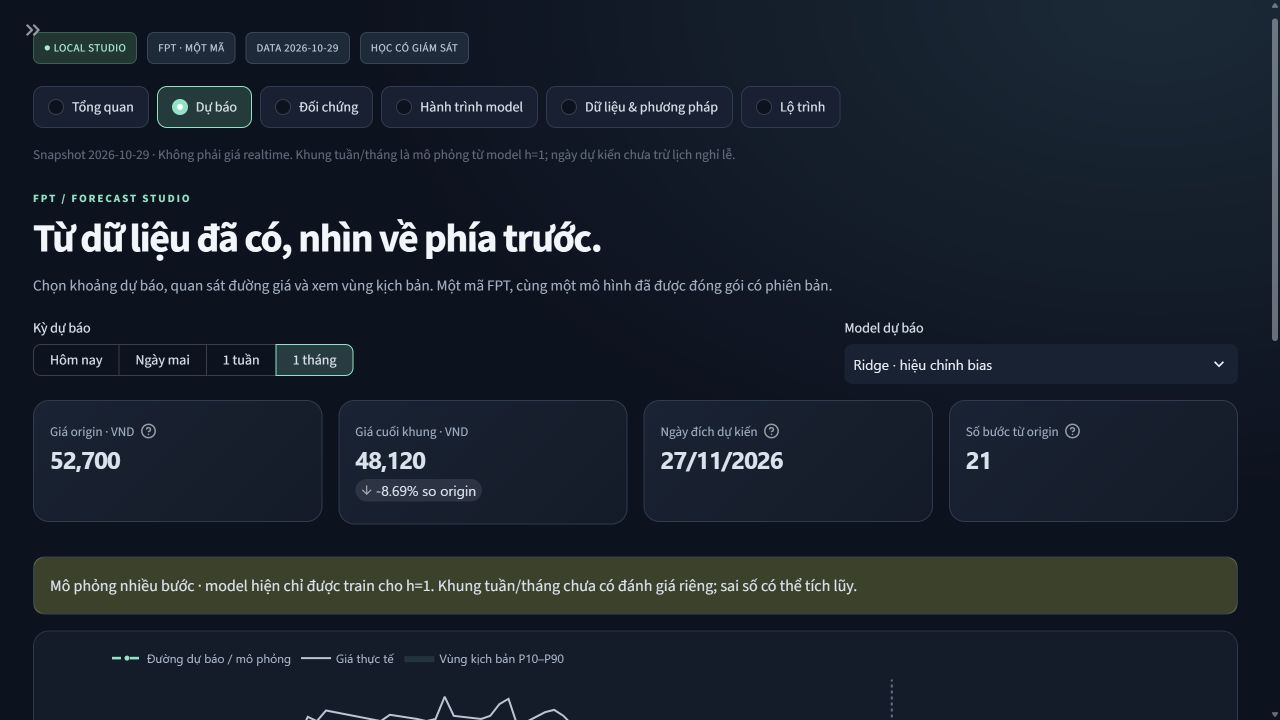
\includegraphics[width=\textwidth]{10_forecast_studio_ui.png}
        \caption{Trang Dự báo FPT Forecast Studio}
    \end{subfigure}
    \caption{Giao diện ứng dụng thực tế FPT Forecast Studio chạy kết nối trực tiếp với FastAPI.}
    \label{fig:ch5_studio_ui_pair}
\end{figure}

\begin{figure}[H]
    \centering
    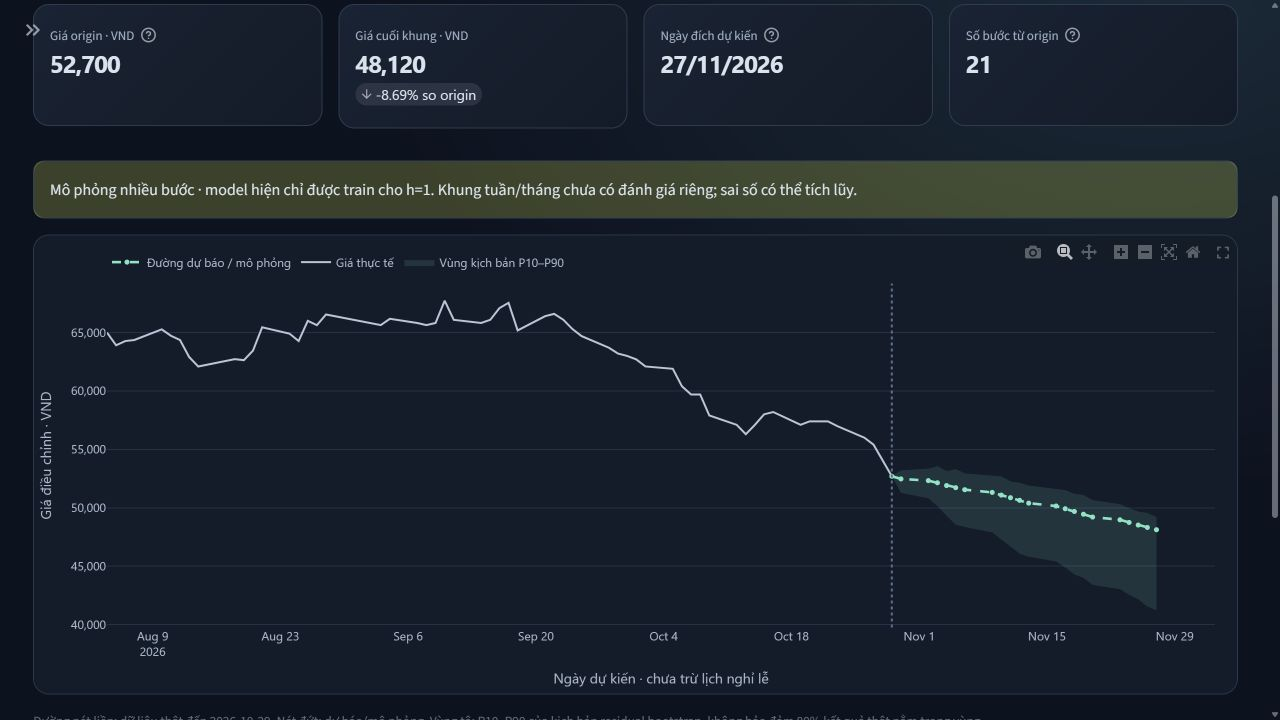
\includegraphics[width=0.90\textwidth]{18_forecast_month_ui.png}
    \caption{Minh họa kết quả mô phỏng 1 tháng kèm dải kịch bản P10--P90 trên giao diện Forecast Studio.}
    \label{fig:ch5_month_ui}
\end{figure}

\subsection{Hệ thống kiểm thử tự động toàn diện (149 Unit Tests)}
Chất lượng mã nguồn và tính toàn vẹn khoa học được bảo vệ bởi \textbf{149 bài kiểm thử tự động} phân bổ đều trên \textbf{20 tệp kiểm thử} trong thư mục \texttt{tests/}:
\begin{itemize}
    \item \textbf{Kiểm tra dữ liệu và chống rò rỉ (43 tests):} \nolinkurl{test_data_pipeline} (14), \nolinkurl{test_source_audit} (9), \nolinkurl{test_source_comparison} (8), \nolinkurl{test_inference_contract} (4), \nolinkurl{test_snapshot} (3), \nolinkurl{test_market_analysis} (5) — khóa chặt điều kiện train-only scaling, boundary purging và từ chối giá tương lai.
    \item \textbf{Kiểm tra thực nghiệm mô hình và hồi cứu (59 tests):} \nolinkurl{test_modeling} (8), \nolinkurl{test_robustness} (6), \nolinkurl{test_window_comparison} (3), \nolinkurl{test_ridge_refinement} (6), \nolinkurl{test_evaluation_2026} (5), \nolinkurl{test_recency_bias} (9), \nolinkurl{test_direction_selective} (11), \nolinkurl{test_candle_ablation} (7), \nolinkurl{test_final_window_comparison} (4) — xác minh độ khớp tính toán và hash SHA-256.
    \item \textbf{Kiểm tra suy luận đệ quy, API và toàn vẹn tài liệu (47 tests):} \nolinkurl{test_forecast_path} (20), \nolinkurl{test_horizon_calibration} (7), \nolinkurl{test_local_demo} (9), \texttt{test\_api} (7), \nolinkurl{test_research_notes} (4) — bảo đảm bias chỉ cộng bước 1, centering không ép tổng nhiễu về 0, HTTP API trả đúng offline và mã băm nhật ký lịch sử không bị chỉnh sửa.
\end{itemize}

\section{Giới hạn hiện tại của đồ án}
Bên cạnh các kết quả đạt được, đồ án vẫn còn bốn giới hạn kỹ thuật và thực nghiệm cần lưu ý:
\begin{enumerate}
    \item \textbf{Biên lợi thế độ lớn còn mỏng:} Dù \texttt{Ridge+bias60} cải thiện Balanced Accuracy ($56,62\%$--$57,95\%$) và giảm MAE giá trên tập kiểm định 2026, mức cải thiện MSE Skill trên lợi suất so với \nolinkurl{Zero-Return} ở $h=1$ chỉ đạt khoảng $+0,041\%$ với khoảng tin cậy 95\% vẫn chứa giá trị 0. Do đó, mô hình chưa đủ cơ sở để khẳng định lợi thế dự báo ổn định dài hạn trên thị trường thực.
    \item \textbf{Bản chất mô phỏng của dự báo tuần và tháng:} Mô hình chỉ được huấn luyện tối ưu cho kỳ hạn một phiên ($h=1$). Trong backtest 121 ngày gốc ở $h=5$ và $h=22$, dự báo điểm đệ quy vẫn có RMSE cao hơn chuẩn \nolinkurl{Zero-Return}. Do đó, đường tuần/tháng trên ứng dụng chỉ mang tính chất kịch bản tham khảo đi kèm dải bất định P10--P90.
    \item \textbf{Chưa tích hợp lịch nghỉ lễ đặc thù của sàn HOSE:} Hệ thống nội suy ngày giao dịch kế tiếp hiện loại trừ thứ Bảy và Chủ Nhật nhưng chưa tự động loại bỏ các dịp nghỉ lễ như Tết Nguyên Đán, 30/04 hay 02/09.
    \item \textbf{Dữ liệu điều chỉnh hồi tố và vùng P10--P90:} Giá điều chỉnh cổ tức của Vietcap có thể cập nhật lại trong lịch sử khi doanh nghiệp chia tách mới; đồng thời vùng P10--P90 dựa trên Bootstrap thực nghiệm chưa bảo đảm độ phủ $80\%$ tuyệt đối trong các giai đoạn biến động cực đoan.
\end{enumerate}

\section{Hướng phát triển tương lai}
Từ hệ thống hiện có, nhóm đề xuất bốn hướng phát triển tiếp theo:
\begin{enumerate}
    \item \textbf{Thu thập bằng chứng ngoài mẫu thực tế qua Forward Shadow Ledger:} Vận hành công cụ \nolinkurl{src/models/forward_ledger.py} để chốt dự báo trước giờ mở cửa mỗi phiên kèm chuỗi hash chống sửa ngược quá khứ, tích lũy tối thiểu 60--120 phiên quan sát tương lai hoàn toàn mới trước khi xem xét thay đổi phiên bản mô hình.
    \item \textbf{Huấn luyện mô hình dự báo trực tiếp đa kỳ hạn (\textit{Direct Multi-Horizon Forecasting}):} Thiết kế các mô hình độc lập dự đoán trực tiếp lợi suất tích lũy 5 phiên ($y_t^{(5)} = \ln(C_{t+5}/C_t)$) và 21 phiên có cơ chế loại bỏ nhãn chồng lấp (\textit{Purged Cross-Validation}), thay thế dần cơ chế lặp đệ quy từ mô hình $h=1$.
    \item \textbf{Tích hợp biến ngoại sinh và nhận diện trạng thái thị trường:} Bổ sung lợi suất chỉ số thị trường chung (VN-Index), chỉ số biến động ngành công nghệ và mô hình Markov ẩn (HMM) phân tách trạng thái biến động thấp/cao vào tập đặc trưng đầu vào một cách nhân quả.
    \item \textbf{Tự động hóa lịch sàn HOSE và triển khai đám mây có giám sát:} Tích hợp bộ lịch giao dịch HOSE chính thức, thiết lập cảnh báo trượt dữ liệu (data drift) và đóng gói Docker để triển khai hệ thống thành dịch vụ web trực tuyến.
\end{enumerate}

% ==========================================
% TÀI LIỆU THAM KHẢO (CHUẨN IEEE)
% ==========================================
\clearpage
\phantomsection
\addcontentsline{toc}{chapter}{Tài liệu tham khảo}
\begin{thebibliography}{99}

\bibitem{hoerl1970ridge}
A.~E. Hoerl and R.~W. Kennard, ``Ridge regression: Biased estimation for nonorthogonal problems,'' \textit{Technometrics}, vol.~12, no.~1, pp.~55--67, 1970.

\bibitem{hochreiter1997lstm}
S.~Hochreiter and J.~Schmidhuber, ``Long short-term memory,'' \textit{Neural Computation}, vol.~9, no.~8, pp.~1735--1780, 1997.

\bibitem{huber1964robust}
P.~J. Huber, ``Robust estimation of a location parameter,'' \textit{The Annals of Mathematical Statistics}, vol.~35, no.~1, pp.~73--101, 1964.

\bibitem{chen2016xgboost}
T.~Chen and C.~Guestrin, ``XGBoost: A scalable tree boosting system,'' in \textit{Proc. 22nd ACM SIGKDD Int. Conf. Knowledge Discovery and Data Mining (KDD)}, San Francisco, CA, USA, 2016, pp.~785--794.

\bibitem{platt1999probabilistic}
J.~Platt, ``Probabilistic outputs for support vector machines and comparisons to regularized likelihood methods,'' in \textit{Advances in Large Margin Classifiers}, MIT Press, 1999, pp.~61--74.

\bibitem{politis1992circular}
D.~N. Politis and J.~P. Romano, ``A circular block-resampling procedure for stationary data,'' in \textit{Exploring the Limits of Bootstrap}, R.~LePage and L.~Billard, Eds., Wiley, 1992, pp.~263--270.

\bibitem{kreiss2012bootstrap}
J.-P. Kreiss and S.~N. Lahiri, ``Bootstrap methods for time series,'' in \textit{Handbook of Statistics: Time Series Analysis}, vol.~30, Elsevier, 2012, pp.~3--26.

\bibitem{gneiting2007scoring}
T.~Gneiting and A.~E. Raftery, ``Strictly proper scoring rules, prediction, and estimation,'' \textit{Journal of the American Statistical Association}, vol.~102, no.~477, pp.~359--378, 2007.

\bibitem{lei2018conformal}
J.~Lei, M.~G'Sell, A.~Rinaldo, R.~J. Tibshirani, and L.~Wasserman, ``Distribution-free predictive inference for regression,'' \textit{Journal of the American Statistical Association}, vol.~113, no.~523, pp.~1094--1111, 2018.

\bibitem{hyndman2021fpp3}
R.~J. Hyndman and G.~Athanasopoulos, \textit{Forecasting: Principles and Practice}, 3rd~ed. Melbourne, Australia: OTexts, 2021. [Online]. Available: \url{https://otexts.com/fpp3/tscv.html}

\bibitem{lopez2018afml}
M.~López de Prado, \textit{Advances in Financial Machine Learning}. Hoboken, NJ, USA: John Wiley \& Sons, 2018.

\bibitem{pedregosa2011sklearn}
F.~Pedregosa \textit{et al.}, ``Scikit-learn: Machine learning in Python,'' \textit{Journal of Machine Learning Research}, vol.~12, pp.~2825--2830, 2011.

\end{thebibliography}

\end{document}
